\documentclass{beamer}

% This file is a solution template for:

% Copyright 2004 by Till Tantau <tantau@users.sourceforge.net>.
%
% In principle, this file can be redistributed and/or modified under
% the terms of the GNU Public License, version 2.
%
% However, this file is supposed to be a template to be modified
% for your own needs. For this reason, if you use this file as a
% template and not specifically distribute it as part of a another
% package/program, I grant the extra permission to freely copy and
% modify this file as you see fit and even to delete this copyright
% notice. 

%MATH
\newcommand{\vectornorm}[1]{\left|\left|#1\right|\right|}
\newcommand{\spectralnorm}[1]{\left|\left|#1\right|\right|_{2}}


%\mode<presentation>
%{
	%\usetheme{Oxygen}
%}

\usecolortheme[color=white]{robolabo}

\usepackage[spanish]{babel}
% or whatever
\usepackage{amssymb}
\usepackage{amsmath}

\usepackage[utf8x, utf8]{inputenc}
% or whatever

\usepackage{times}
\usepackage[T1]{fontenc}
\usepackage{color}
%\usepackage{natbib}
\usepackage[official]{eurosym}
\newcommand{\spacing}{1.5}

\usepackage{multimedia}
\usepackage{hyperref}
% Or whatever. Note that the encoding and the font should match. If T1
% does not look nice, try deleting the line with the fontenc.
\usepackage{thumbpdf}
\usepackage{wasysym}
\usepackage{ucs}
\usepackage{pgf,pgfarrows,pgfnodes,pgfautomata,pgfheaps,pgfshade}
\usepackage{verbatim}
\usepackage{colortbl}
\usepackage{multirow}
%\usepackage{xfrac}
\usepackage{ragged2e}

%\usepackage{graphicx}
\usepackage{animate}
\usepackage{tikz}
\usetikzlibrary{	
	calc
}
\newcommand*{\ClipSep}{0.4cm}%

%For the pictures
\usepackage{epic}\setlength{\unitlength}{1cm}
\usepackage{eepic}\setlength{\unitlength}{1cm}
\usepackage{longtable}
\usepackage{array}
\usepackage{units}
\usepackage{lipsum}
\usepackage{etoolbox}

\newtoggle{video}
\togglefalse{video}

\setbeamertemplate{navigation symbols}{}%remove navigation symbols

\newcommand{\avgcc}[1]{\textit{avg}\left(\rho^i[l^i#1]\right)}
\newcommand{\varcc}[1]{\textit{var}\left(\rho^i[l^i#1]\right)}

%\title[ Swarm Grid ]
%{\Large A swarm intelligence approach based on coupled oscillators: \\ an application in demand side management with photovoltaic distributed generation}


%\author[M. Castillo Cagigal]{
  %Manuel Castillo Cagigal%\inst{1}
%}

%\institute{
%  $^{1}$ETSIT, Universidad Polit\'ecnica de Madrid, Madrid, Spain   
%}



%\date{December 5, 2014}
%\date{}

%\author[Manuel Castillo-Cagigal] % (optional, use only with lots of authors)
%{Manuel Castillo Cagigal}

% - Use the \inst{?} command only if the authors have different
%   affiliation.


%\institute[IES-UPM] % (optional, but mostly needed)
%{\textbf{Máster de Domótica y Hogar Digital} \\ \vspace{0.5cm} IES-UPM}


\title{De Sociedades de Insectos a\\ \vspace{0.2cm}Comunidades Energéticas: \\\vspace{0.4cm}\large{Liberando la Gestión\\ \vspace{0.2cm}Distribuida de la Demanda}}
%\subtitle{R\&D in GEDIRCI}
%\author[\'{A}lvaro Guti\'{e}rrez]{\'{A}lvaro Guti\'{e}rrez}
\author[\'{A}lvaro Guti\'{e}rrez]{\hspace{0.5cm}}
\institute[]{\vspace{0.5cm}Prof. Álvaro Gutiérrez Martín\\
Laboratorio de Robótica y Control\\
Generación Distribuida Renovable y Control Inteligente\\
E.T.S. Ingenieros de Telecomunicación\\
Universidad Politécnica de Madrid\\
\hspace{0.5cm}}
\date{\Large{09/11/2026}}
\tikzset{
  invisible/.style={opacity=0},
    visible on/.style={alt=#1{}{invisible}},
    alt/.code args={<#1>#2#3}{%
      \alt<#1>{\pgfkeysalso{#2}}{\pgfkeysalso{#3}} % \pgfkeysalso doesn't change the path
    },
}

\subject{Charlas}

\AtBeginSubsection[]
{
  \frame<handout:0>
  {
    \frametitle{Contenido}
    \tableofcontents[sectionstyle=show/hide,subsectionstyle=show/shaded/hide]
  }
}

\newcommand<>{\highlighton}[1]{%
  \alt#2{\structure{#1}}{{#1}}
}

\newcommand{\icon}[1]{\pgfimage[height=1em]{#1}}

\begin{document}
\def\newblock{\hskip .11em plus .33em minus .07em}
\graphicspath{{figs/}}


\begin{frame}[plain]
  \titlepage
\end{frame}

%\begin{frame}[plain]
  %\begin{columns}
    %\begin{column}{\paperwidth}
      %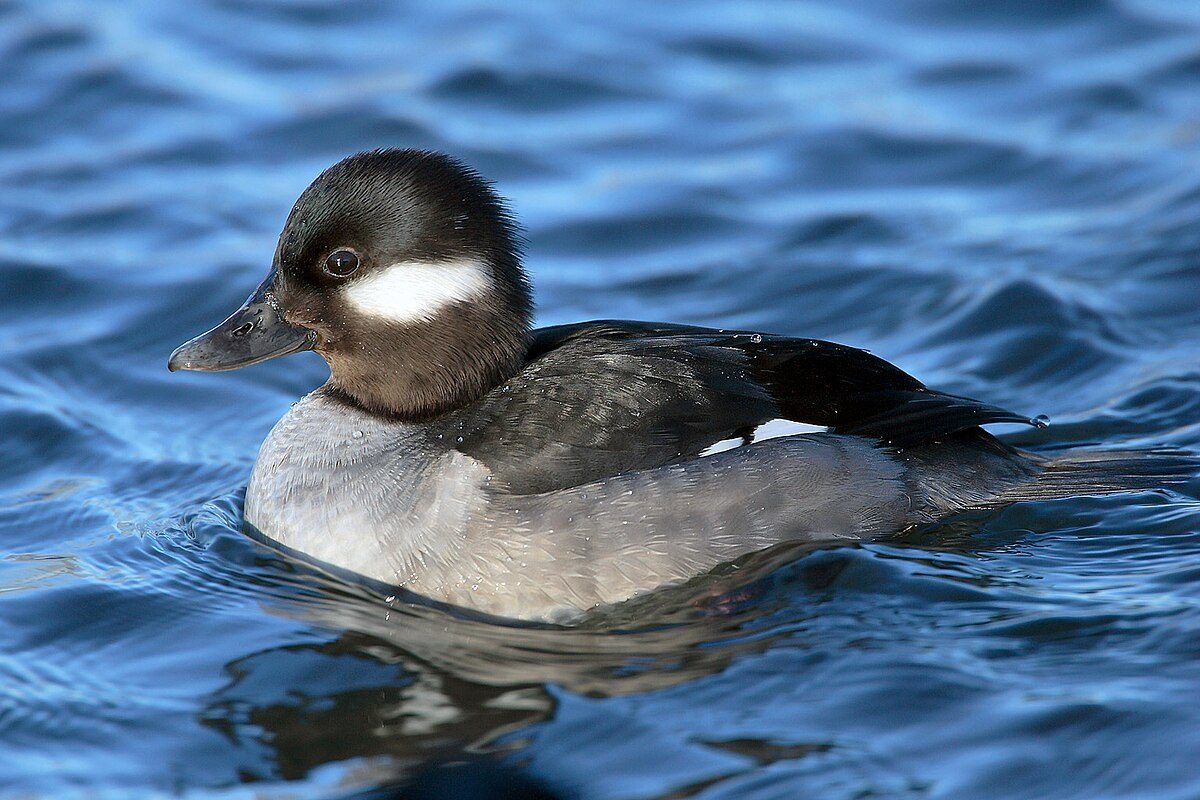
\includegraphics[height=\paperheight,width=\paperwidth]{duck}
    %\end{column}
  %\end{columns}
%\end{frame}
%+++++++++++++++++++++++++++++++++++++++++++++++++++++++++++++++++++++++++%
\section*{Introducción}

\begin{frame}
  \frametitle{\textcolor{white}{Introducción}}
	\begin{center}
    {\large{\textbf{De las Sociedades de Insectos a las Comunidades Energéticas Locales}:} \\\vspace{0.1cm}\large{Liberando la Gestión Distribuida de la Demanda}}\\
    \vspace{0.1cm}

    \begin{tikzpicture}
      \node [inner sep=0pt] at (0,0) {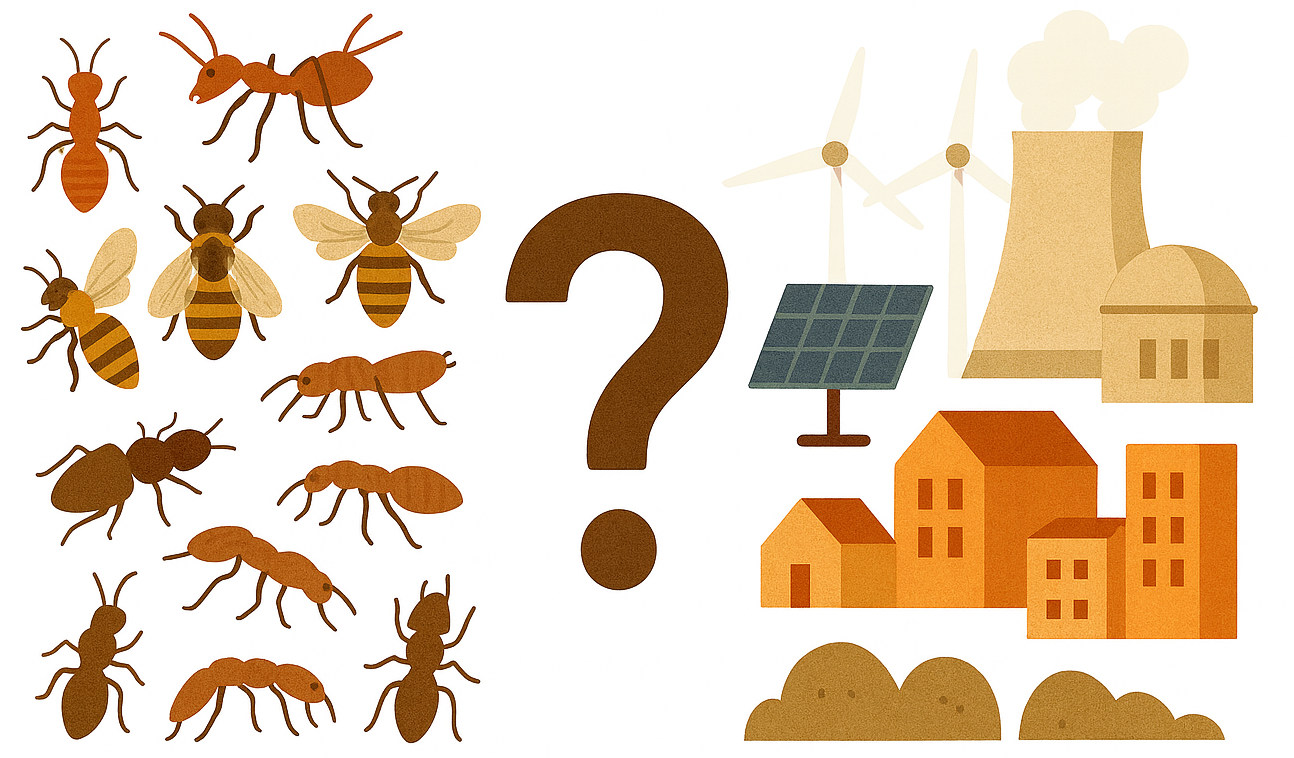
\includegraphics[width=10cm]{intro0_white}};
      \draw [white, rounded corners=\ClipSep, line width=\ClipSep] 
      (current bounding box.north west) -- 
      (current bounding box.north east) --
      (current bounding box.south east) --
      (current bounding box.south west) -- cycle
      ;
    \end{tikzpicture}
	\end{center}
\end{frame}

%%------------%

%%------------%
\begin{frame}
  \frametitle{Sistema eléctrico}
	\begin{center}
	{\bf Regla principal}\\
	La generación y el consumo deben coincidir instantáneamente\\[0.1cm]
	
\includegraphics[width=10cm]{instantaneousConcept3_white}\\
    %\begin{tikzpicture}
      %\node [inner sep=0pt] at (0,0) {
\includegraphics[width=10cm]{instantaneousConcept3_white}};
      %\draw [white, rounded corners=\ClipSep, line width=\ClipSep] 
      %(current bounding box.north west) -- 
      %(current bounding box.north east) --
      %(current bounding box.south east) --
      %(current bounding box.south west) -- cycle
      %;
    %\end{tikzpicture}
	Origen de los principales problemas...
	\end{center}
\end{frame}

%------------%
\begin{frame}
	\frametitle{Sistema eléctrico}
  \vspace{0.4cm}
	\begin{center}	
    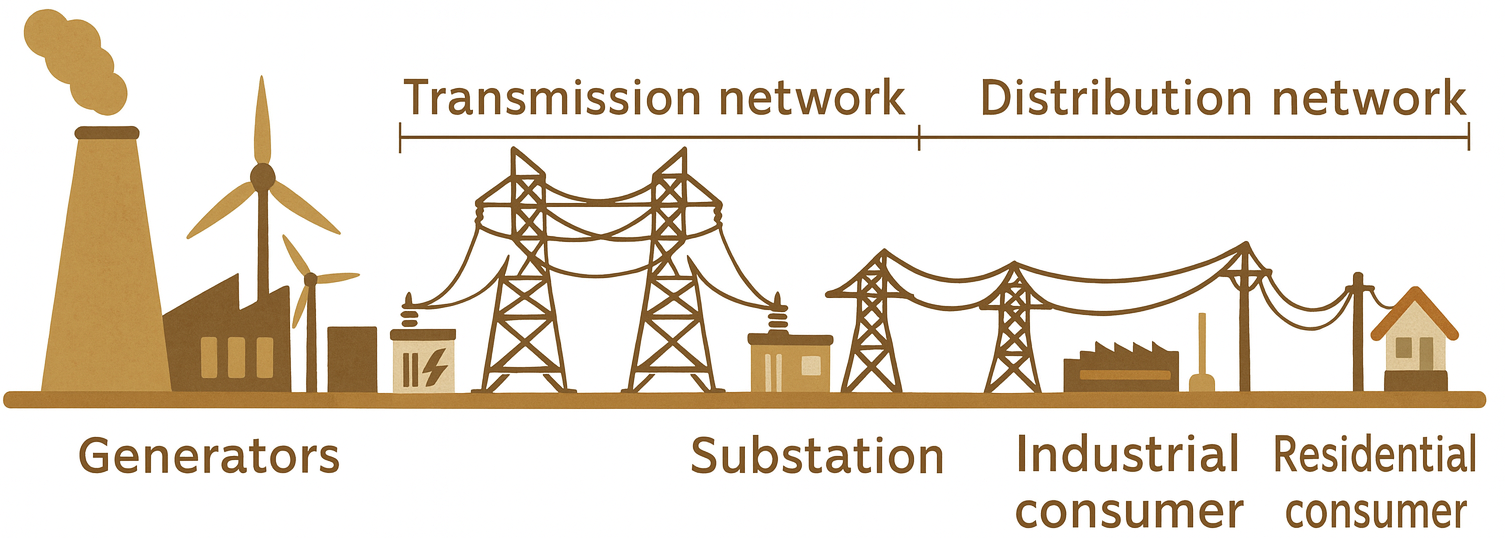
\includegraphics[width=11cm]{gridSketch2_white}
	\end{center}
	%\begin{itemize}
	  %\item{{\bf Generators}: }produce electric power from primary sources.
	  %\item{{\bf Transmission network}: }from power plants to substations.
	  %\item{{\bf Substations}: }power conditioning and safety mechanism.
	  %\item{{\bf Distribution network}: }from substations to consumers.
	  %\item{{\bf Consumption}: }transforms electric power into work.
	%\end{itemize}
\end{frame}
%------------%

\begin{frame}
  \frametitle{Sistema eléctrico}
	\begin{center}
	  \includegraphics[width=11cm]{gridGeneration_v2.eps}
    %\begin{columns}
      %\column{4cm}
        %\centering
        %\begin{itemize}
          %\item Centralized
          %\item $\downarrow$ Efficiency 
          %\item $\downarrow$ Communication 
        %\end{itemize}
      %\column{4cm}
      %\begin{itemize}
        %\item Distributed
        %\item $\uparrow$ Integration
        %\item $\uparrow$ Participation
      %\end{itemize} 
    %\end{columns} 
	\end{center}
  \pause
    \vspace{0.5cm}
    \centering{\huge{¿Cómo coordinar?}}
\end{frame}

%------------%
\begin{frame}
  \frametitle{Curva de demanda}
	\begin{center}	
    %\begin{tikzpicture}
      %\node [inner sep=0pt] at (0,0) {\includegraphics<1>[width=11cm]{demandElec1}};
      %\draw [white, rounded corners=\ClipSep, line width=\ClipSep] 
      %(current bounding box.north west) -- 
      %(current bounding box.north east) --
      %(current bounding box.south east) --
      %(current bounding box.south west) -- cycle
      %;
    %\end{tikzpicture}
	\includegraphics<1>[width=10cm]{demandaelec1}
	\includegraphics<2>[width=10cm]{demandaelec2}
	\end{center}
\end{frame}
%------------%

%------------%
\begin{frame}
  \frametitle{Curva de demanda}
	\begin{center}	
	{\bf La generación debe adaptarse al consumo}\\[1cm]
		\begin{columns}
		\column{6cm}
			\includegraphics<1>[width=6cm]{demandaelec_derivate}
			\includegraphics<2>[width=6cm]{demandaelec_peak} \\
		\column{6cm}
			Problemas:
			\begin{itemize}
			\item{{\bf Capacidad de respuesta}: }
			\begin{itemize}
				\item{Disponibilidad tecnológica}
				\item{Estrés del sistema}
			\end{itemize}
			\visible<2>{
			\item{{\bf Tamaño de la red}: }
				\begin{itemize}
					\item{Sobredimensionado de la generación}
					\item{Sobredimensionado de las líneas}
				\end{itemize}
			}
			\end{itemize}			
		\end{columns}
	\end{center}
\end{frame}

%------------%
%\begin{frame}
  %\frametitle{Demand curve}
  %\begin{center}	
	  %\input{animations/demandSmooth.code}
  %\end{center}
%\end{frame}
%------------%

\begin{frame}
  \frametitle{Gestión de la Demanda (DSM): Enfoque individual}
  \begin{columns}
    \column{5.5cm}
    \includegraphics[width=4cm]{figs/magicbox.eps}
    \column{5.5cm}
    \begin{itemize}
      \item Generación FV
      \item Consumo de las cargas
    \end{itemize}
  \end{columns}
  \vspace{0.5cm}
  \begin{center}
    \begin{tabular}{cc}
      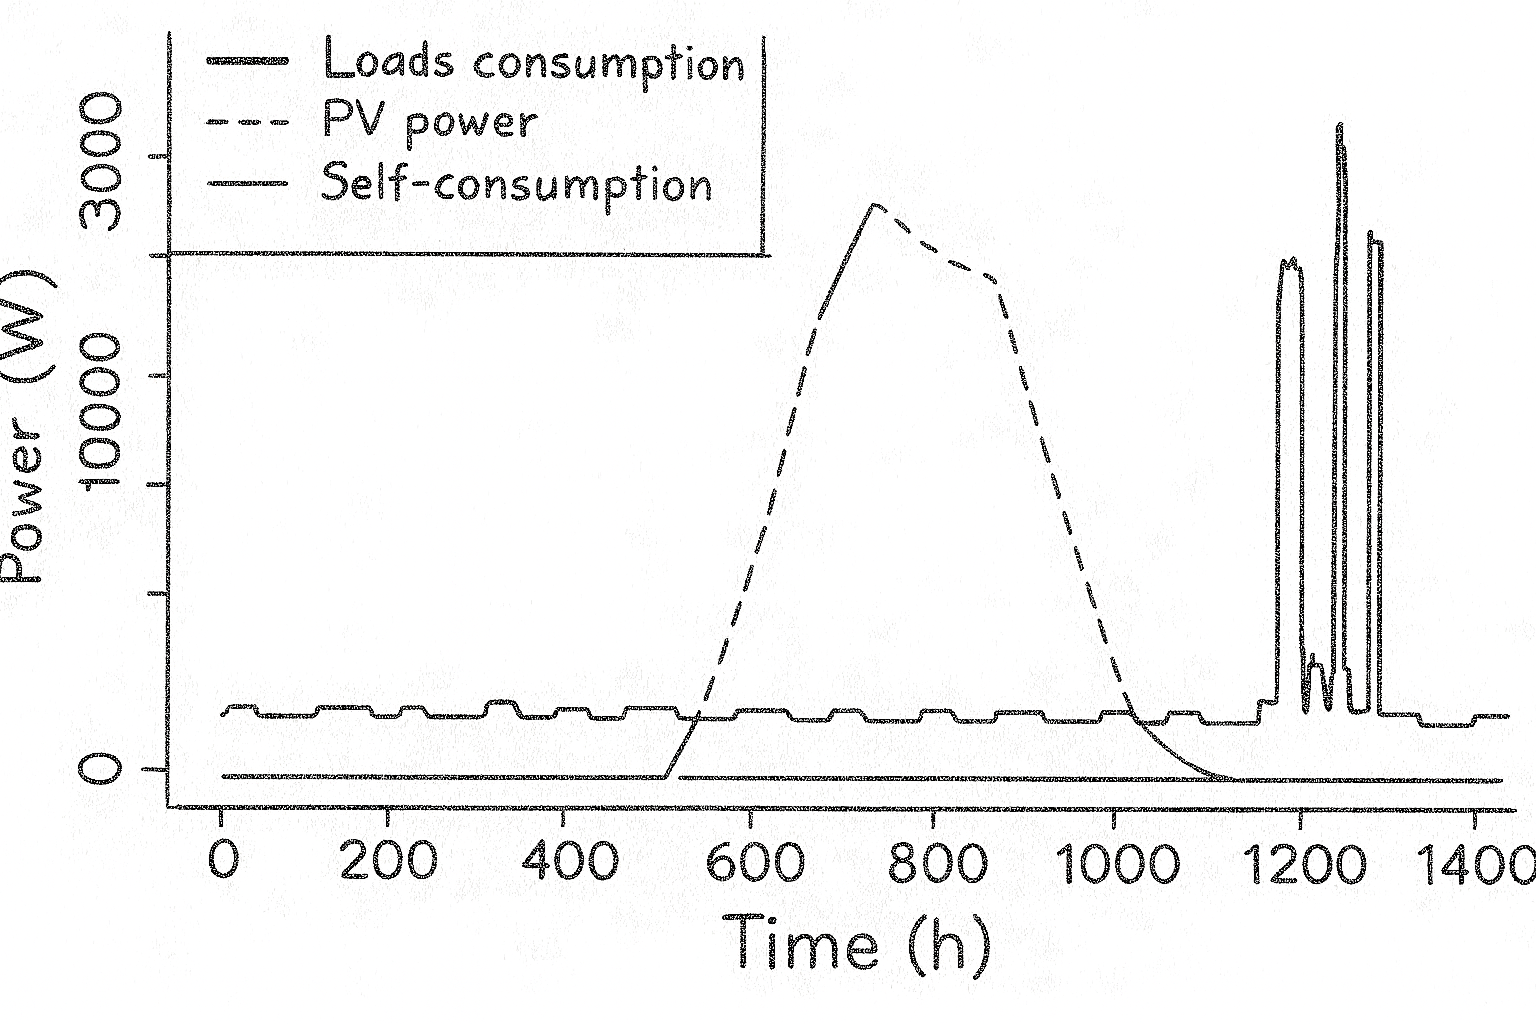
\includegraphics[width=5cm]{figs/plot_withoutADSM_scketch_white} &
      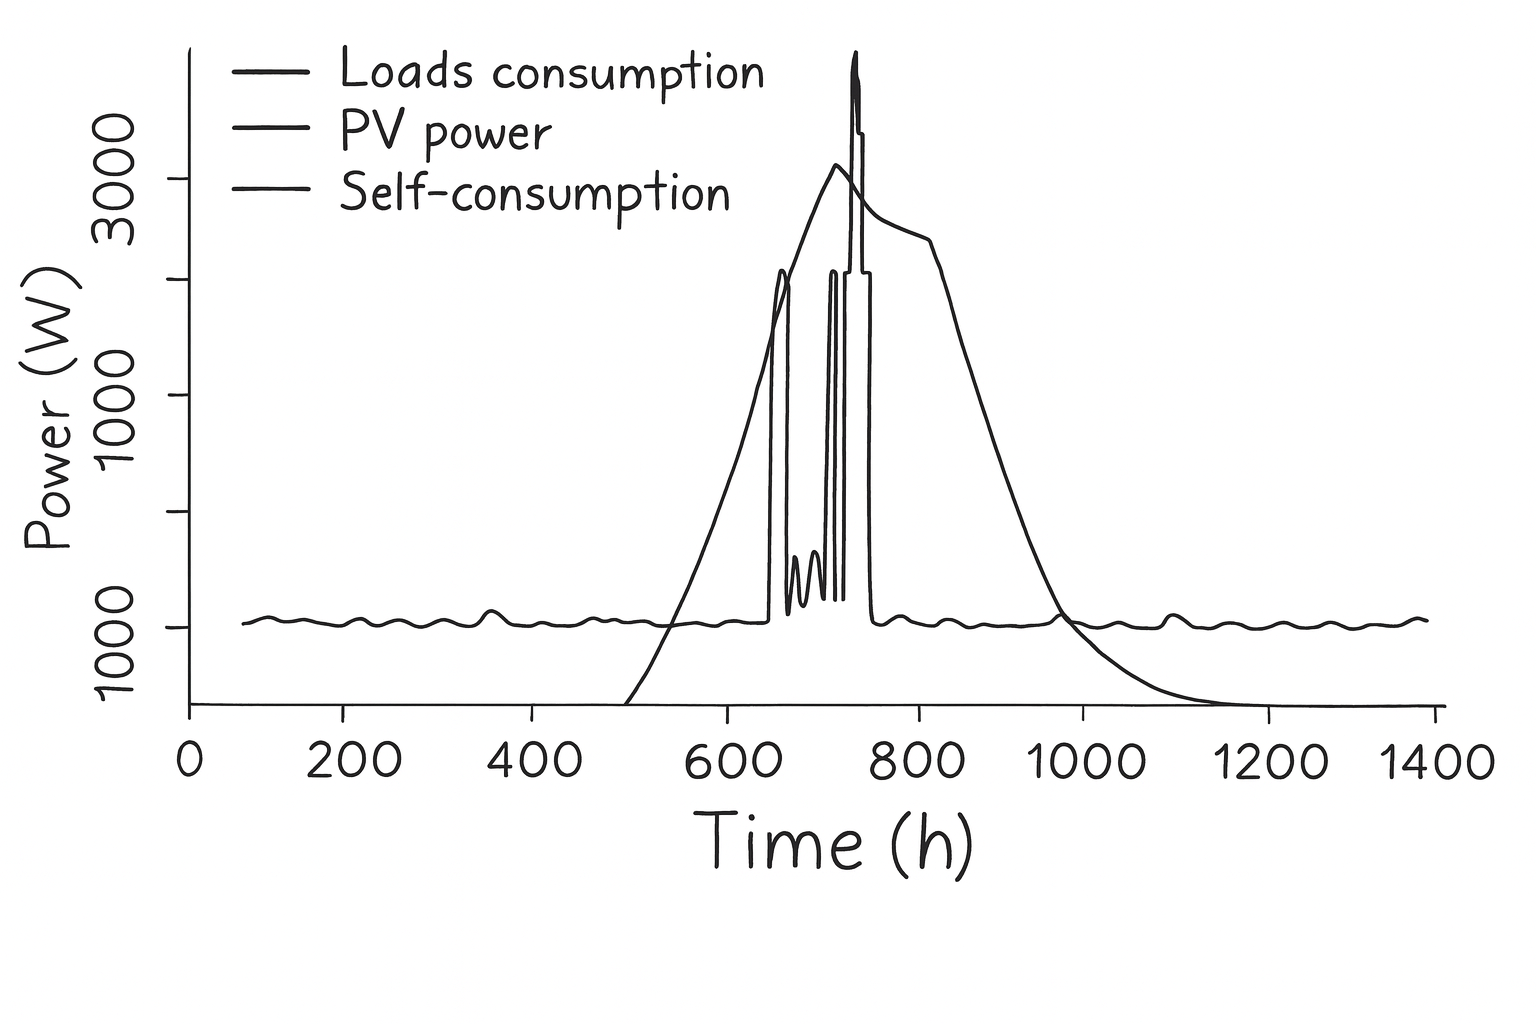
\includegraphics[width=5cm]{figs/plot_withADSM_scketch_white}\\
    \end{tabular}
  \end{center}
\end{frame}

\begin{frame}
  \frametitle{Sistema eléctrico}
	\begin{center}
	  \includegraphics[width=11cm]{figs/gridGeneration_v2.eps}
		\vspace{0.2cm}
	\end{center}
	\begin{center}
		\includegraphics<1>[width=1.5cm]{figs/question.eps}
		\includegraphics<2>[width=6cm]{figs/multihouse_v2}

    \only<3>
    {
      %\begin{center}
			{\Large \textbf{¿Cómo organizar?}} \\
        \vspace{0.2cm}
			{\Large\textbf{¿Cómo coordinar?}}
			%{\Large\textbf{How to communicate?}}
	%\end{center}
}
	\end{center}
\end{frame}

\begin{frame}
	\frametitle{Confusión actual}
  \begin{tabular}{cc}
    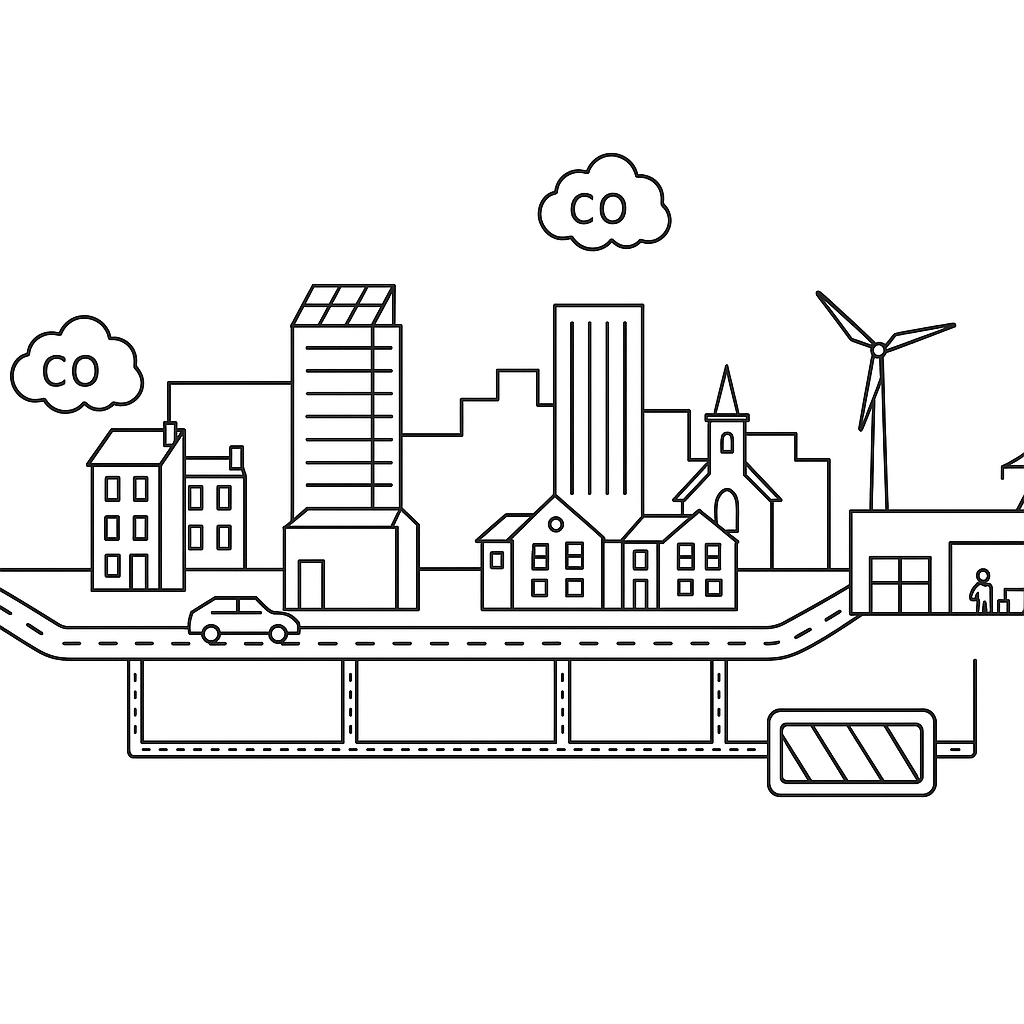
\includegraphics[width=5cm]{figs/PEDS1} &
    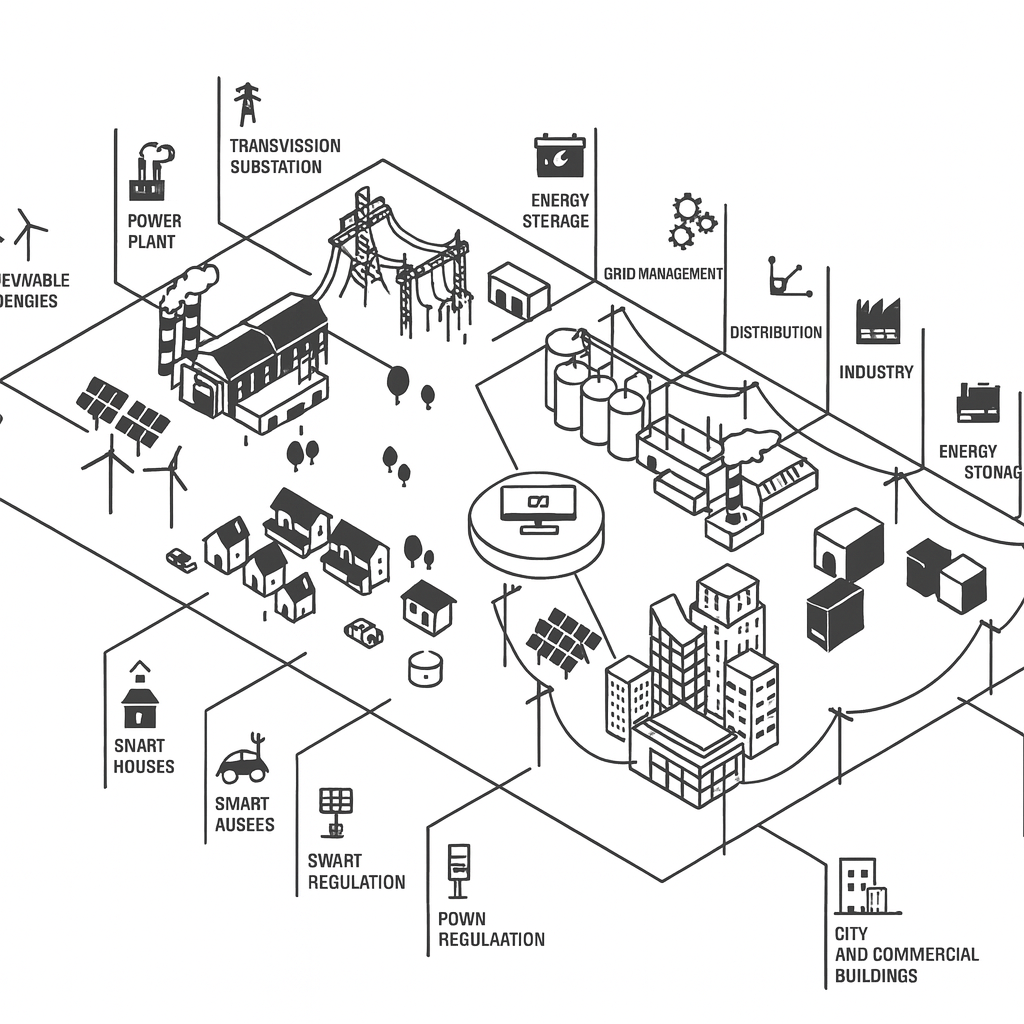
\includegraphics[width=5cm]{figs/PEDS2} \\
  \end{tabular}

  \begin{columns}
    \column{6cm}
    \begin{itemize}
      \item Autoconsumo compartido
      \item Comunidades Energéticas Locales
      \item Distritos de Energía Positiva
    \end{itemize}
    \column{4cm}
    
\includegraphics[width=3cm]{figs/PEDS3}
  \end{columns}
\end{frame}

\begin{frame}
	\frametitle{Legislación de los países}
  \footnotesize{
    \begin{itemize}
      %\item \textbf{Spain}: 2 km (Real Decreto-ley 20/2022).
      %\item \textbf{France}: 20 km in rural. 10 km peri-urban (Arr\^{e}te 19 Sept 2023)
      %\item \textbf{Portugal}: Depends on substation (Decreto-Lei 15/2022).
      %\item \textbf{Italy}: Depends on substation (REC/CEC 8/2022).
      %\item \textbf{Germany}: Adjacent geographical area  (EnWG Sec. 3, N24a)
      %\item \textbf{Netherlands}: no central km-cap; focus on net-metering transition.
      %\item \textbf{Belgium}: Regional approaches; no single all-Belgium km-cap.
      %\item \textbf{Sweden}: Collective self-consumption allowed. No simple km cap.
      %\item \textbf{Denmark}: Energy community laws (no uniform km distance).
      %\item \textbf{Poland}: Self-consumption \& energy cooperatives allowed. 
      %\item \textbf{Austria, Greece, Czechia, Romania} (and someothers): Rules based on same substation, LV/MV feeder, administrative boundary.
      \item \textbf{España} y \textbf{Francia}: normas basadas en distancia
      \item \textbf{Portugal} e \textbf{Italia}: normas basadas en la subestación
      \item \textbf{Alemania} y \textbf{Países Bajos}: normas basadas en criterios geográficos
      \item \textbf{Bélgica}: diferenciación regional
      \item \textbf{Suecia}, \textbf{Dinamarca} y \textbf{Polonia}: marcos permisivos/abiertos
      \item \textbf{Resto}: normas basadas en la misma subestación, alimentador BT/MT, límite administrativo,...
    \end{itemize}}
  \begin{center}
    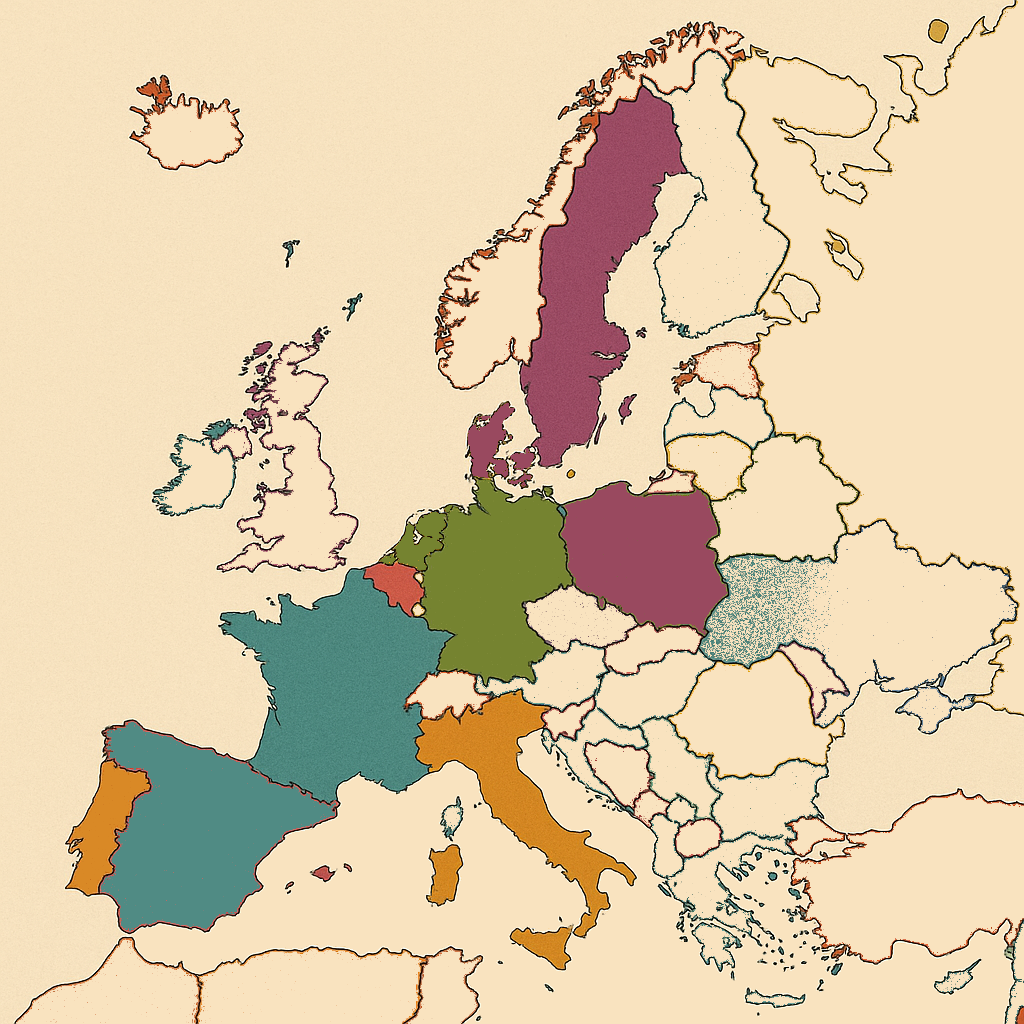
\includegraphics[width=4cm]{figs/europeMap}
  \end{center}
\end{frame}

\begin{frame}
	\frametitle{Legislación de los países}
  \vspace{0.5cm}
  %\begin{center}
    %\begin{tabular}{ccc}
      %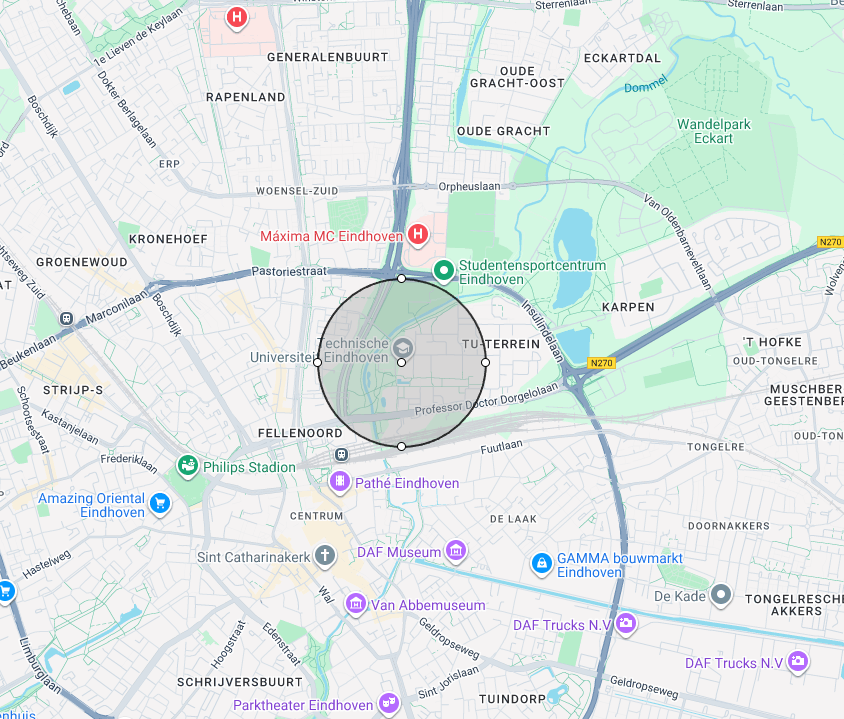
\includegraphics[width=4.5cm]{figs/eindhoven0}&
      %
\includegraphics[width=1.5cm]{figs/arrowRight}&
      %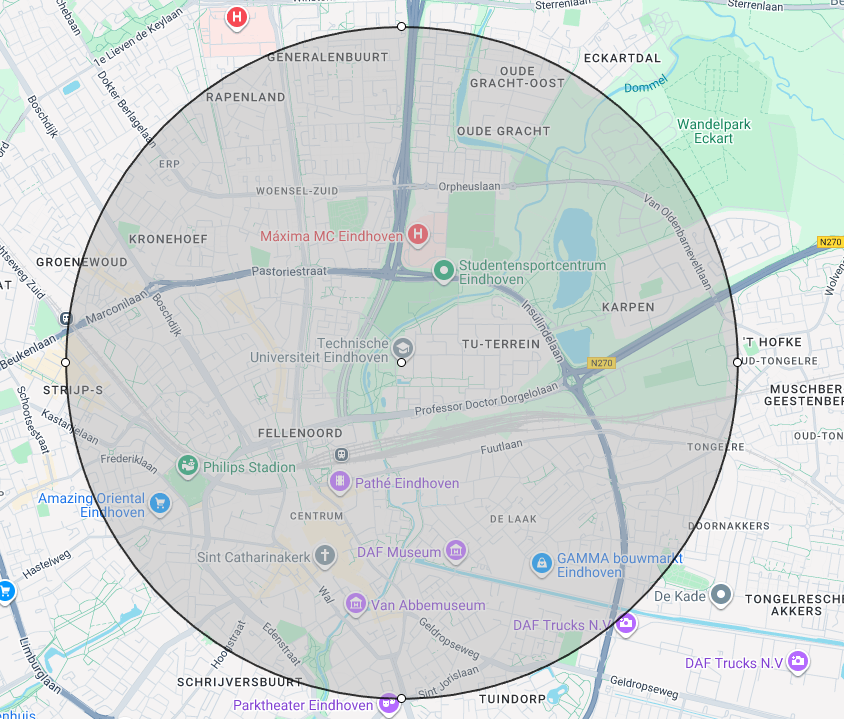
\includegraphics[width=4.5cm]{figs/eindhoven1}\\
      %\textbf{Before 2022} && \textbf{After 2022}\\
      %Very rigid system & & Very rigid system\\
      %500m from generator & & 2km from generator\\ 
    %\end{tabular}
    \hspace{-1cm}
    \begin{tabular}{>{\centering\arraybackslash}m{4.5cm} c >{\centering\arraybackslash}m{4.5cm}}
      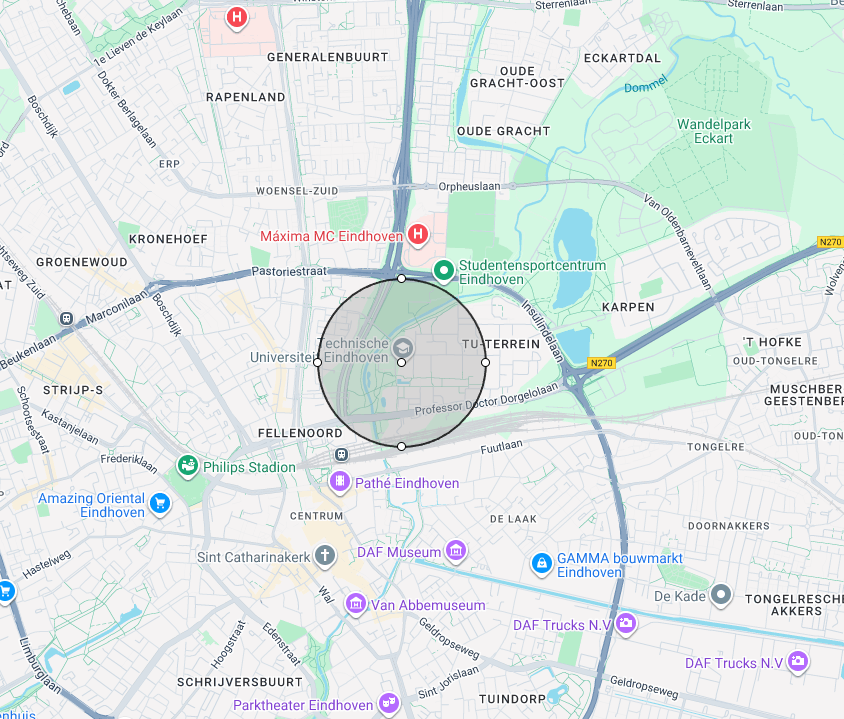
\includegraphics[width=4.5cm]{figs/eindhoven0} &
      
\includegraphics[width=1.5cm]{figs/arrowRight} &
      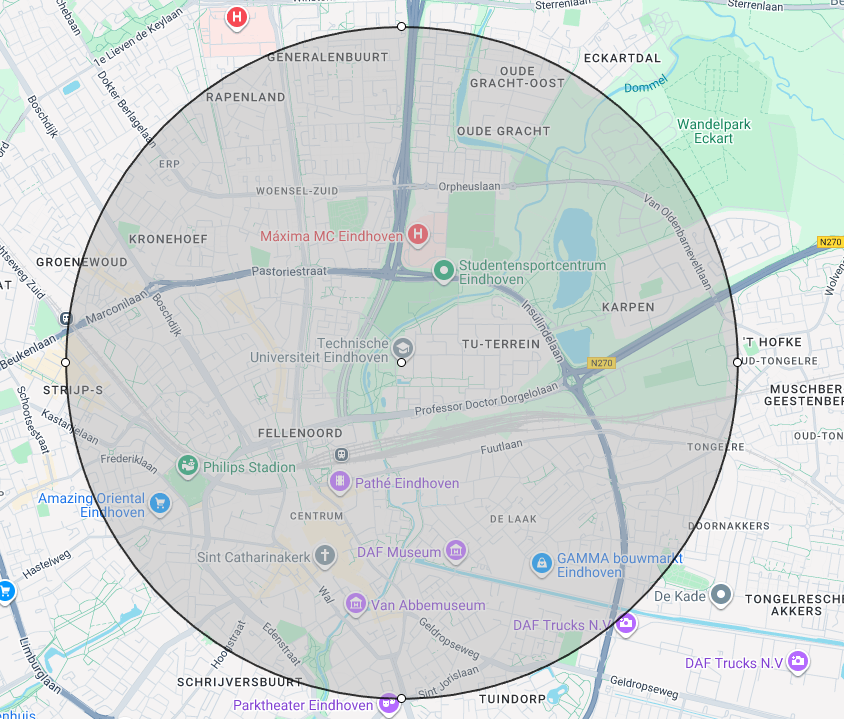
\includegraphics[width=4.5cm]{figs/eindhoven1} \\[0.3em]
      \textbf{Antes de 2022} && \textbf{Después de 2022}\\
      Sistema muy rígido & & Sistema muy rígido\\
      500m desde el generador & & 2km desde el generador\\
    \end{tabular}
  %\end{center}
\end{frame}

\begin{frame}
	\frametitle{Legislación de los países}
  \begin{center}
    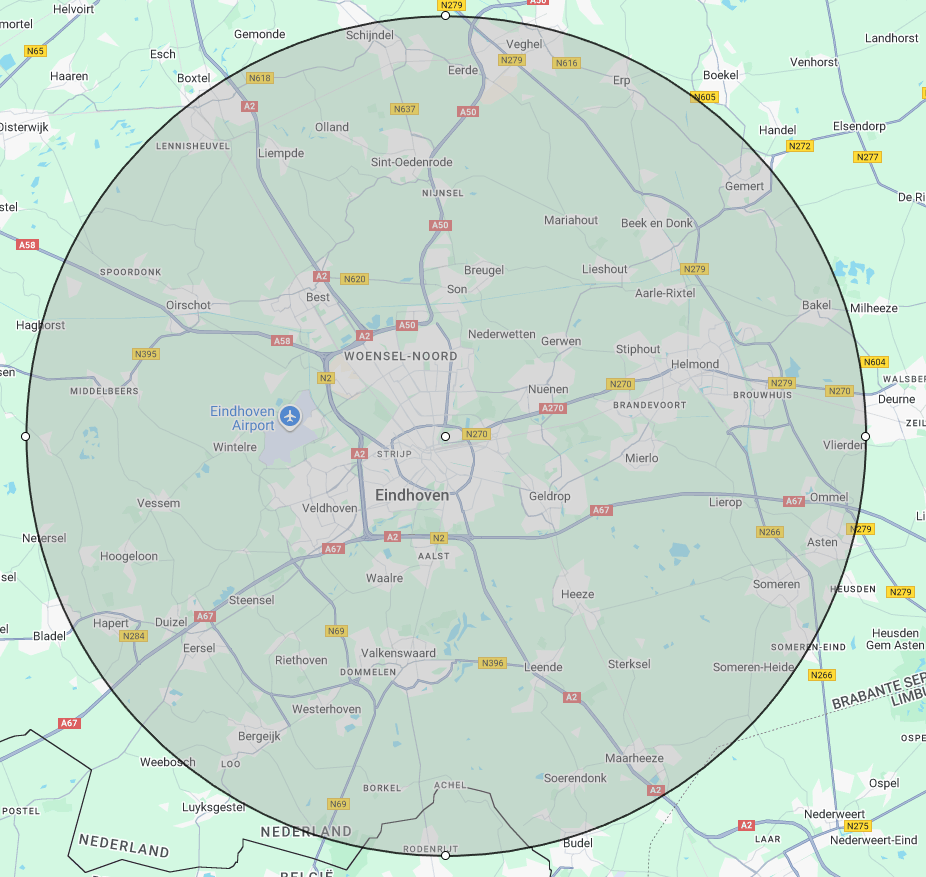
\includegraphics[width=5.5cm]{figs/eindhoven2}\\

    \textbf{Francia - 10/10/2023}\\
    \textbf{20km}\\
  \end{center}
\end{frame}

\begin{frame}
	\frametitle{Legislación de los países}
  \vspace{0.5cm}
  %\begin{center}
    %\begin{tabular}{ccc}
      %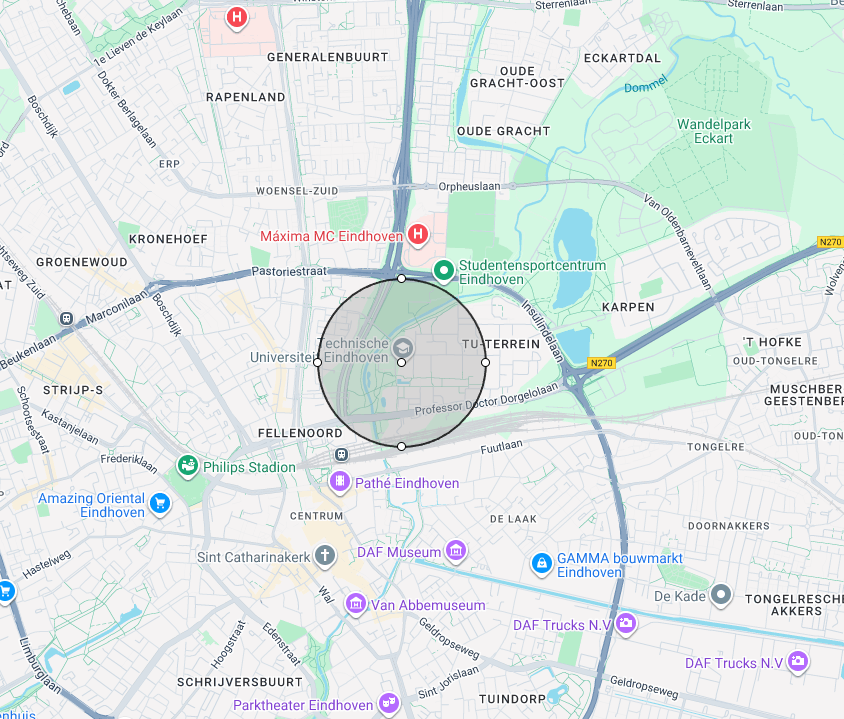
\includegraphics[width=4.5cm]{figs/eindhoven0}&
      %
\includegraphics[width=1.5cm]{figs/arrowRight}&
      %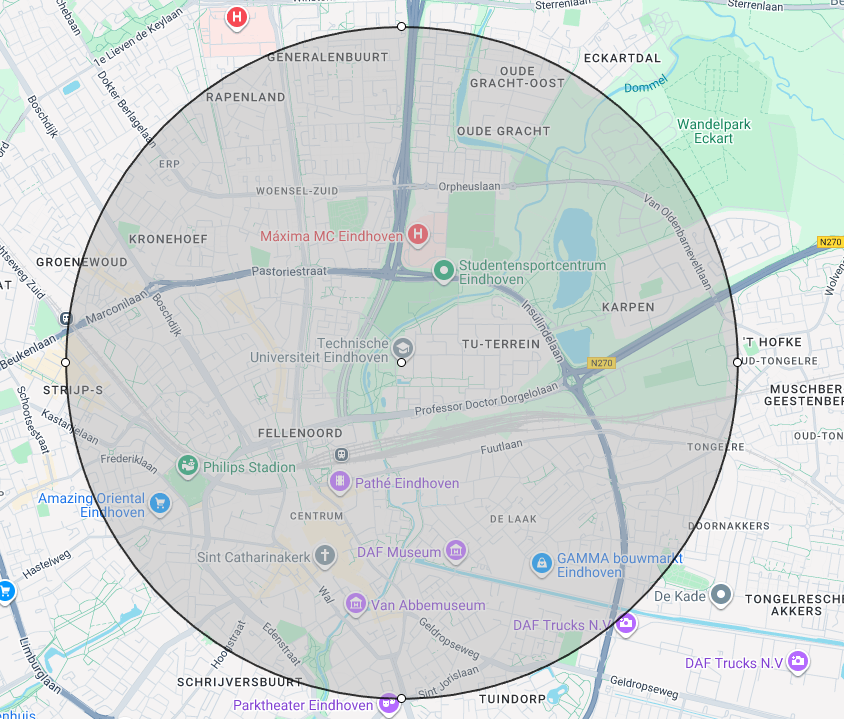
\includegraphics[width=4.5cm]{figs/eindhoven1}\\
      %\textbf{Before 2022} && \textbf{After 2022}\\
      %Very rigid system & & Very rigid system\\
      %500m from generator & & 2km from generator\\ 
    %\end{tabular}
    \hspace{-1cm}
    \begin{tabular}{>{\centering\arraybackslash}m{4.5cm} c >{\centering\arraybackslash}m{4.5cm}}
      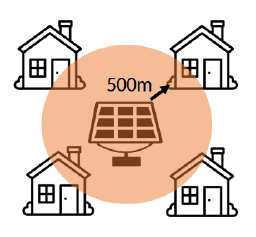
\includegraphics[width=3.5cm]{figs/legislation1} &
      
\includegraphics[width=1.5cm]{figs/arrowRight} &
      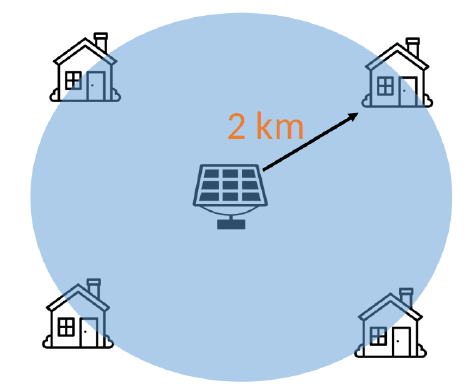
\includegraphics[width=4.5cm]{figs/legislation2} \\[0.3em]
      %\textbf{Before 2022} && \textbf{After 2022}\\
      Sistema muy rígido & & Burocrático\\
      500m/2km/20km & & Estático\\
    \end{tabular}
  %\end{center}
\end{frame}

\begin{frame}
  \frametitle{Futuro deseado}
  \begin{center}
    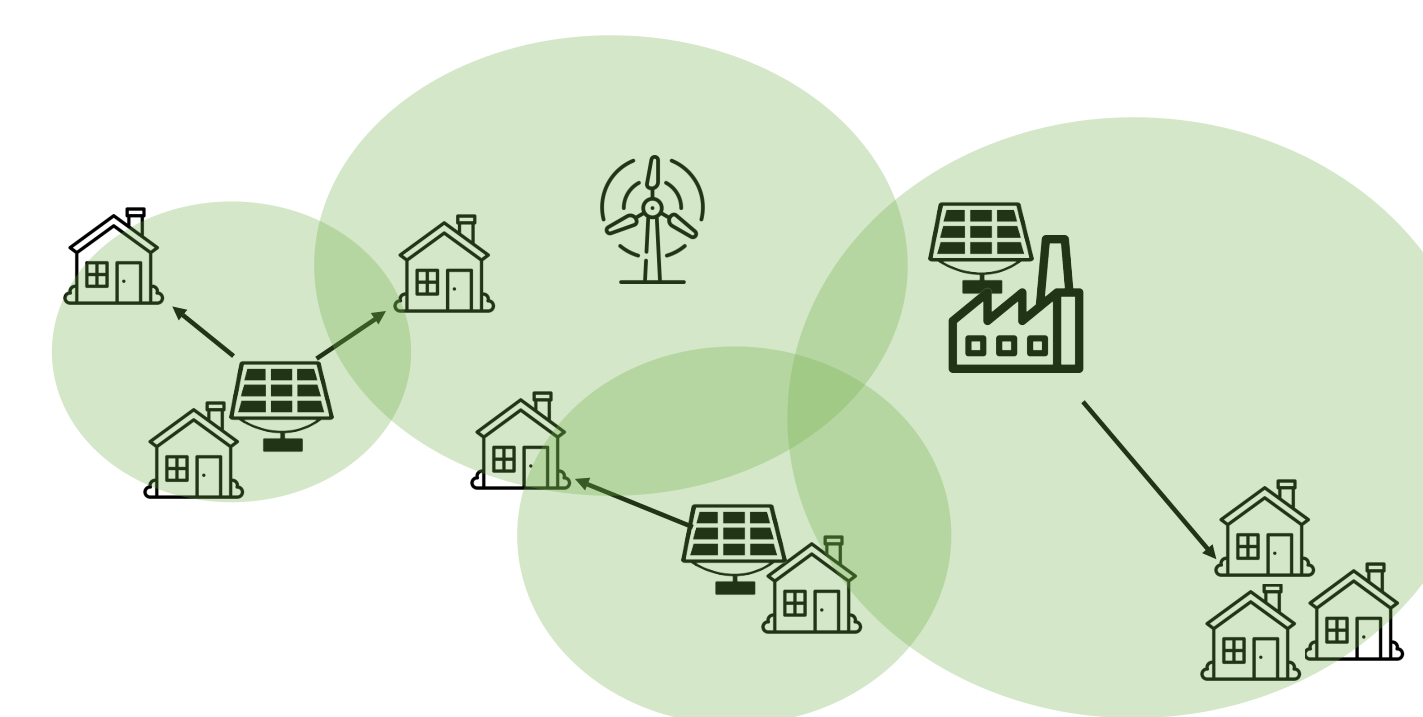
\includegraphics[width=11cm]{figs/huawei5}
  \end{center}
\end{frame}

\begin{frame}
  \frametitle{Futuro deseado}
  \begin{center}
    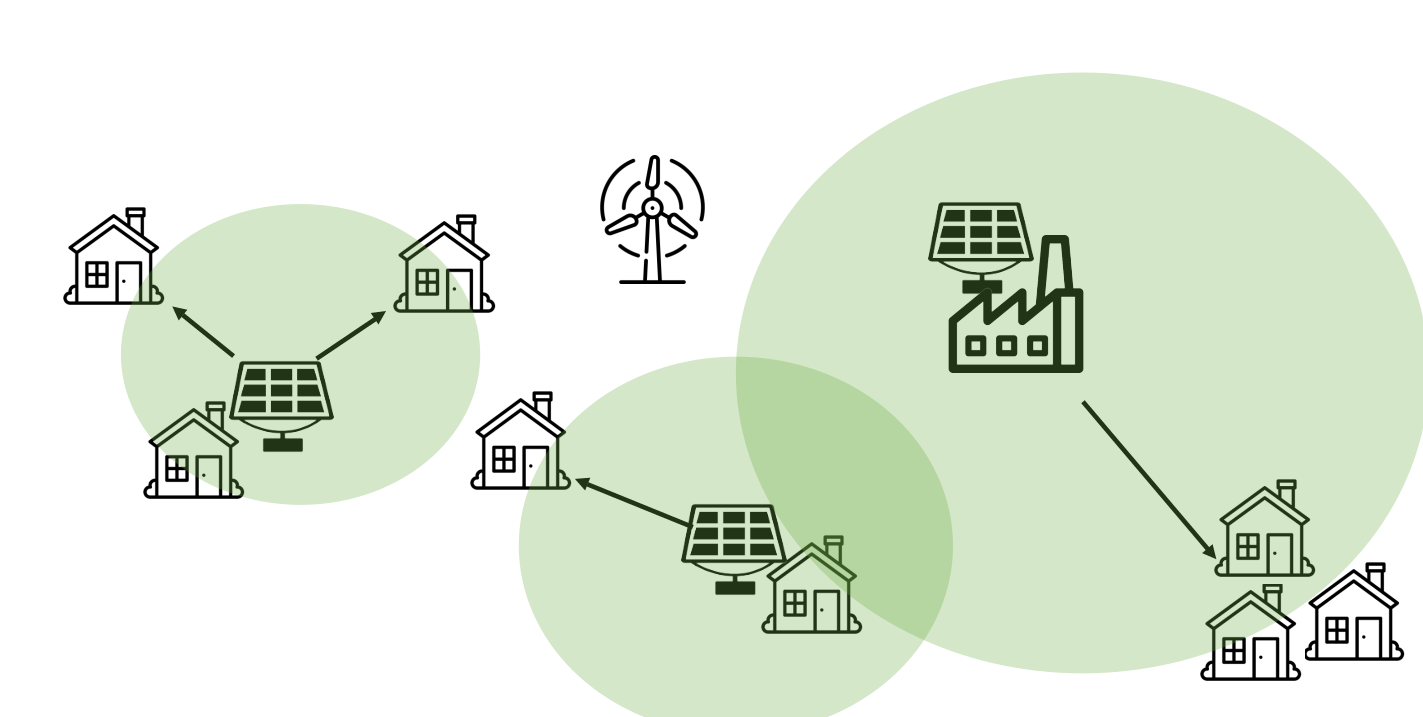
\includegraphics[width=11cm]{figs/huawei6}
  \end{center}
\end{frame}

\begin{frame}
  \frametitle{Futuro deseado}
  \begin{center}
    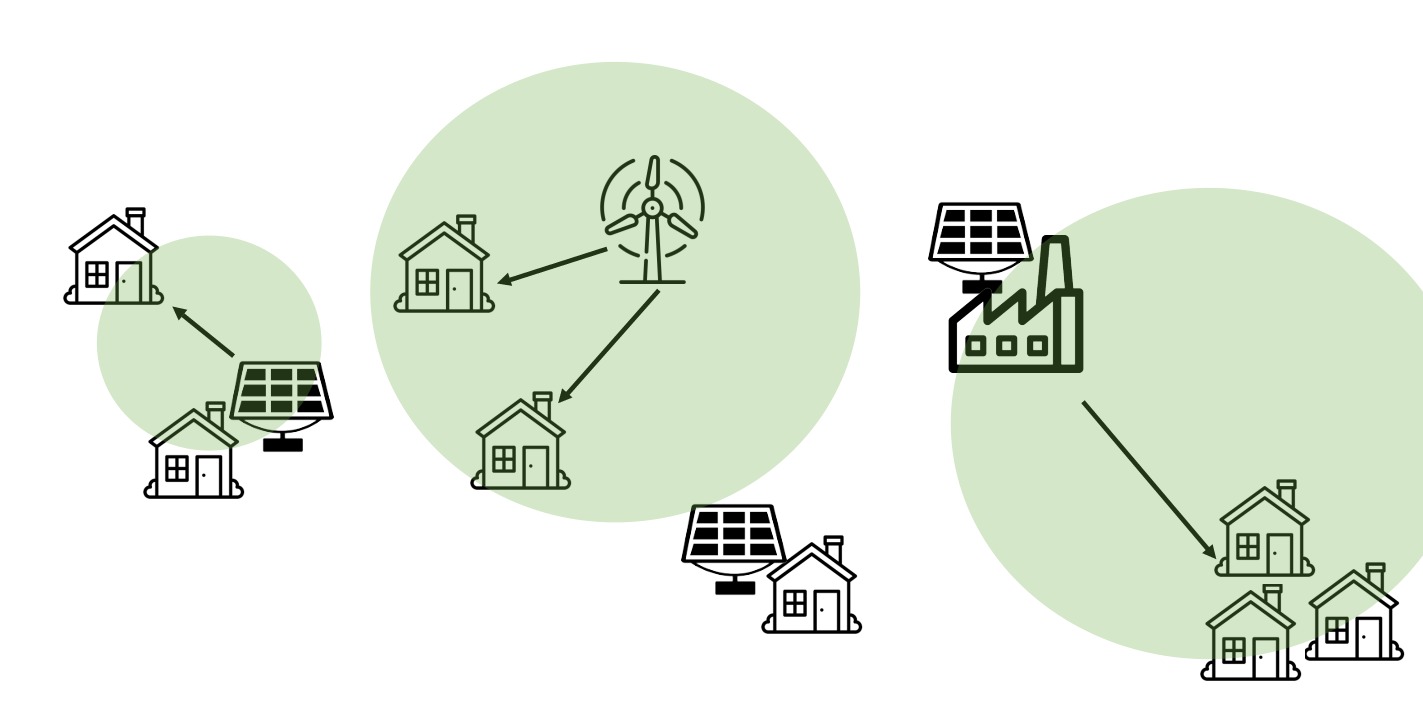
\includegraphics[width=11cm]{figs/huawei7}
  \end{center}
\end{frame}

\begin{frame}
  \frametitle{Futuro deseado}
  \begin{center}
    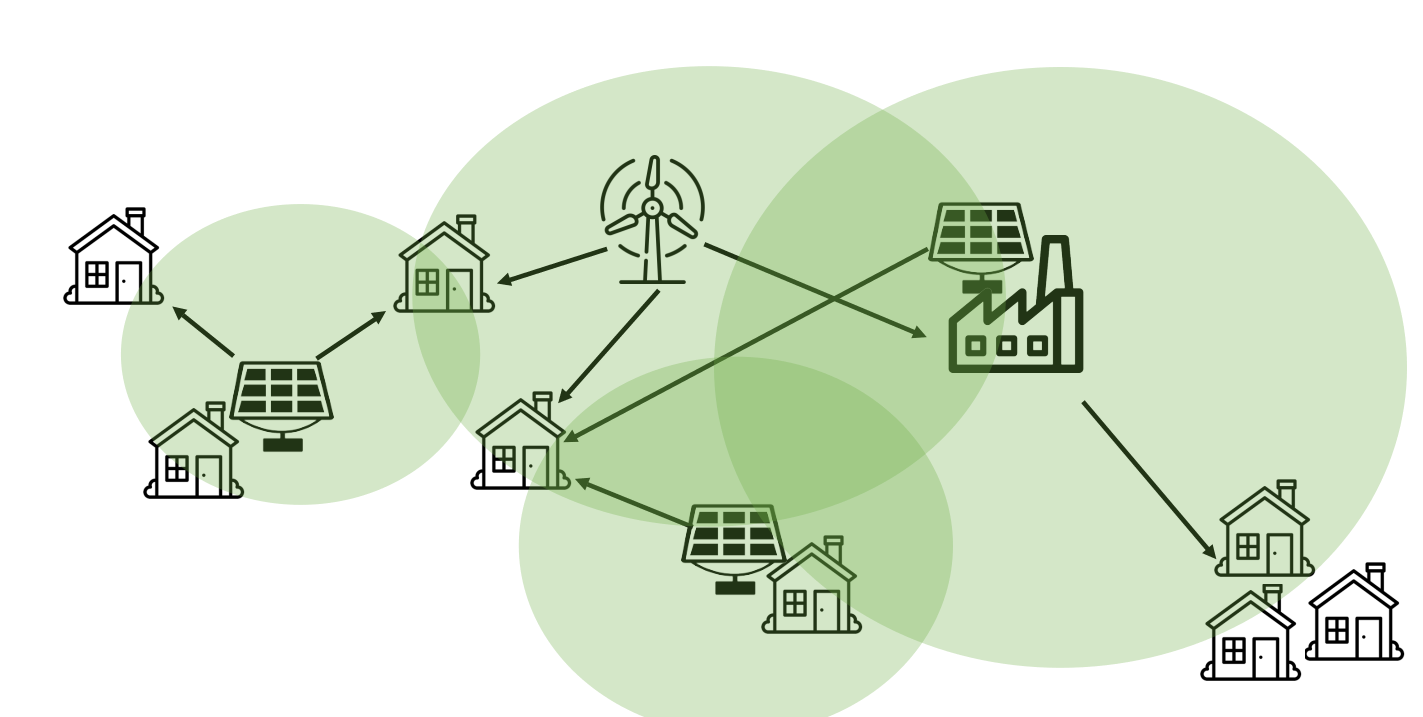
\includegraphics[width=11cm]{figs/huawei8}
  \end{center}
\end{frame}

\begin{frame}
  \frametitle{Motivación}
  \begin{center}	
    \includegraphics[width=11cm]{figs/gridGeneration_v2.eps}
    \vspace{0.2cm}
  \end{center}
  \begin{center}	
    {\Large \textbf{¿Cómo organizar?}} \\
    \vspace{0.2cm}
    {\Large\textbf{¿Cómo coordinar?}}\\
    \vspace{0.2cm}
    {\Large\textbf{¿Cómo autoadaptarse?}}
  \end{center}
\end{frame}

%------------%
\begin{frame}
  \frametitle{Insectos sociales}
	\begin{center}	
	  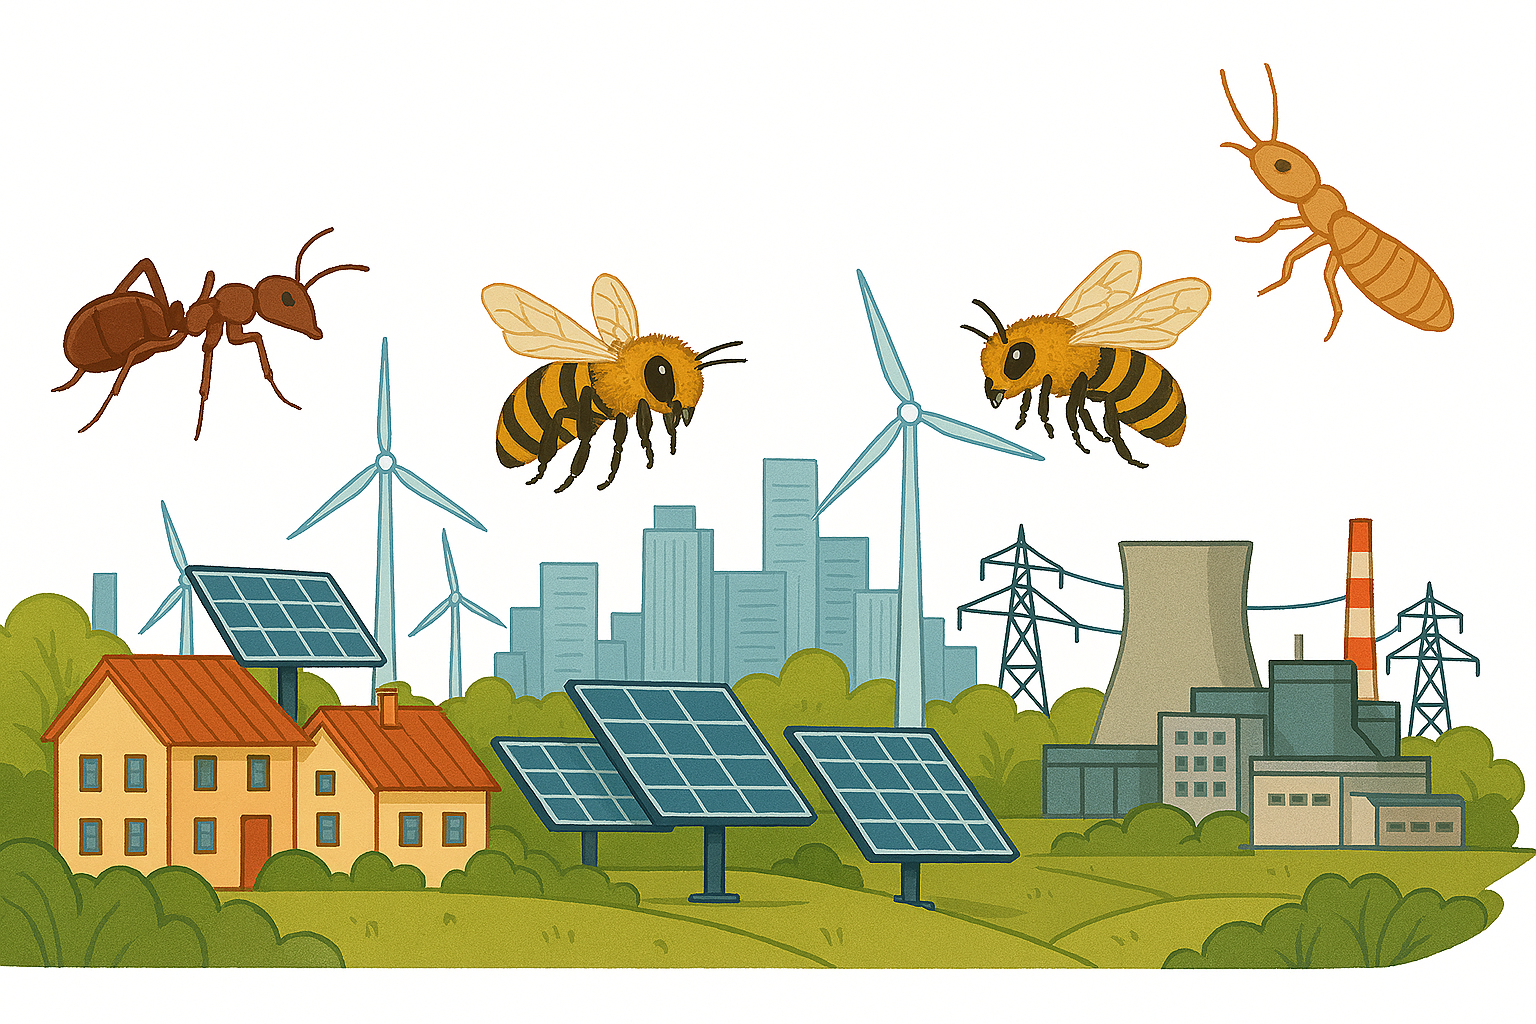
\includegraphics[width=10cm]{citySwarm_white}
	\end{center}
\end{frame}

%------------%
\begin{frame}
  \frametitle{Insectos sociales}
    \begin{center}
      \begin{tabular}{cc}
        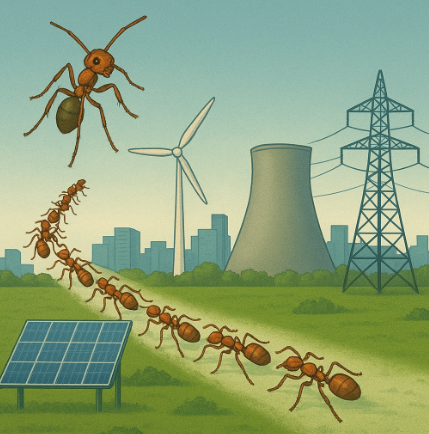
\includegraphics[width=4cm]{intro3} &
        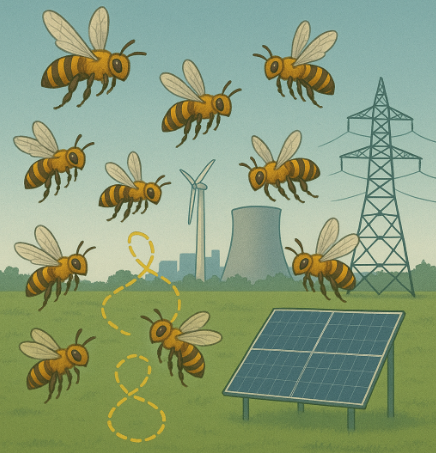
\includegraphics[width=3.9cm]{intro5} \\
      \end{tabular}
    \end{center}
  \begin{columns}
    \column{1.5cm}
    %\begin{center}	
      %%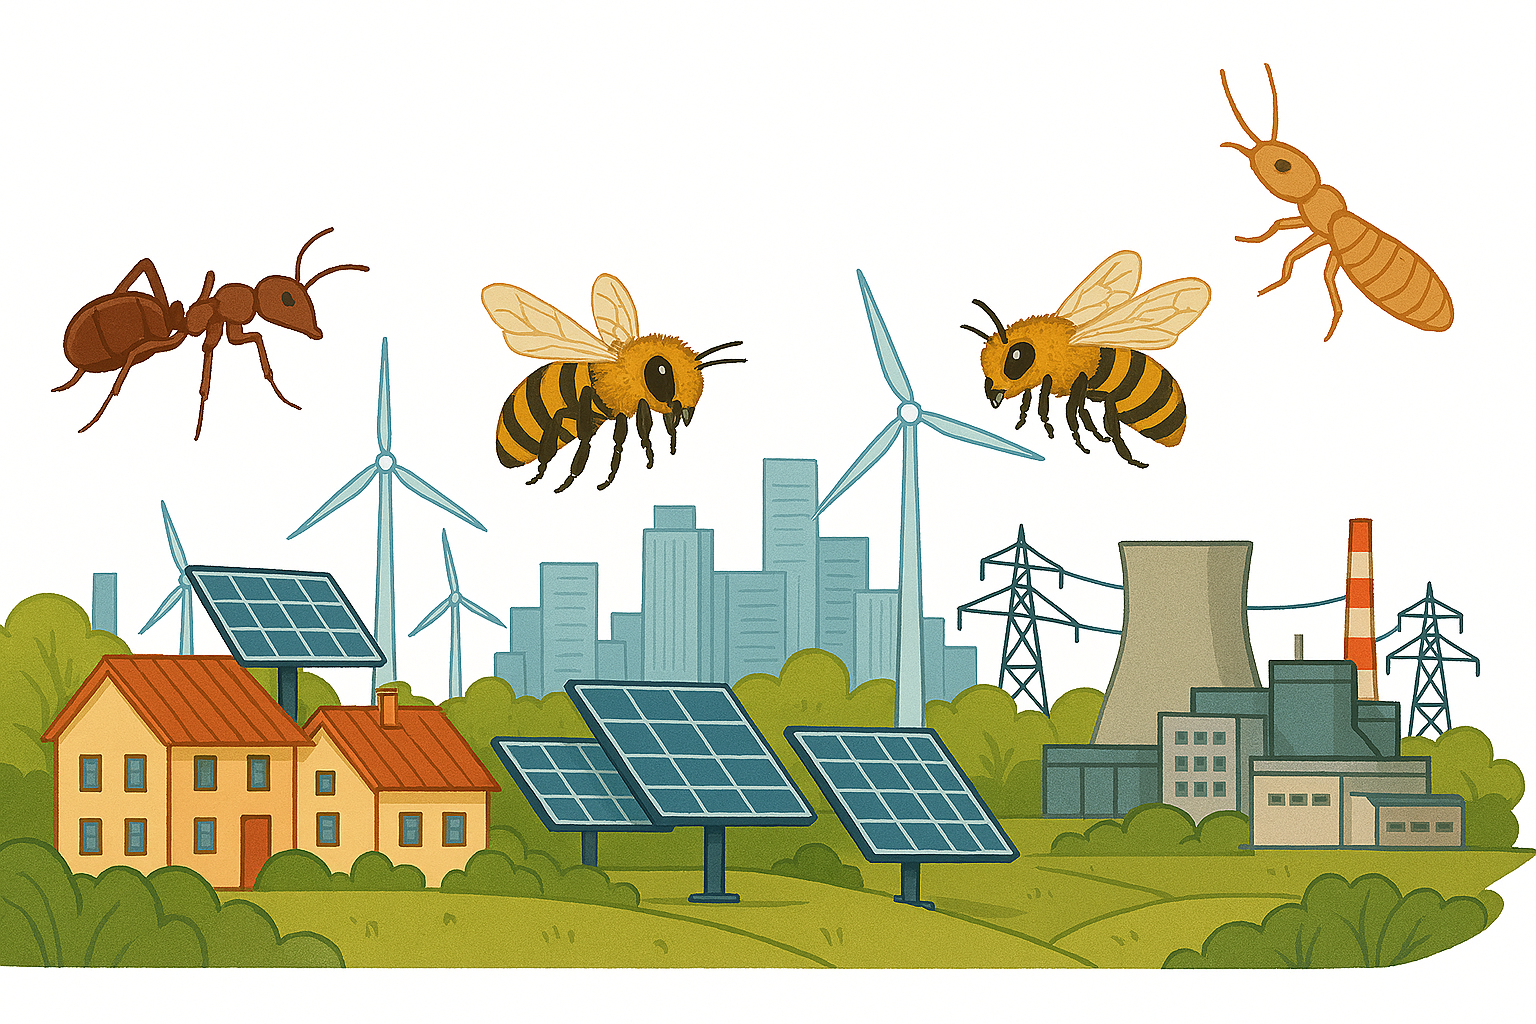
\includegraphics[width=5cm]{citySwarm_white}
    %%\end{center}
    \column{8cm}
    \begin{itemize}
      \item Control descentralizado
      \item Adaptación del colectivo
      \item Estigmergia (comunicación indirecta)
      \item Redundancia
      \item Eficiencia y optimización
    \end{itemize}
  %\end{center}
  \end{columns}
\end{frame}
%------------%

\begin{frame}
  \frametitle{Sociedades de insectos}
  \begin{center}
    \textbf{Control descentralizado}
  \end{center}
      \begin{itemize}
        \item \textbf{Sociedades de insectos}:
          \begin{itemize}
            \item Ningún insecto individual «dirige» la colonia
            \item Los individuos siguen reglas locales simples\\
            (rastros de feromonas, cambio de tareas,...)
            \item Surge un orden global
          \end{itemize}

        \item \textbf{Sistemas energéticos}: En las redes modernas,
          \begin{itemize}
            \item No existe un único controlador central para cada decisión\\
            \item Los dispositivos locales (paneles FV, baterías, contadores) actúan de forma autónoma \\
            según reglas simples (frecuencia, tensión, precio).
          \end{itemize}
      \end{itemize}
  %\end{itemize}
  \begin{center}
    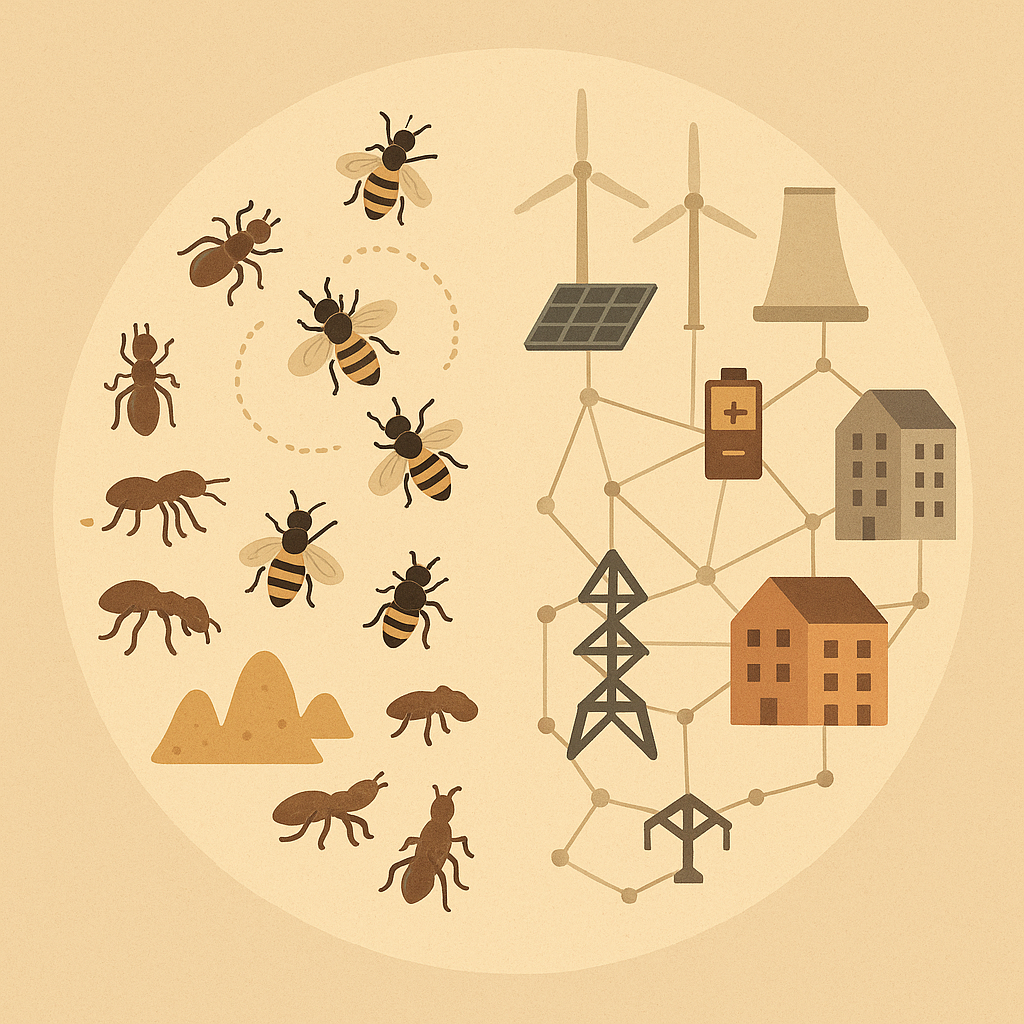
\includegraphics[width=3cm]{decentralizedInsects}
  \end{center}
\end{frame}

%------------%
\begin{frame}
  \frametitle{Sociedades de insectos}
  \begin{center}
    \textbf{Adaptación del colectivo}
  \end{center}

  \begin{itemize}
    \item \textbf{Sociedades de insectos}: los insectos redistribuyen el trabajo dinámicamente
      \begin{itemize}
        \item si hay abundancia de comida, más hormigas salen a recolectar
        \item si el nido es atacado, más insectos pasan a la defensa
      \end{itemize}
    \item \textbf{Sistemas energéticos}: los recursos se adaptan a las condiciones
      \begin{itemize}
        \item Se activa más almacenamiento cuando la generación renovable es alta
        \item Más respuesta de la demanda cuando el consumo aumenta
      \end{itemize}
  \end{itemize}
  
  \begin{center}
    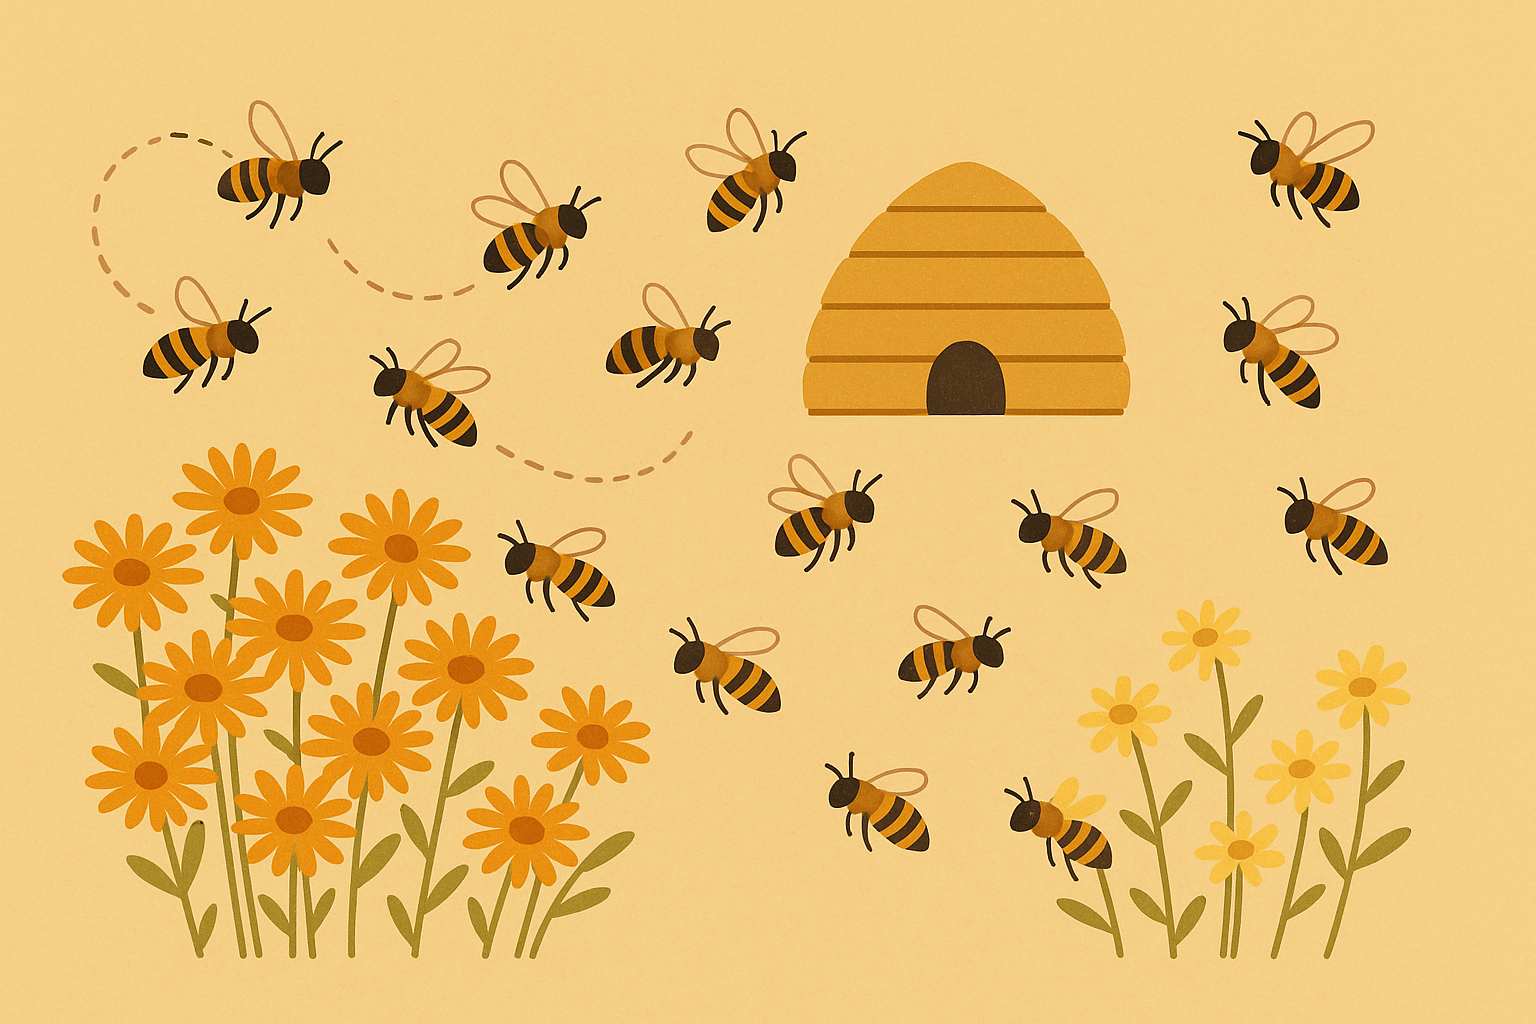
\includegraphics[width=5cm]{adaptationInsects}
  \end{center}
\end{frame}

%------------%
\begin{frame}
  \frametitle{Sociedades de insectos}
  \begin{center}
    \textbf{Estigmergia (comunicación indirecta)}
  \end{center}

      \begin{itemize}
        \item \textbf{Sociedades de insectos}:
          \begin{itemize}
                \item Las hormigas usan rastros de feromonas
                \item las termitas construyen grandes nidos respondiendo a cambios locales
                \item No se requiere comunicación directa.
          \end{itemize}

        \item \textbf{Sistemas energéticos}: los dispositivos de una red a menudo reaccionan de forma indirecta
          \begin{itemize}
            \item Las caídas de frecuencia indican a los generadores que aumenten su producción
            \item las señales de precio coordinan el consumo o la generación
          \end{itemize}
      \end{itemize}
  \begin{center}
    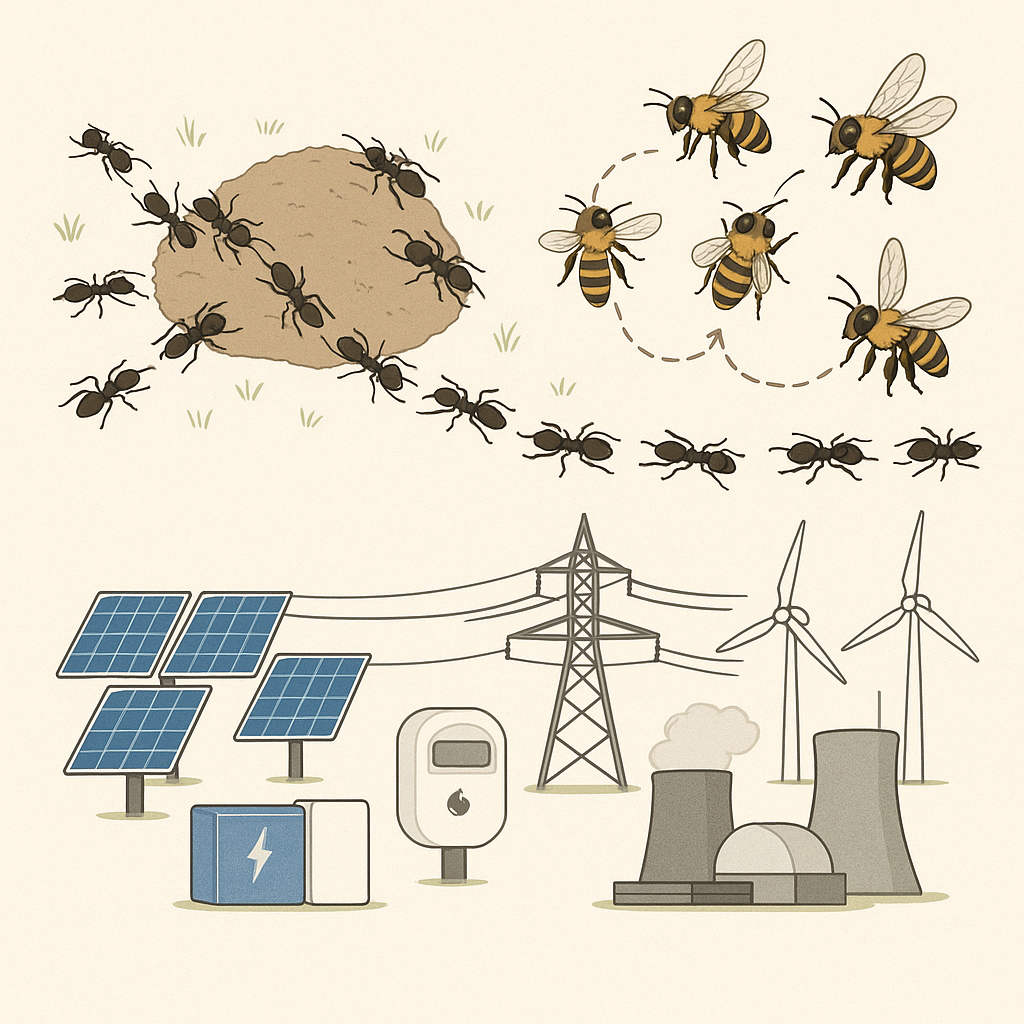
\includegraphics[width=4cm]{stigmergyInsects}
  \end{center}
\end{frame}

%------------%
\begin{frame}
  \frametitle{Sociedades de insectos}
  \begin{center}
    \textbf{Redundancia}
  \end{center}

      \begin{itemize}
        \item \textbf{Sociedades de insectos}:
          \begin{itemize}
            \item Las colonias sobreviven aunque mueran insectos individuales, \\
              porque las funciones están distribuidas y son redundantes.
          \end{itemize}
        \item \textbf{Sistemas energéticos}:
          \begin{itemize}
            \item Una red con muchos recursos distribuidos (FV, VE, baterías) \\
              debe seguir funcionando aunque falle una (o varias) planta.
      \end{itemize}
  \end{itemize}
  \begin{center}
    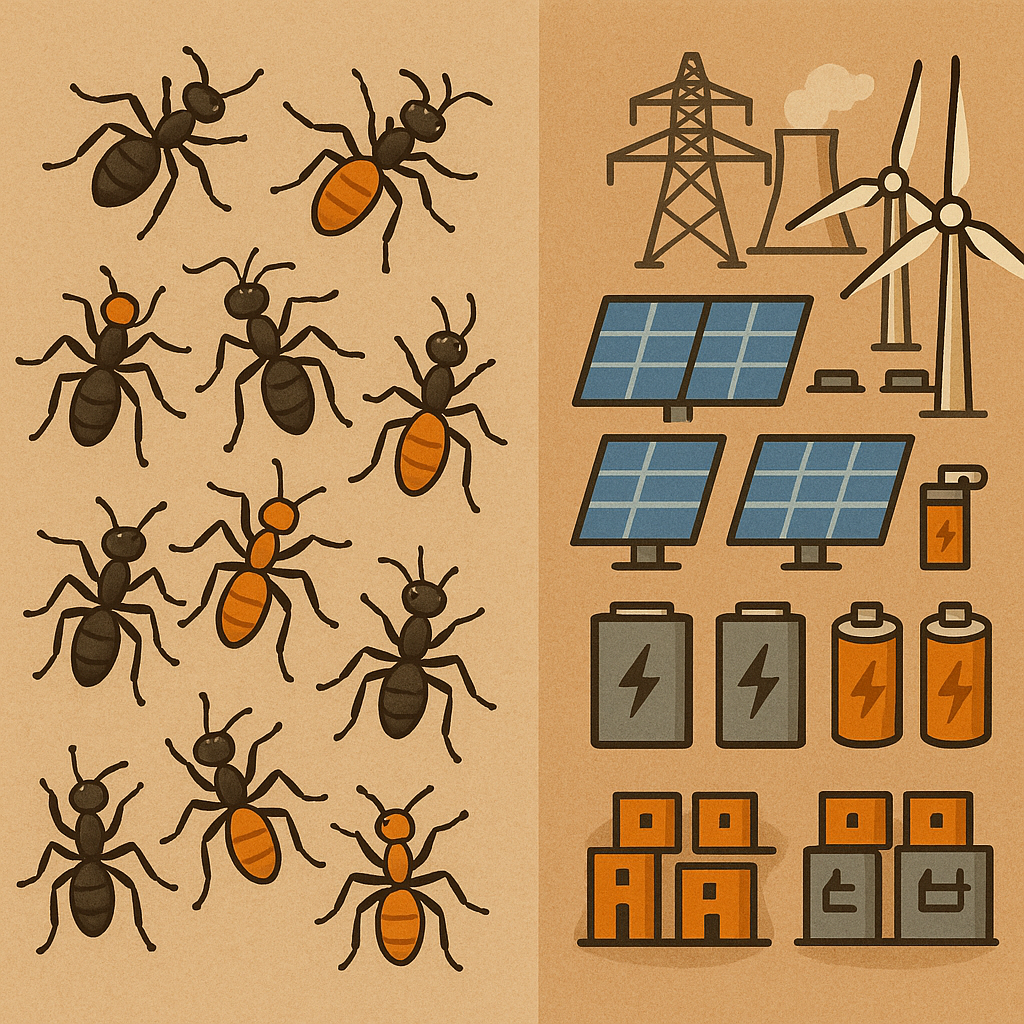
\includegraphics[width=4cm]{redundancyInsects}
  \end{center}
\end{frame}

%------------%
\begin{frame}
  \frametitle{Sociedades de insectos}
  \begin{center}
    \textbf{Eficiencia y optimización}
  \end{center}

      \begin{itemize}
        \item \textbf{Sociedades de insectos}:
          \begin{itemize}
            \item Las colonias de hormigas encuentran rutas casi óptimas hacia la comida, \\
              equilibrando exploración y explotación.
          \end{itemize}

        \item \textbf{Sistemas energéticos}:
          \begin{itemize}
            \item Se usan algoritmos de enrutamiento para optimizar la planificación de los flujos de potencia y las rutas de energía.
      \end{itemize}
  \end{itemize}
  \begin{center}
    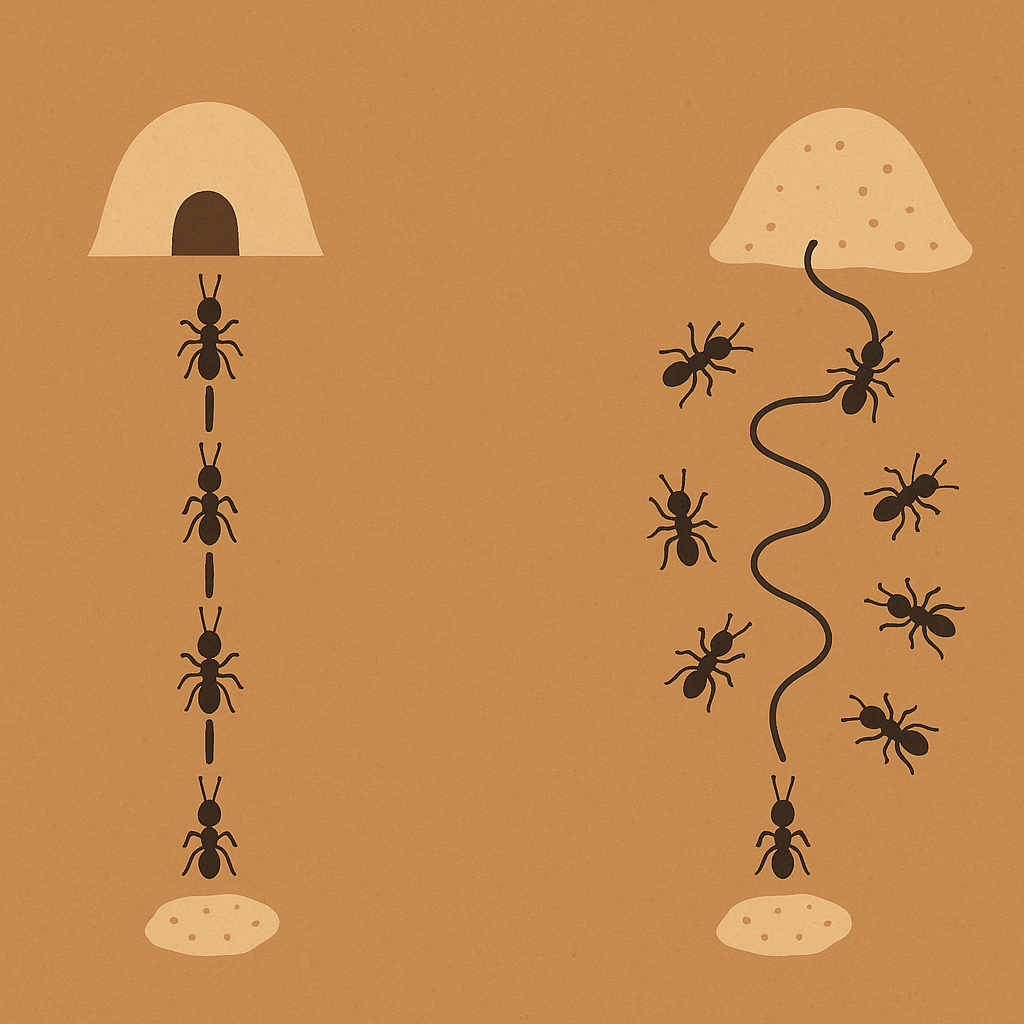
\includegraphics[width=4cm]{optimizationInsects}
  \end{center}
\end{frame}

\begin{frame}
  \frametitle{Insectos sociales}
	\begin{center}	
    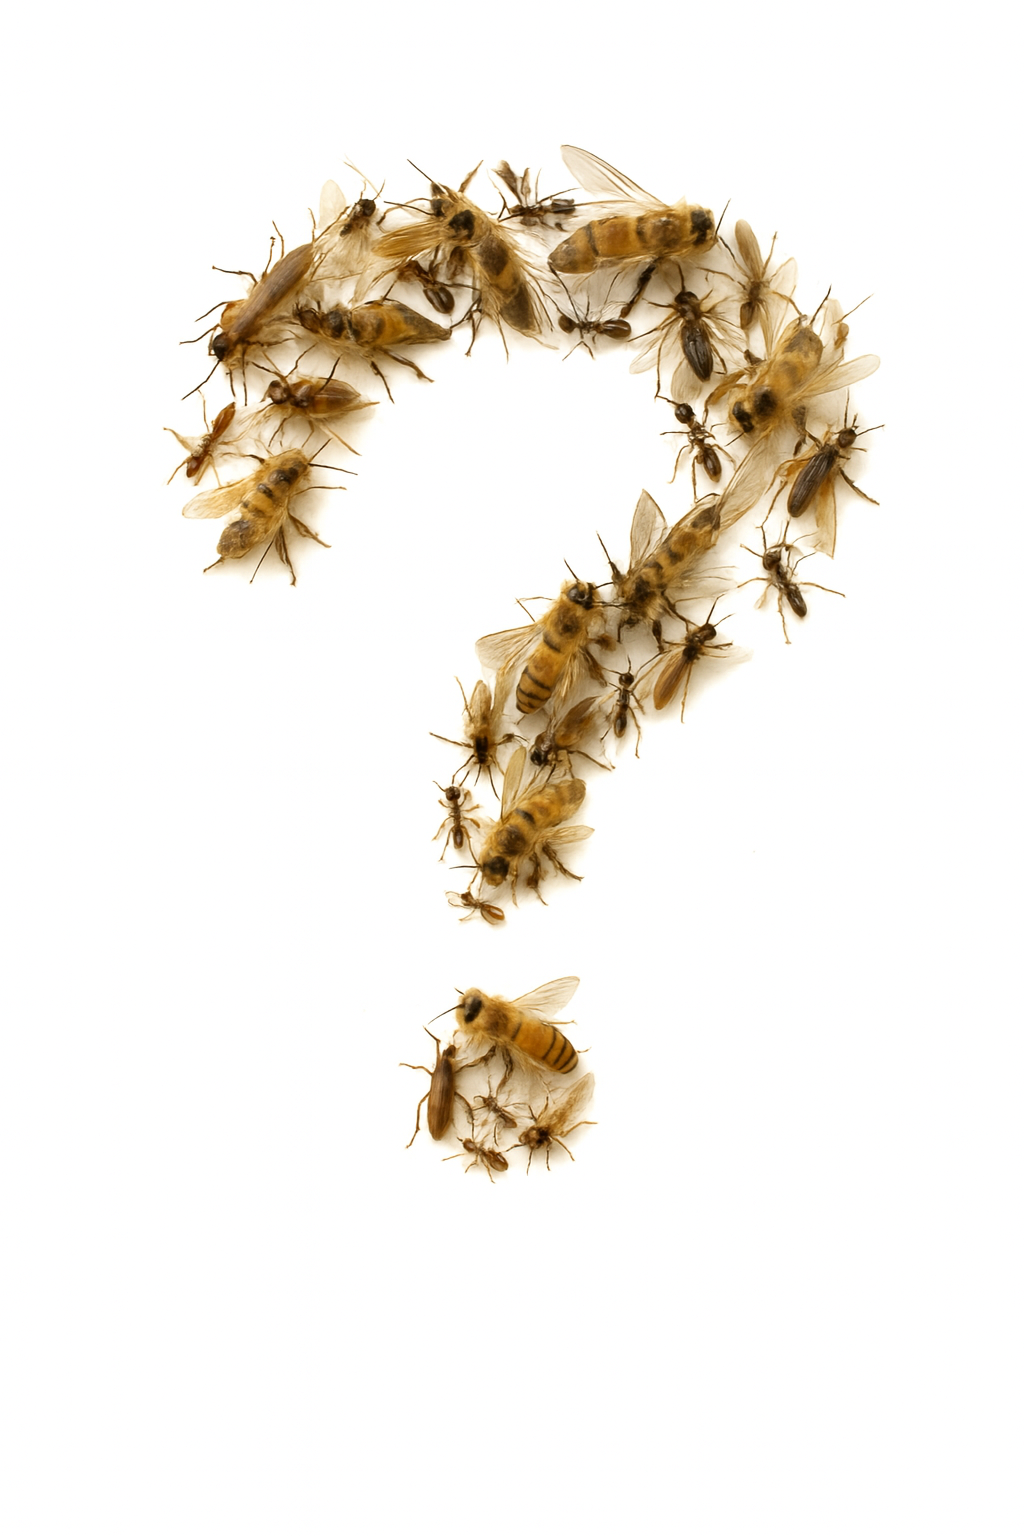
\includegraphics[width=5cm]{questionMarkInsects_white}
	\end{center}
\end{frame}

%------------%
%------------%
\begin{frame}
  \frametitle{Modelo de prueba}
	\begin{center}
    \begin{tabular}{cc}
	  \includegraphics[width=4.5cm]{magicbox.eps} 
	  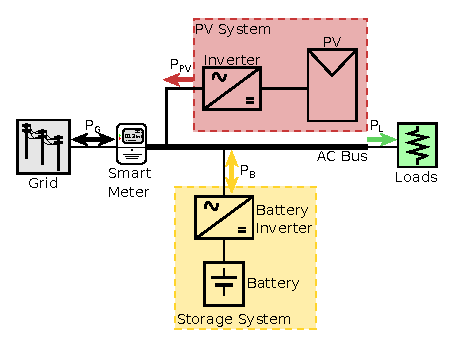
\includegraphics[width=6cm]{electricDiagram0.eps} 
    \end{tabular}
	\end{center}
\end{frame}

%------------%
\begin{frame}
  \frametitle{Estigmergia}

	\begin{center}
    \begin{tabular}{cc}
      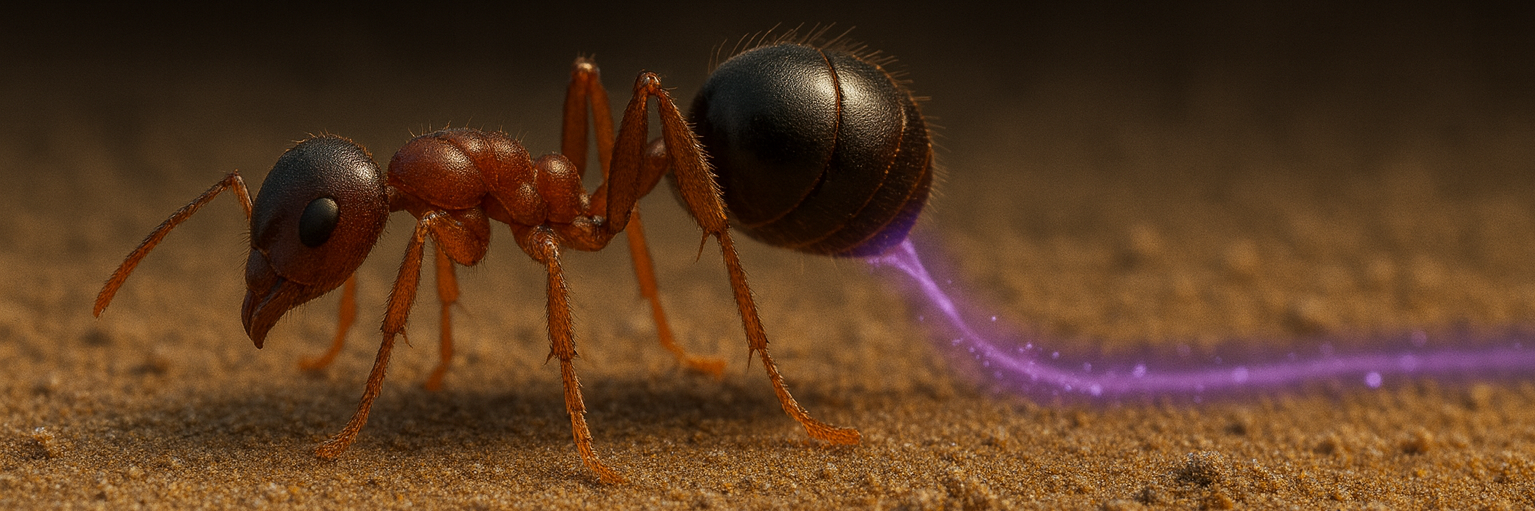
\includegraphics[width=5cm]{figs/antsTrail3}&
      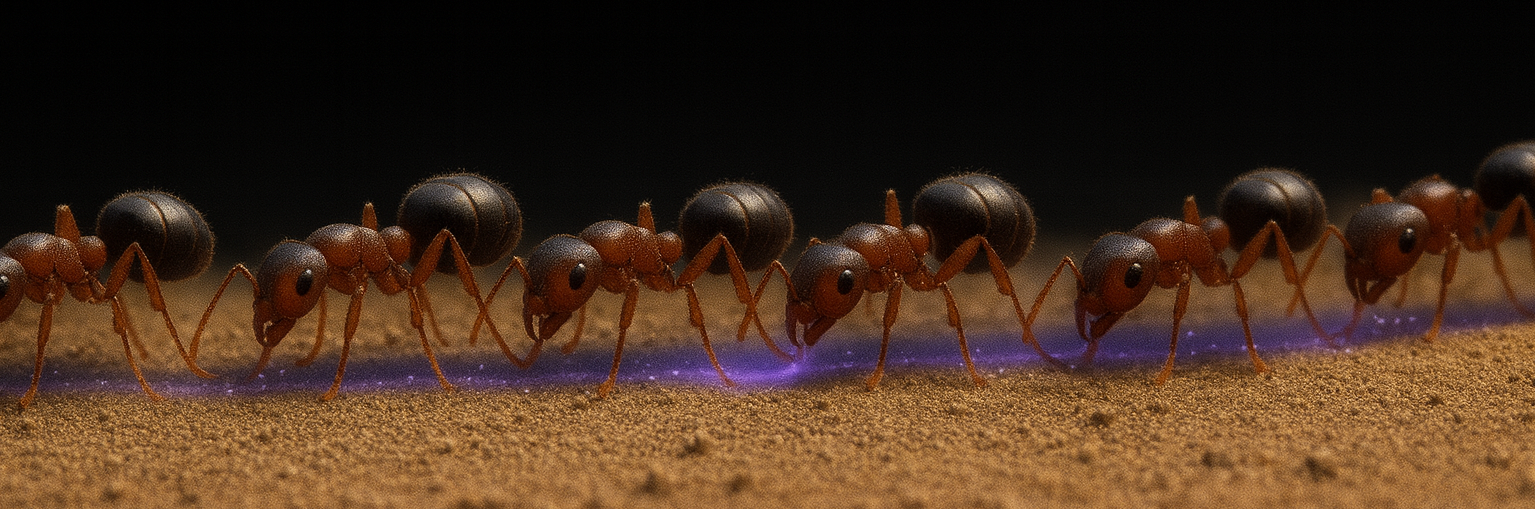
\includegraphics[width=5cm]{figs/antsTrail4}\\
    \end{tabular}

  \end{center}
		\vspace{0.4cm}
    \begin{center}
      \includegraphics<1>[width=7cm]{figs/antsTrail7}
      \includegraphics<2>[width=10cm]{figs/casasStigmergy.eps}
    \end{center}
\end{frame}

\begin{frame}
  \frametitle{División del trabajo}

	\begin{center}
    \begin{tikzpicture}
      \node [inner sep=0pt] at (0,0) {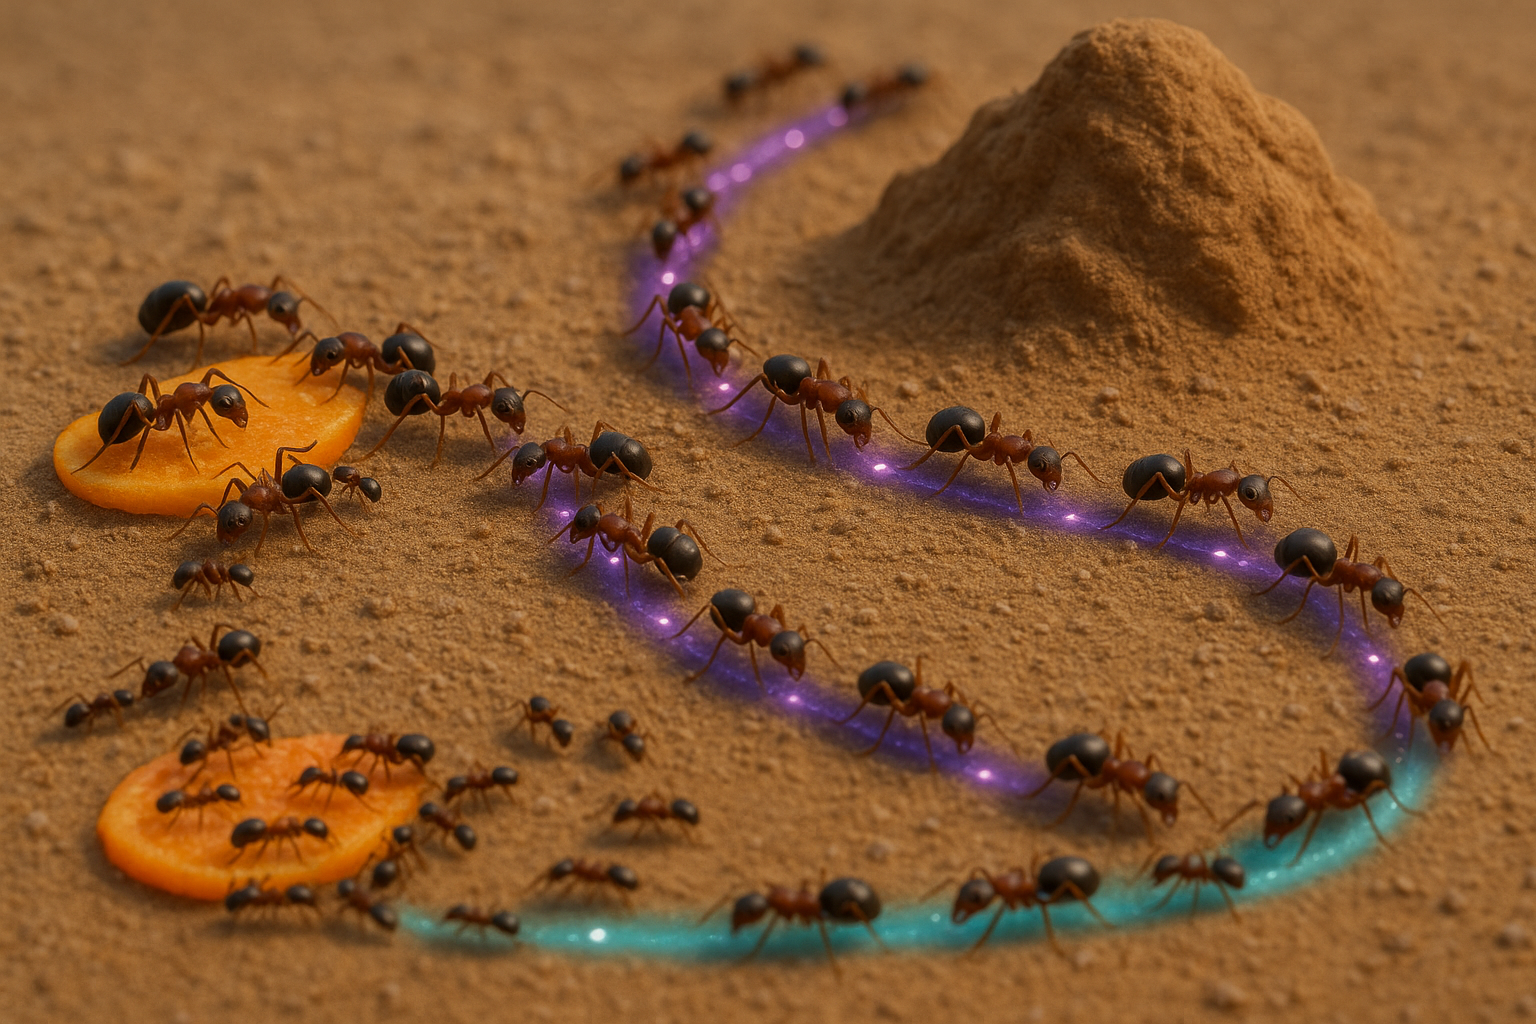
\includegraphics[width=4.5cm]{figs/AntsDivisionOfLabor}};
      \draw [white, rounded corners=\ClipSep, line width=\ClipSep] 
      (current bounding box.north west) -- 
      (current bounding box.north east) --
      (current bounding box.south east) --
      (current bounding box.south west) -- cycle
      ;
    \end{tikzpicture}
    \begin{tikzpicture}
      \node [inner sep=0pt] at (0,0) {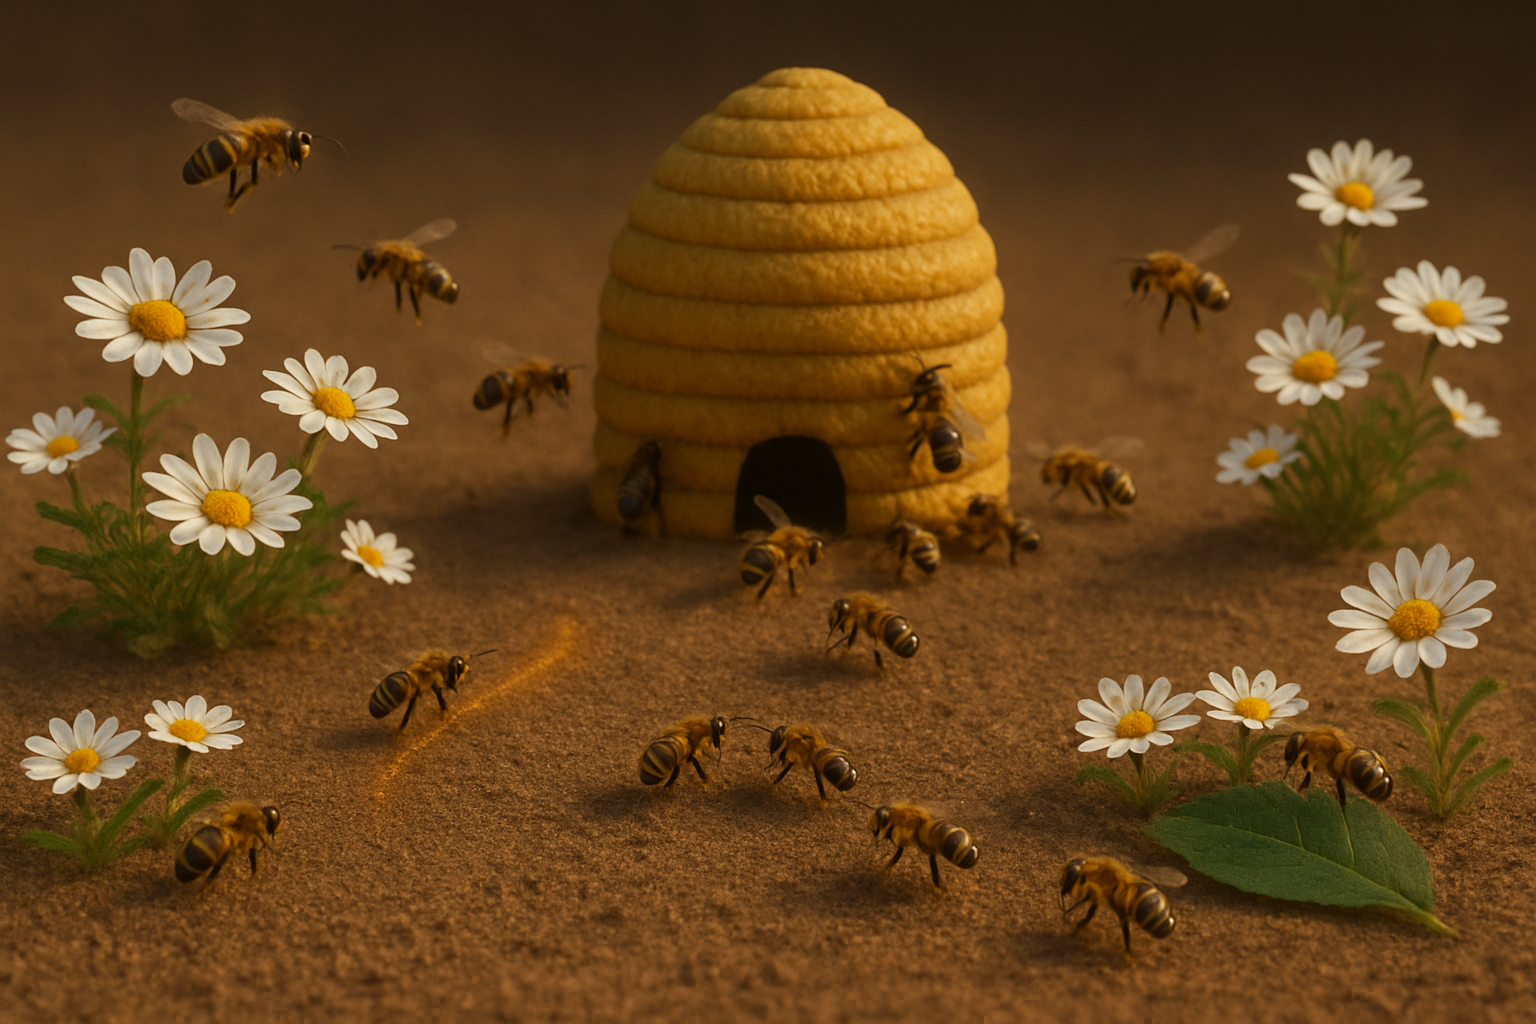
\includegraphics[width=4.5cm]{figs/BeesDivisionOfLabor}};
      \draw [white, rounded corners=\ClipSep, line width=\ClipSep] 
      (current bounding box.north west) -- 
      (current bounding box.north east) --
      (current bounding box.south east) --
      (current bounding box.south west) -- cycle
      ;
    \end{tikzpicture}
		\vspace{0.75cm}
	\pause	
		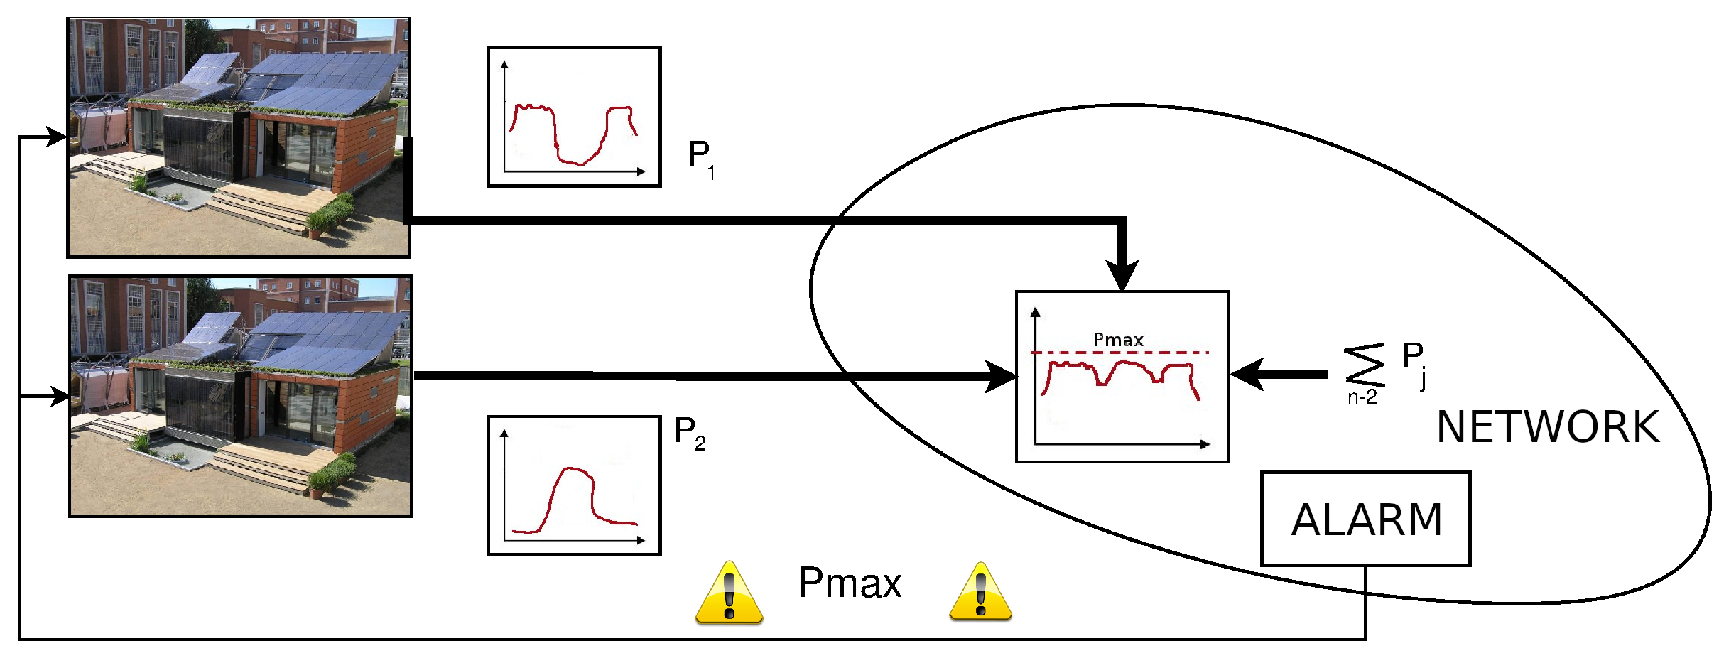
\includegraphics[width=10cm]{figs/casasDivision.eps}
		
	\end{center}
\end{frame}

\begin{frame}
	\frametitle{Construcción del nido}
	
	\begin{center}
		%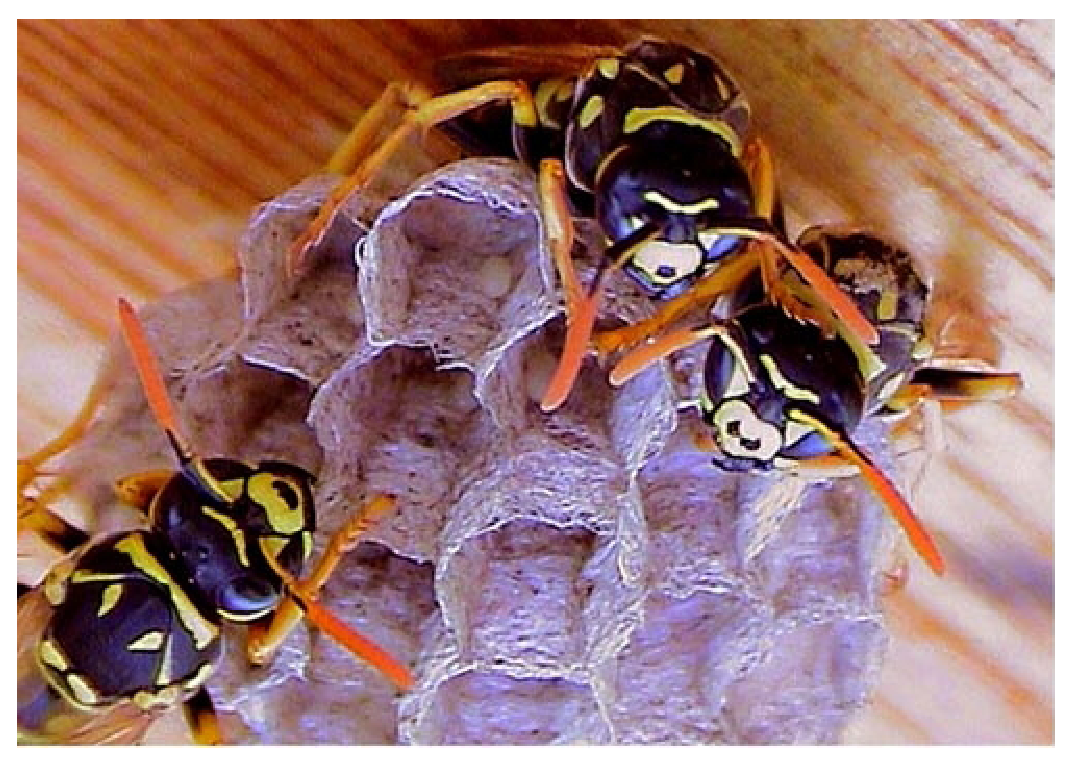
\includegraphics[width=3cm]{figs/waspNest.eps} \hspace{0.5cm}
		%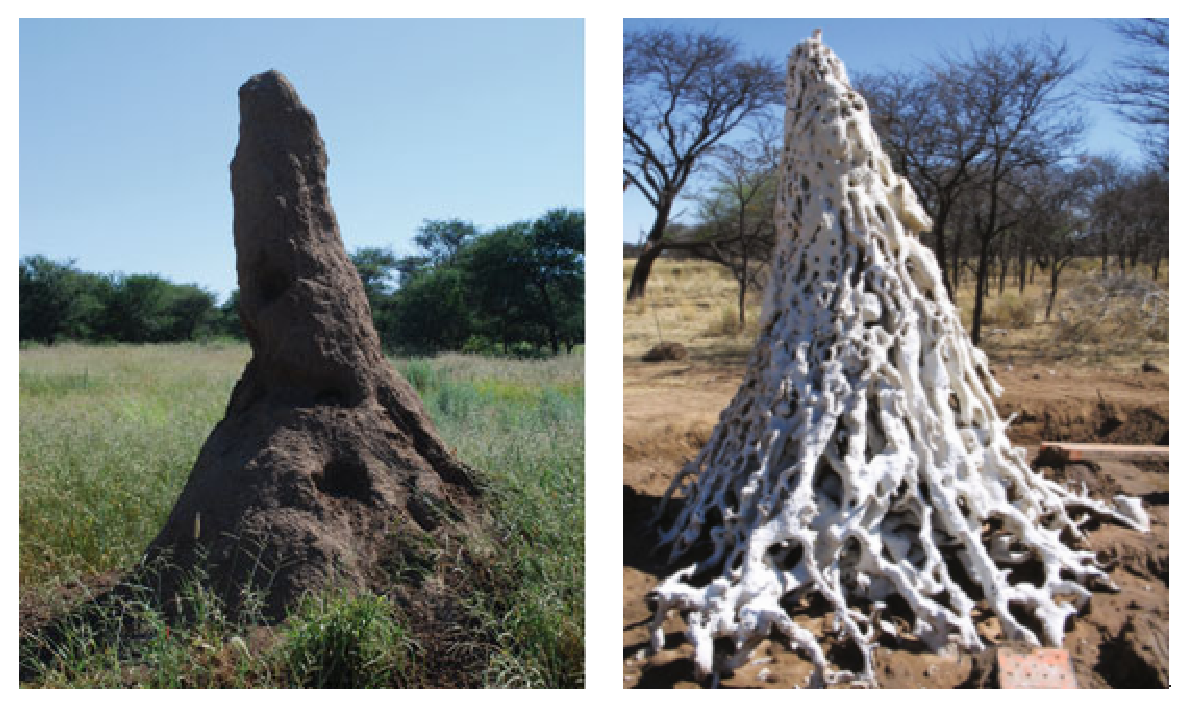
\includegraphics[width=4cm]{figs/termitesNest.eps}
    \begin{tikzpicture}
      \node [inner sep=0pt] at (0,0) {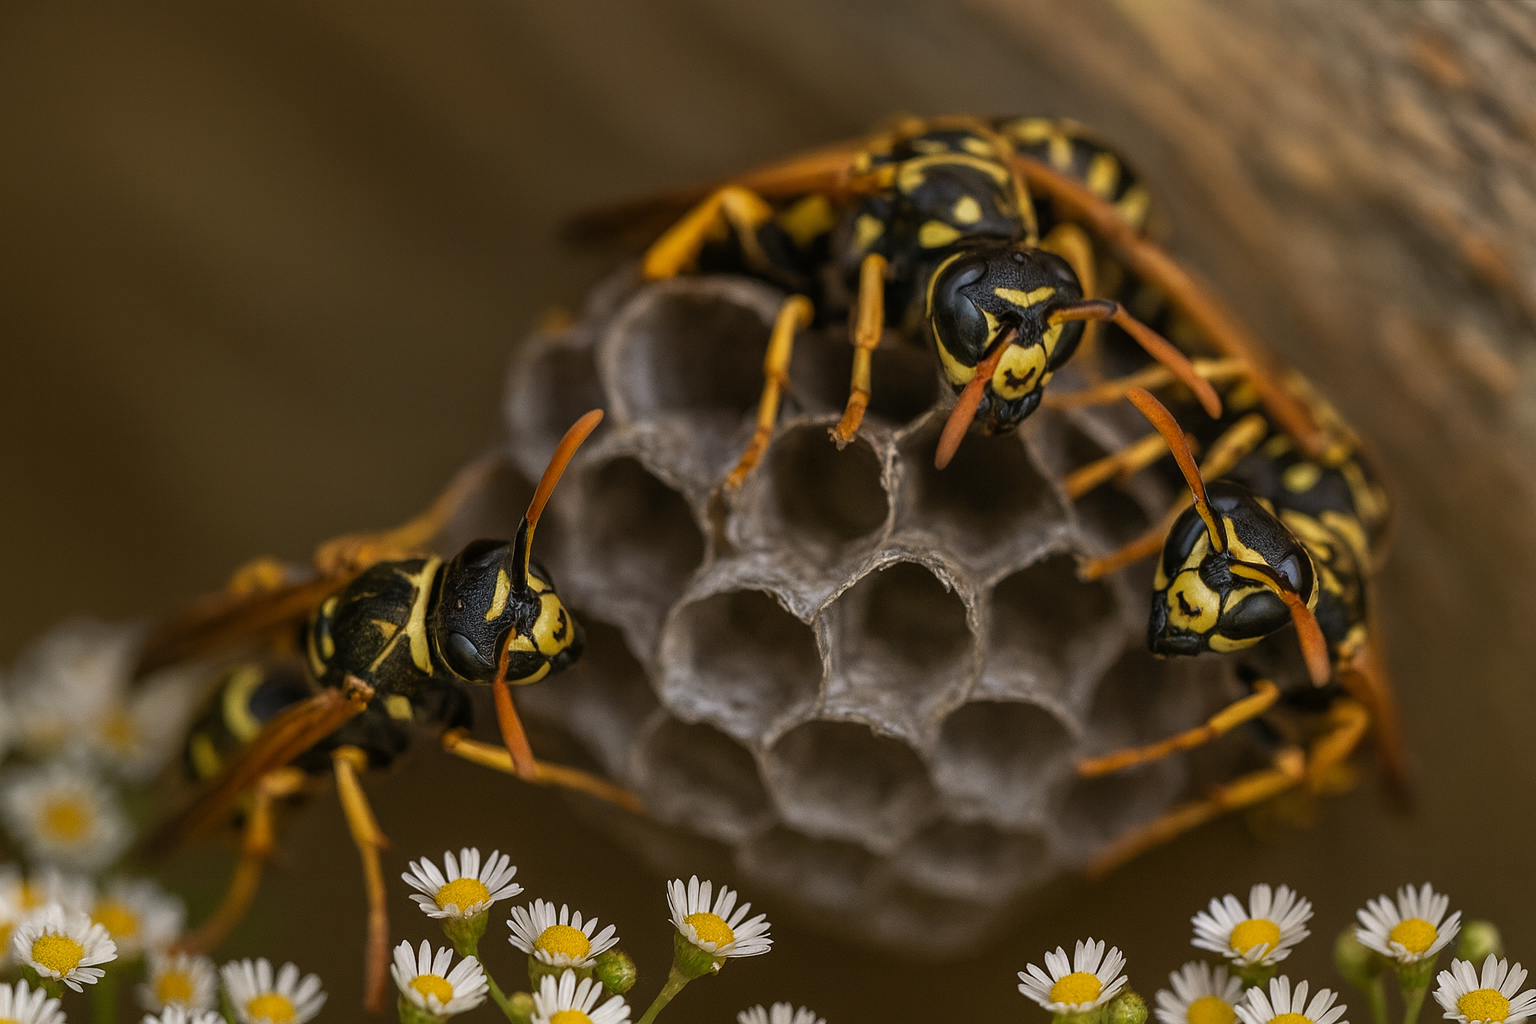
\includegraphics[width=4.5cm]{figs/WaspsNests}};
      \draw [white, rounded corners=\ClipSep, line width=\ClipSep] 
      (current bounding box.north west) -- 
      (current bounding box.north east) --
      (current bounding box.south east) --
      (current bounding box.south west) -- cycle
      ;
    \end{tikzpicture}
    \begin{tikzpicture}
      \node [inner sep=0pt] at (0,0) {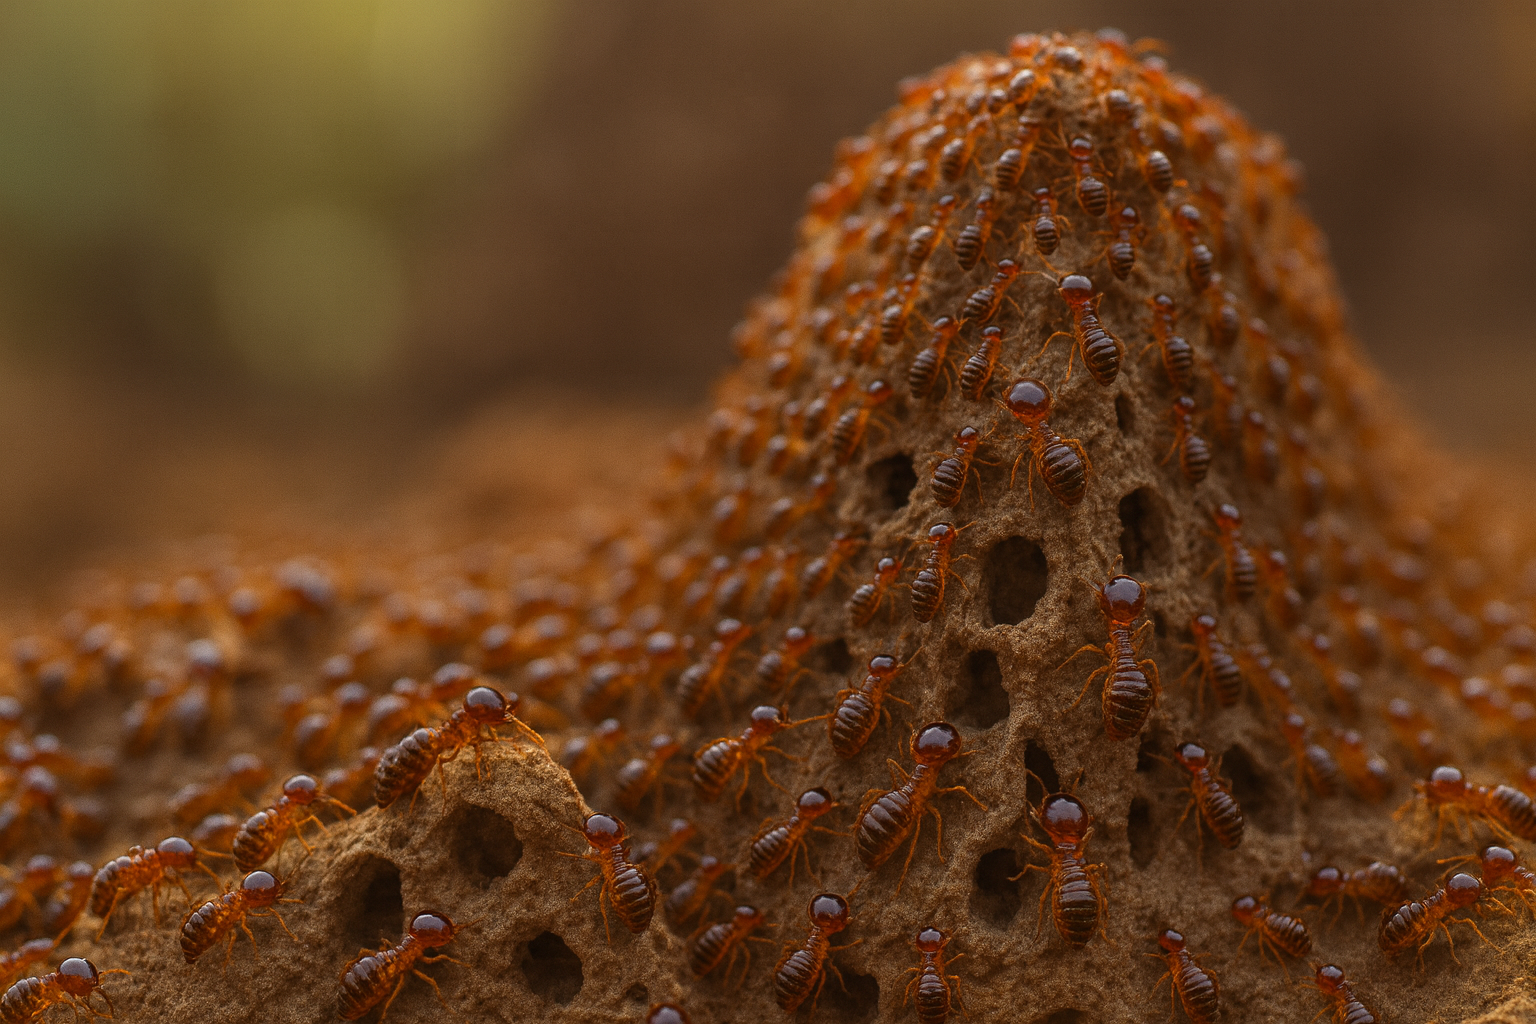
\includegraphics[width=4.5cm]{figs/ThermitesNests}};
      \draw [white, rounded corners=\ClipSep, line width=\ClipSep] 
      (current bounding box.north west) -- 
      (current bounding box.north east) --
      (current bounding box.south east) --
      (current bounding box.south west) -- cycle
      ;
    \end{tikzpicture}
		\vspace{0.5cm}
		
		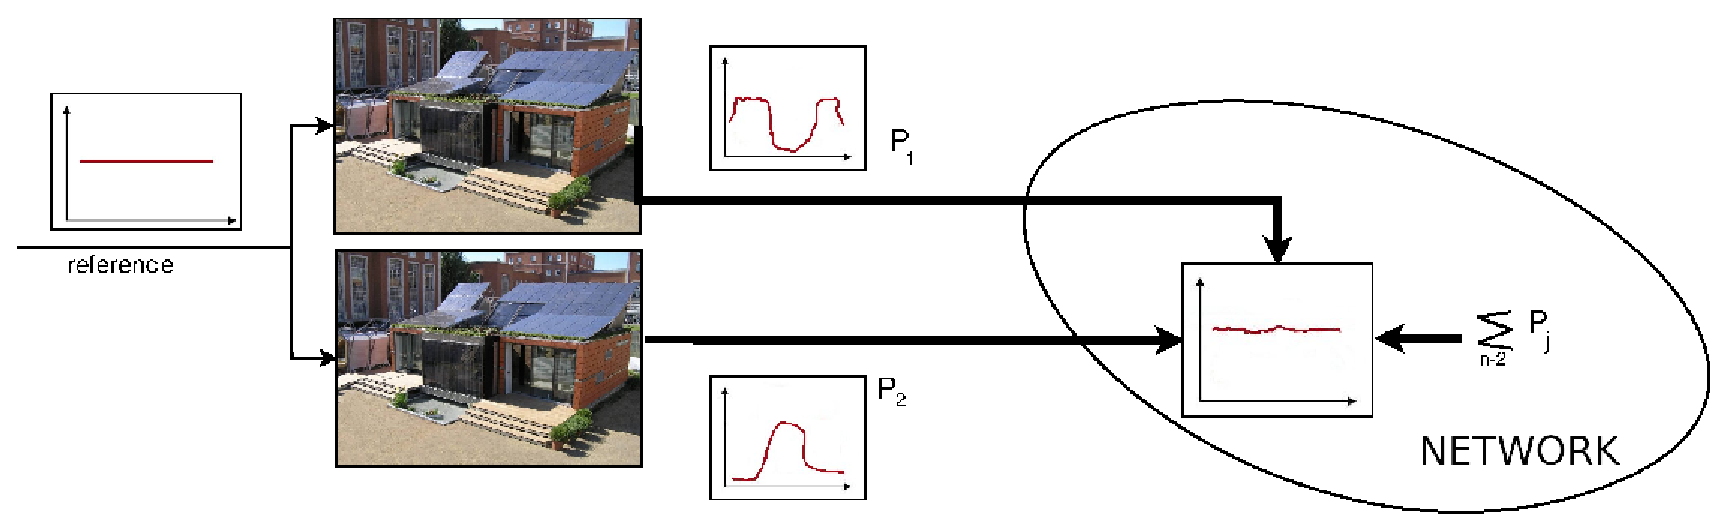
\includegraphics[width=11cm]{figs/casasNest.eps}
		
	\end{center}
\end{frame}

\begin{frame}
	\frametitle{Gestión de la Demanda (DSM)}
	\begin{center}
		$P(t) = P^{nc}(t) + P^{c}(t)$
	\end{center}
	\vspace{0.5cm}
	\begin{columns}
	\column{6cm}		
		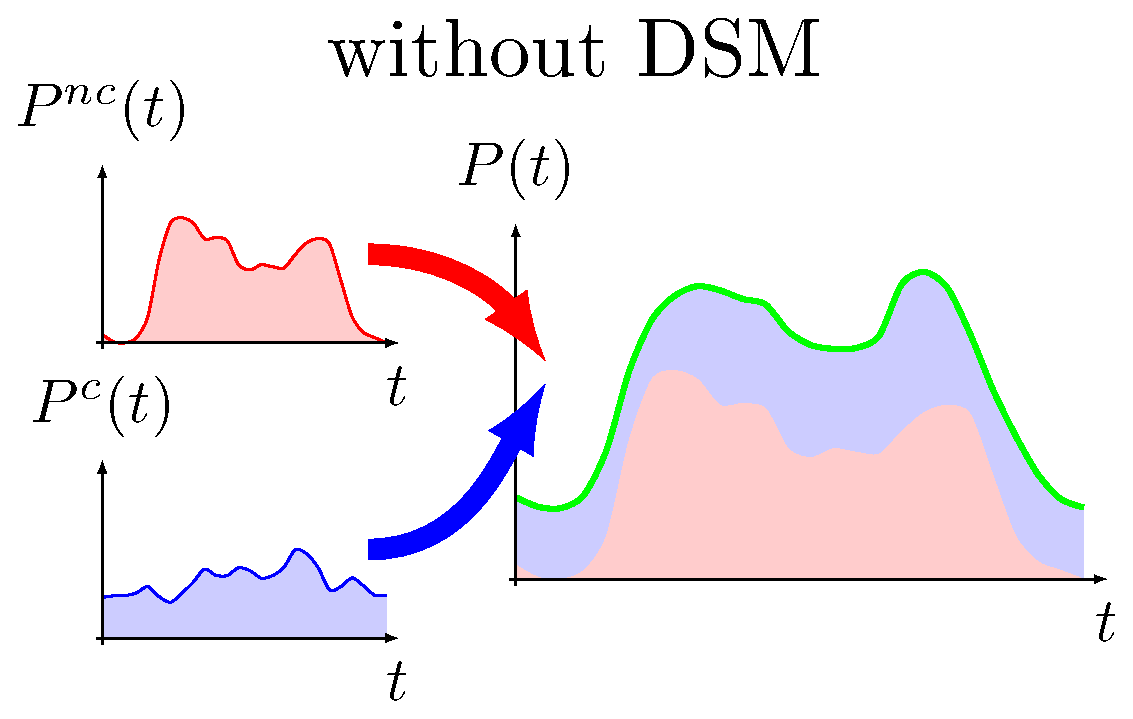
\includegraphics[width=6cm]{figs/signal_rep_initial.eps}
	\column{6cm}	
		\includegraphics<2>[width=6cm]{figs/signal_rep_final.eps}
	\end{columns}
\end{frame}

%%------------%
\begin{frame}
	\begin{center}
    \frametitle{Consumo agregado}
	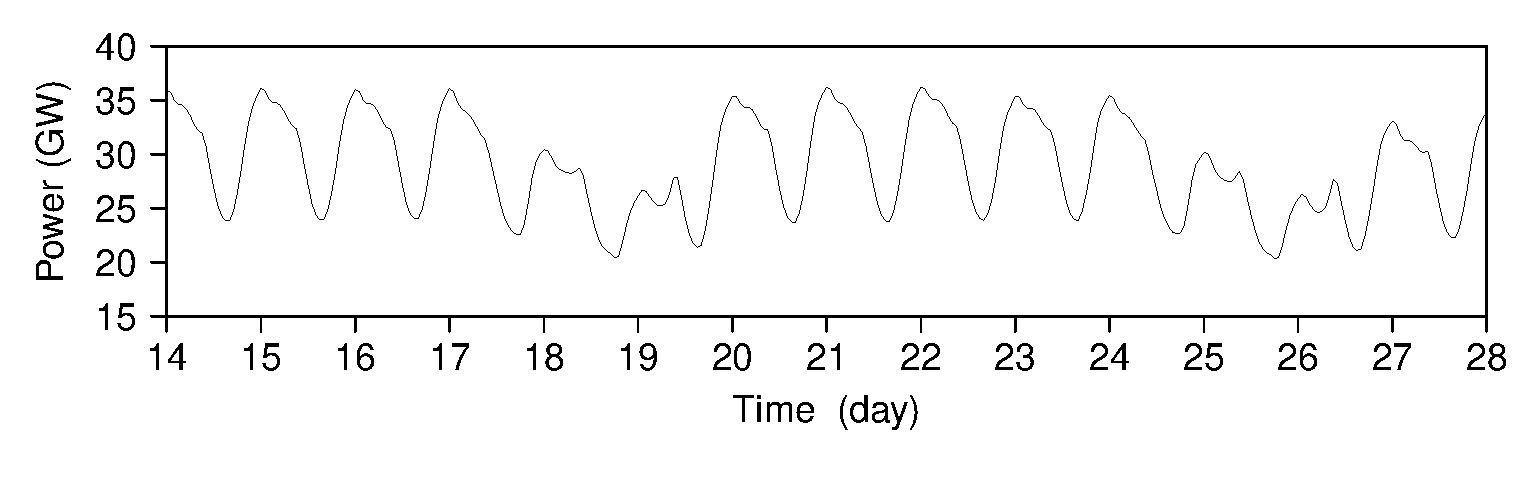
\includegraphics[width=11cm]{figs/plot_mufco_grid_nosc_week.eps}\\
	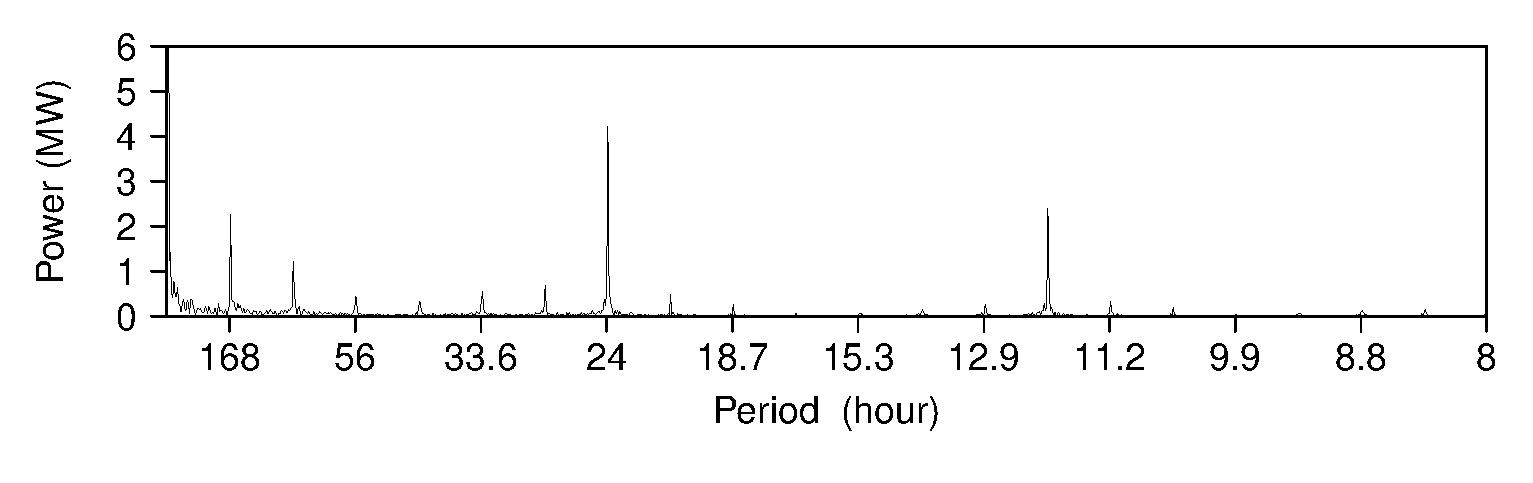
\includegraphics[width=11cm]{figs/plot_mufco_grid_nosc_fft.eps}
	\end{center}
\end{frame}
%------------%
%\begin{frame}
	%\frametitle{Frequency development}
	%\begin{center}
    %%{\bf Serie de fourier} $\rightarrow$
	%$P(t)      = \sum\limits_{n=1}^{N} A_{n} sin ( n \omega_{0} t + \phi_{n} ) + e(t)$ \\
	%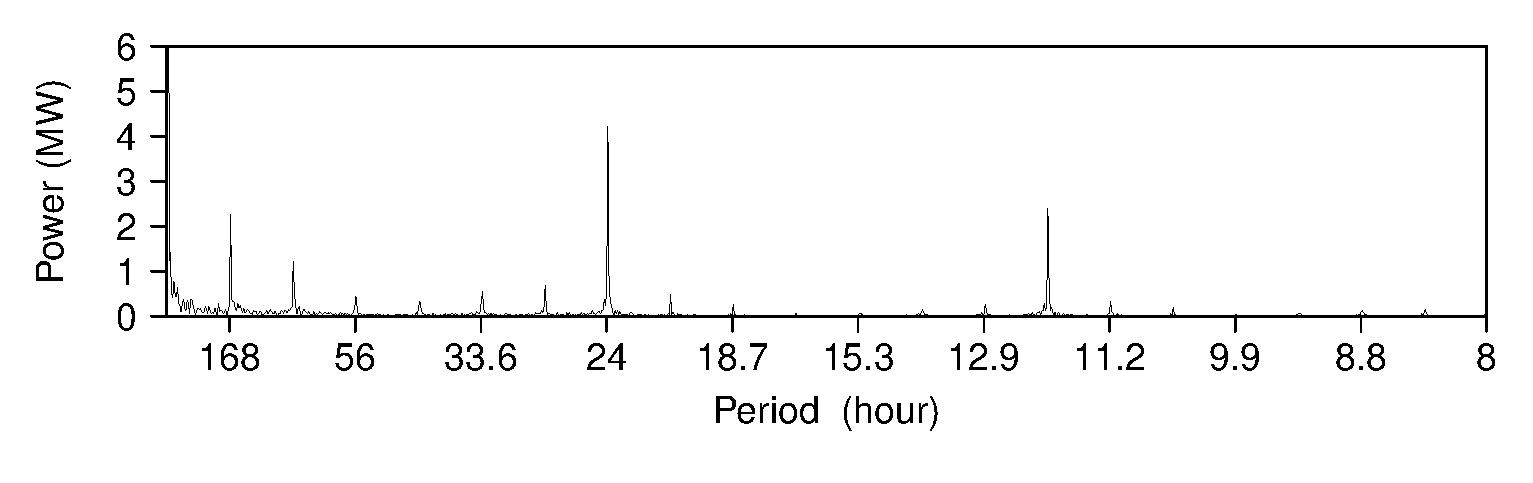
\includegraphics[width=10cm]{figs/plot_mufco_grid_nosc_fft.eps}
	%\end{center}
	%\vspace{-1.0cm}
	%\begin{columns}
	%\column{5cm}
		%\input{animations/smoothing.code}
	%\column{5cm}
		%\begin{center}
		%%{\bf Frequency filtering}\\
      %%[-0.3cm]
		%\begin{equation*}
		%\begin{array}{cc}
			%A^{nc}_{n} sin ( n \omega_{0} t + \phi^{nc}_{n} ) & \in P^{nc}(t) \\
			%A^{c}_{n}  sin ( n \omega_{0} t + \phi^{c}_{n})    & \in P^{c}(t)
		%\end{array}
		%\end{equation*}
		%\begin{equation*}
		%\begin{array}{cc}
			%\phi^{nc}_{n} \rightarrow - \phi^{c}_{n} & A^{c}_{n} \rightarrow A^{nc}_{n}
		%\end{array}
		%\end{equation*}
		%\end{center}
	%\end{columns}
%\end{frame}
%------------%

%\begin{frame}
	%\frametitle{Aggregated consumption}
	%\begin{center}	
	%%$P^{c}(t) = \displaystyle\sum\limits_{i=1}^{M} p^{c}_{i}(t)$\hspace{2cm}$P^{nc}(t) = \displaystyle\sum\limits_{i=1}^{M} p^{nc}_{i}(t)$
    %$P(t) = P^{c}(t) + P^{nc}(t) = \displaystyle\sum\limits_{i=1}^{M} p^{c}_{i}(t) + \displaystyle\sum\limits_{i=1}^{M} p^{nc}_{i}(t)$ 
	%\input{animations/grid_signals.code}
	%\end{center}
%\end{frame}
%%------------%
%\begin{frame}
	%\frametitle{Aggregated Consumption}
	%\begin{center}
	%\input{animations/mufco_demo.code}
	%\end{center}
%\end{frame}

%------------%
\begin{frame}
  \frametitle{Funciones de probabilidad}
  \centering
	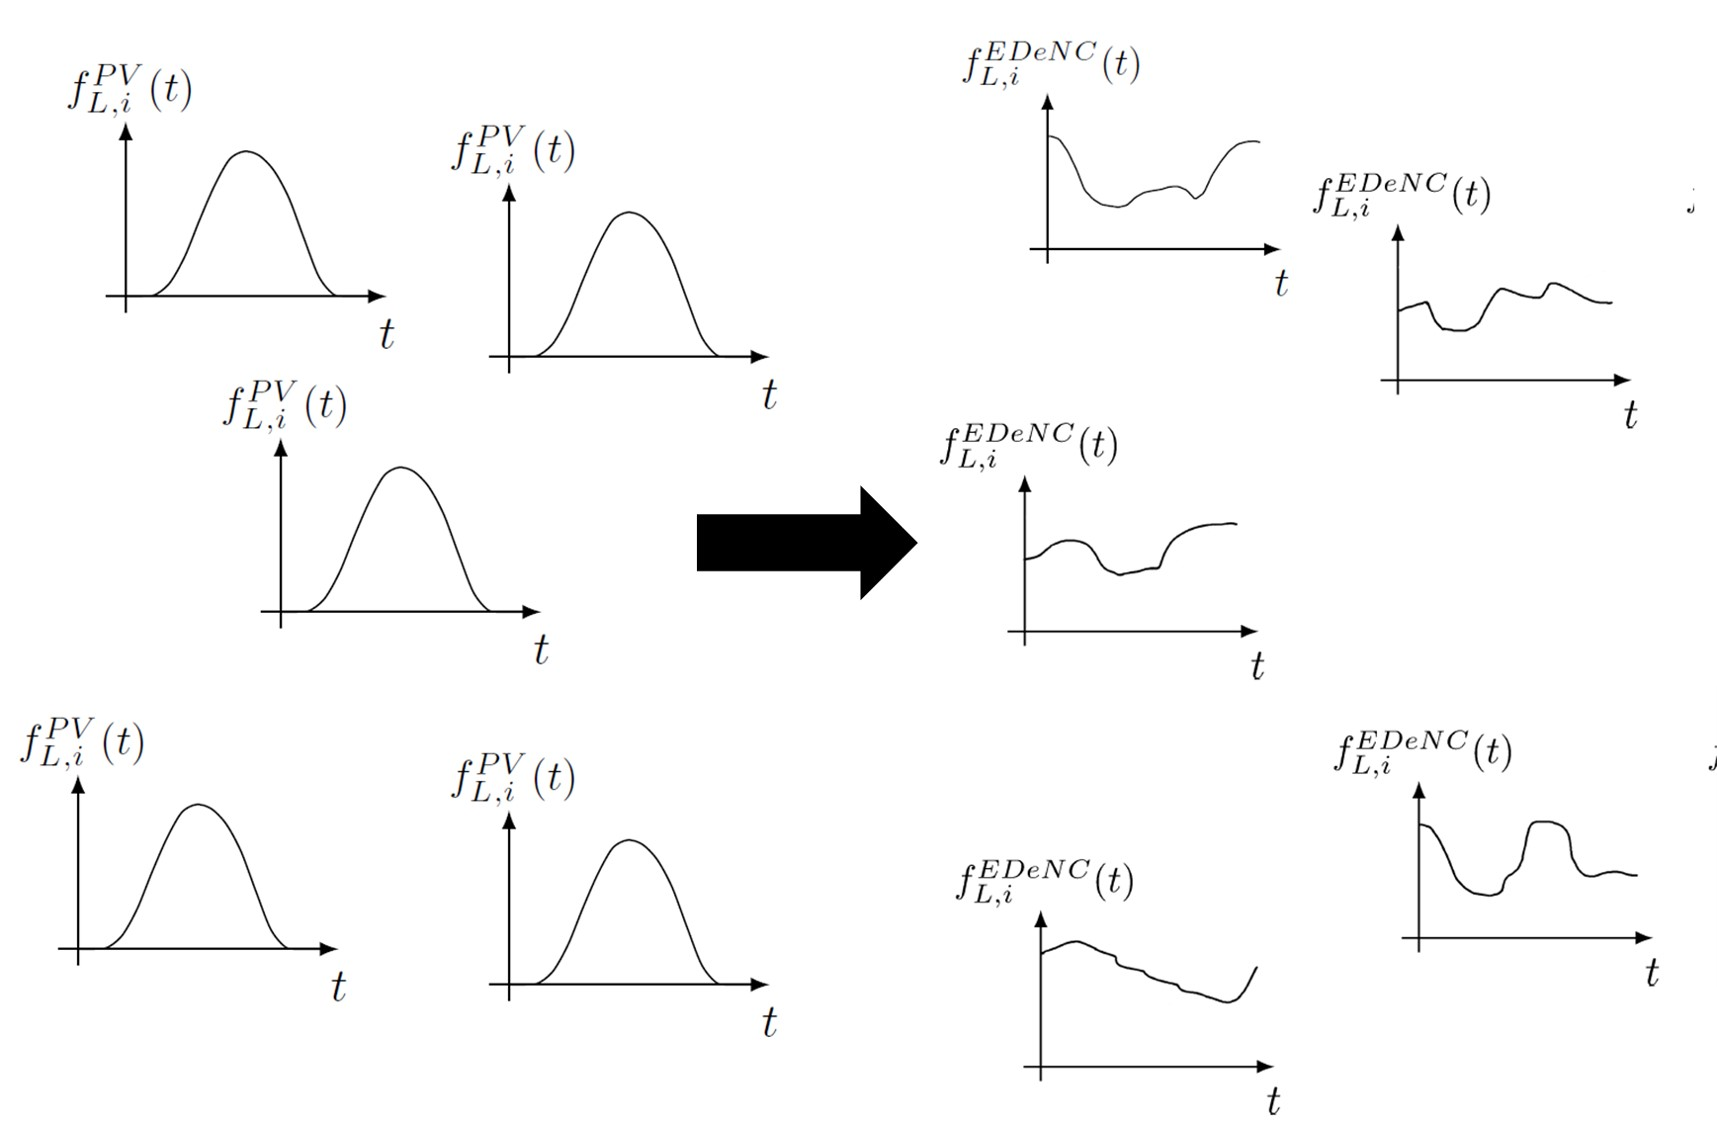
\includegraphics[width=10.4cm]{functs3}

  \begin{center}
    \begin{tabular}{p{6cm}p{6cm}}
      \textbf{Enfoque individual} &
      \textbf{Enfoque colaborativo}\\
    \end{tabular}
  \end{center}
\end{frame}

%------------%
%\begin{frame}
  %\frametitle{Virtual user}
  %\centering
	%\vspace{-1cm}	
	%\begin{center}	
	%Consumption is generated by ``virtual users''\\[0.5cm]
	%\begin{columns}
	%\column{5cm}
		%\begin{itemize}
		%\item{Deferrable load as ``energy packages''}
    %\visible<2->{\item{Generated in real time}}
    %\visible<3->{\item{Non-controllable distributed as aggregated consumption}}
    %%\item{Controllable distributed as Neural Grid}}
		%\end{itemize}
	%\column{8cm}
		%\begin{center}
		%\includegraphics<1>[width=4cm]{virtual_user_st1.eps}
		%\includegraphics<2>[width=7cm]{virtual_user_st2.eps}
    %\only<3>{\input{animations/virtual_user.code}}
		%\end{center}
	%\end{columns}
	%\end{center}		
%\end{frame}

%------------%
\begin{frame}
  \frametitle{Consumo agregado}
  \centering
	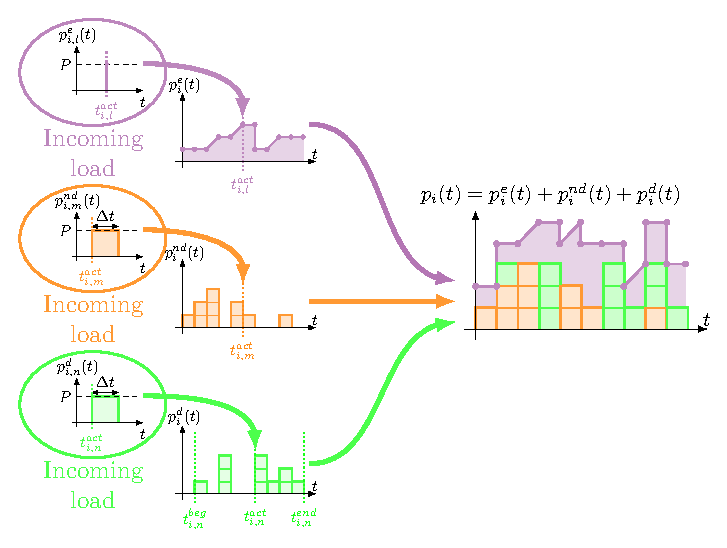
\includegraphics[width=9.4cm]{load_scheduling.eps}
\end{frame}

%------------%
%------------%

%\begin{frame}
	%\begin{center}
	%\frametitle{Aggregated Consumption}
	%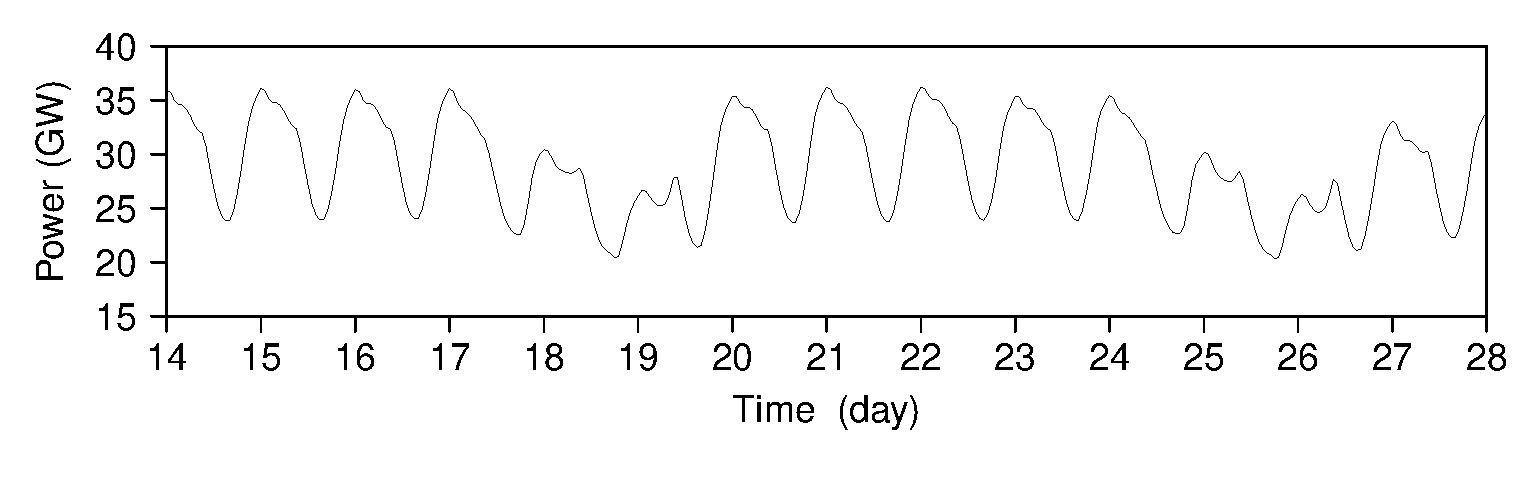
\includegraphics[width=11cm]{figs/plot_mufco_grid_nosc_week.eps}\\
	%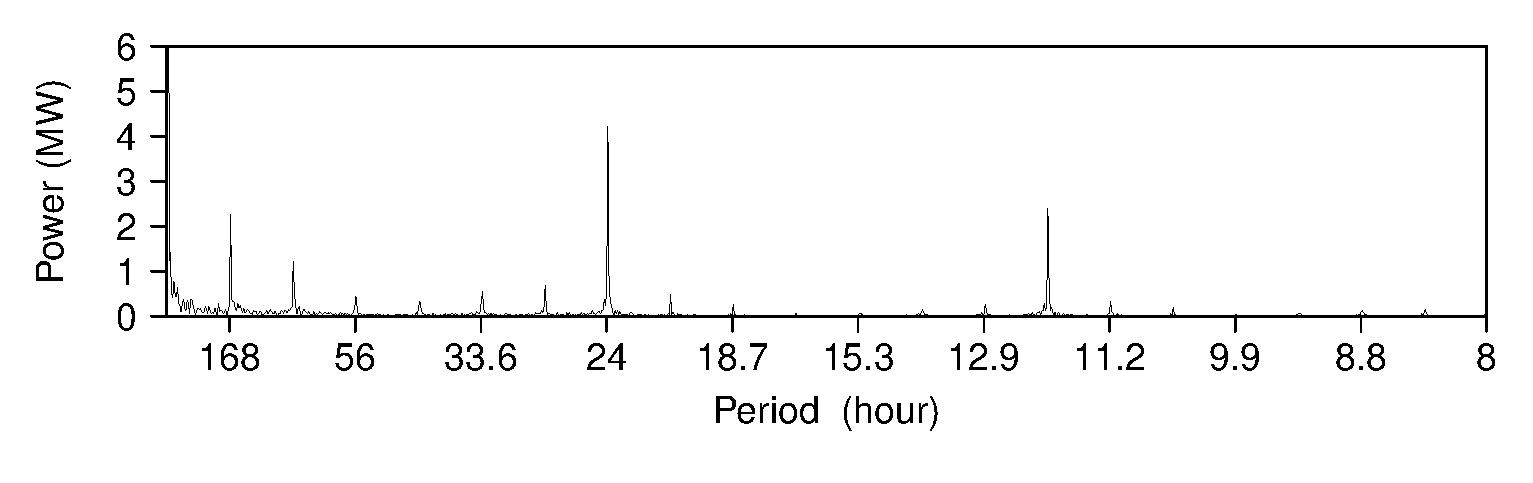
\includegraphics[width=11cm]{figs/plot_mufco_grid_nosc_fft.eps}
	%\end{center}
%\end{frame}

%------------%
\begin{frame}
  \frametitle{Evaluación}
  \begin{center}
    $f_{L,i}(t,\beta) = \beta \cdot f^{PV}_{L,i}(t) + (1 - \beta) \cdot f^{EDeNC}_{L,i}(t)$
  \end{center}
  \vspace{0.2cm} 
  \begin{columns}
    \column{5cm}
    \centering
    %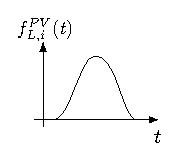
\includegraphics[width=4cm]{pvFunc.eps}
    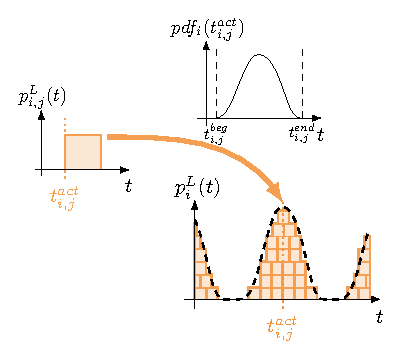
\includegraphics[width=5cm]{pv_profile.eps}
    \column{5cm}
    \centering
    %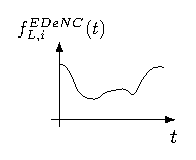
\includegraphics[width=4.25cm]{edencFunc.eps}
    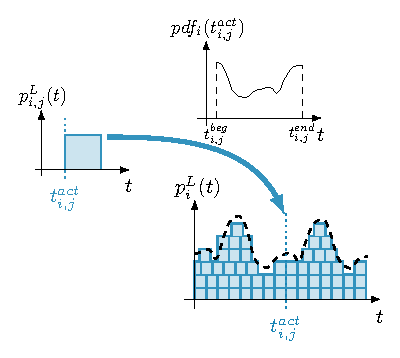
\includegraphics[width=5cm]{edenc_profile.eps}
  \end{columns}
  %\begin{itemize} 
    %\item 600 individuals (LEC/PED) 
      %\item Spanish peninsular aggregated consumption
      %\item Spanish peninsular PV generation and forecast 
  %\end{itemize} 
    %\visible<2->{
    %\begin{itemize}\item Analysis:
    %\begin{itemize}
      %\item Controllable load capacity: $L_{C}[\%] \in [0,100]$ 
      %\item PV penetration: $PV_p[\%] \in [0,100]$ 
      %\item Individual vs Collective: $\beta \in [0,1]$ 
      %%\item Battery capacity: $C_{bat}[d]$
    %\end{itemize}\end{itemize}}
\end{frame}

  \begin{frame}
  \frametitle{Evaluación}
  \begin{center}
    $f_{L,i}(t,\beta) = \beta \cdot f^{PV}_{L,i}(t) + (1 - \beta) \cdot f^{EDeNC}_{L,i}(t)$
  \end{center}
  
  \begin{columns}
    \column{5cm}
    \centering
    %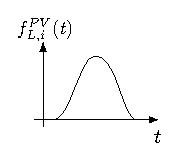
\includegraphics[width=4cm]{pvFunc.eps}
    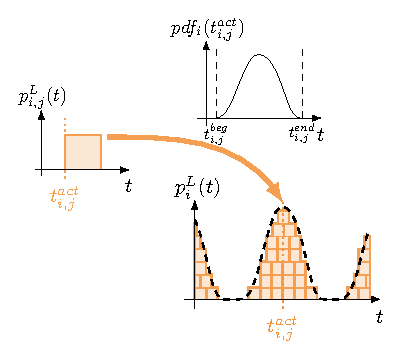
\includegraphics[width=5cm]{pv_profile.eps}
    \column{5cm}
    \centering
    %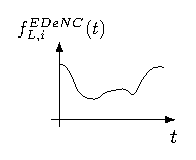
\includegraphics[width=4.25cm]{edencFunc.eps}
    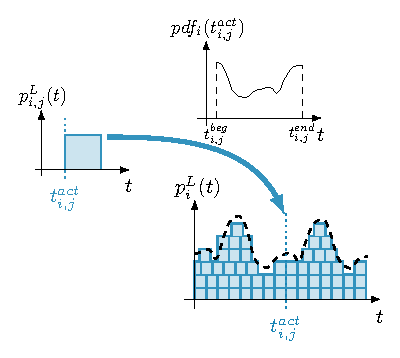
\includegraphics[width=5cm]{edenc_profile.eps}
  \end{columns}
  \begin{itemize} 
    %\item 600 individuals (LEC/PED) 
    \item Evaluación
  \end{itemize} 
    \begin{center}
      \begin{columns}
        \column{5cm}
        \centering
        Factor de cresta\\[0.2cm]
        {\large $C_f = \left. \frac{\lvert P \rvert_{peak}}{P_{rms}} \right|_{T}$}
        \column{5cm}
        \centering
        Autoconsumo\\[0.2cm]
        {\large $\xi_L = \frac{E_{PV,L} + E^{PV}_{B,L}}{E_{L}}$}
      \end{columns}
    \end{center}
\end{frame}
  
%------------%
\begin{frame}
  \frametitle{Evaluación}
  \begin{center}
    $f_{L,i}(t,\beta) = \beta \cdot f^{PV}_{L,i}(t) + (1 - \beta) \cdot f^{EDeNC}_{L,i}(t)$
  \end{center}

  \begin{columns}
    \column{5cm}
    \centering
    %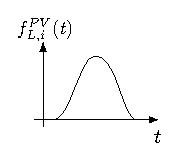
\includegraphics[width=4cm]{pvFunc.eps}
    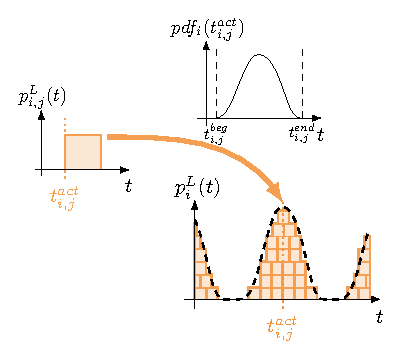
\includegraphics[width=5cm]{pv_profile.eps}
    \column{5cm}
    \centering
    %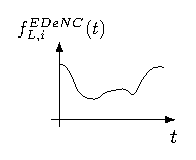
\includegraphics[width=4.25cm]{edencFunc.eps}
    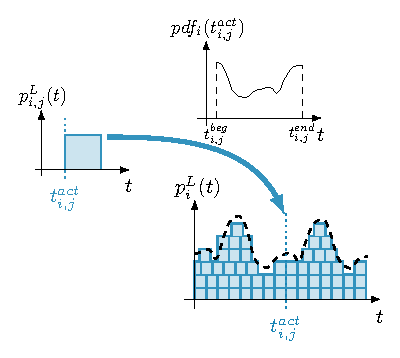
\includegraphics[width=5cm]{edenc_profile.eps}
  \end{columns}

  \begin{itemize} 
      %\item 600 individuals (LEC/PED) 
    \item Evaluación
      \begin{itemize}
        \item Cuanto más individual el enfoque ($\uparrow \beta$) $\rightarrow$ mayor $\xi_L$
        \item Cuanto más colectivo el enfoque ($\downarrow \beta$) $\rightarrow$ menor $C_f$
      \end{itemize}
  \end{itemize}

  \begin{center}
    Debe implementarse un compromiso entre el enfoque individual y el colectivo
  \end{center}

\end{frame}

%------------%
%\begin{frame}
  %\frametitle{Evaluation}
  %\vspace{0.2cm}
  %\begin{tabular}{m{5.5cm}m{5cm}}
    %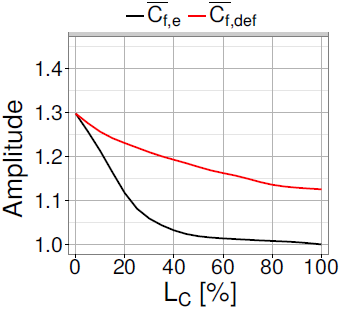
\includegraphics[width=3cm]{outro2} &
    %\begin{itemize}
      %\item $\nexists$ DSM $\rightarrow C_f > 1.0$
    %\end{itemize}\\
    %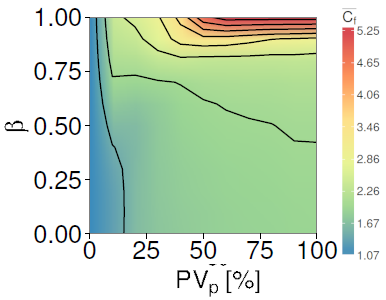
\includegraphics[width=3.3cm]{outro1} &
    %\begin{itemize}
      %\item $\uparrow$ indiv. $\rightarrow$ $\uparrow C_f$
      %\item $\uparrow$ PV $\rightarrow$ $\uparrow C_f$
    %\end{itemize}\\
    %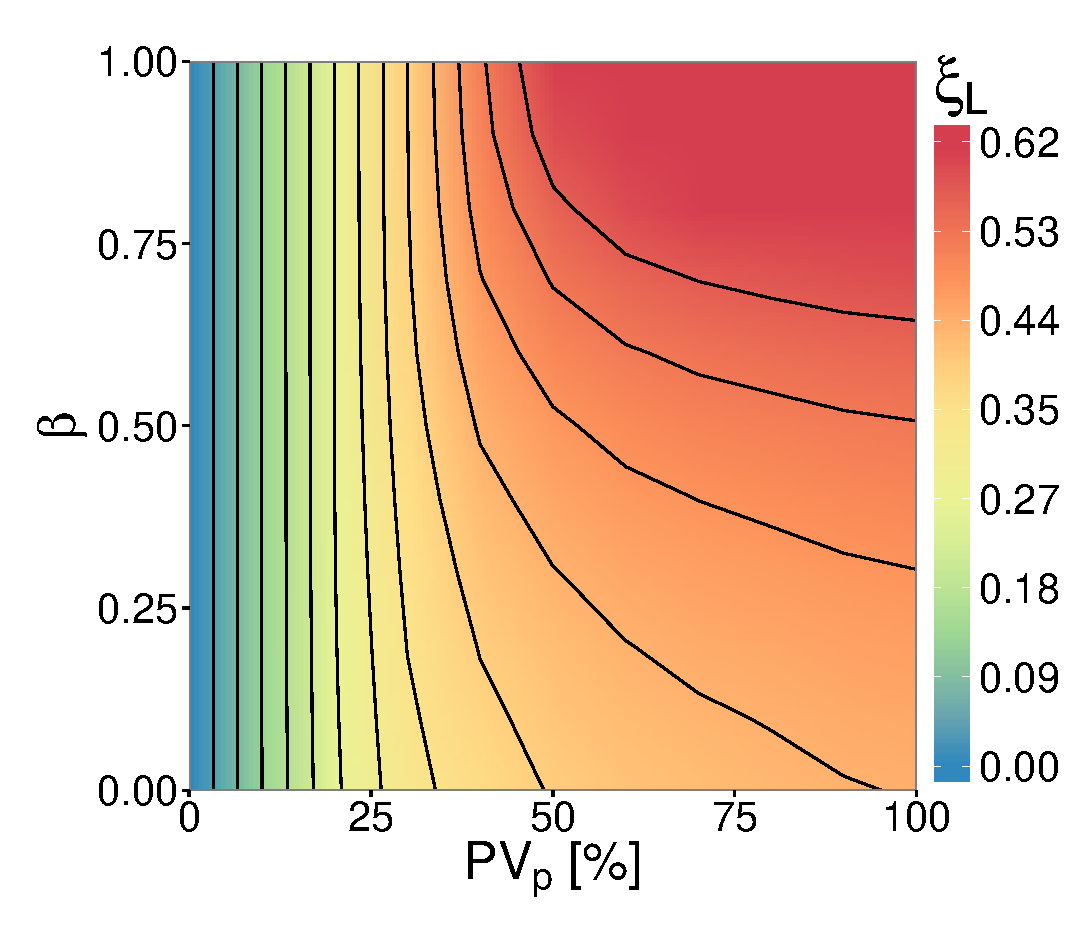
\includegraphics[width=3cm]{pvBEpsilon.eps}&
    %\begin{itemize}
      %\item $\uparrow$ PV $\rightarrow$ $\uparrow \xi_L$
      %\item $\uparrow$ indiv. $\rightarrow$ $\uparrow \xi_L$
    %\end{itemize}
  %\end{tabular}
 
%\end{frame}


%------------%
%\begin{frame}
  %\frametitle{Evaluation: $C_f$}
  %\begin{columns}
    %\column{7.5cm}
    %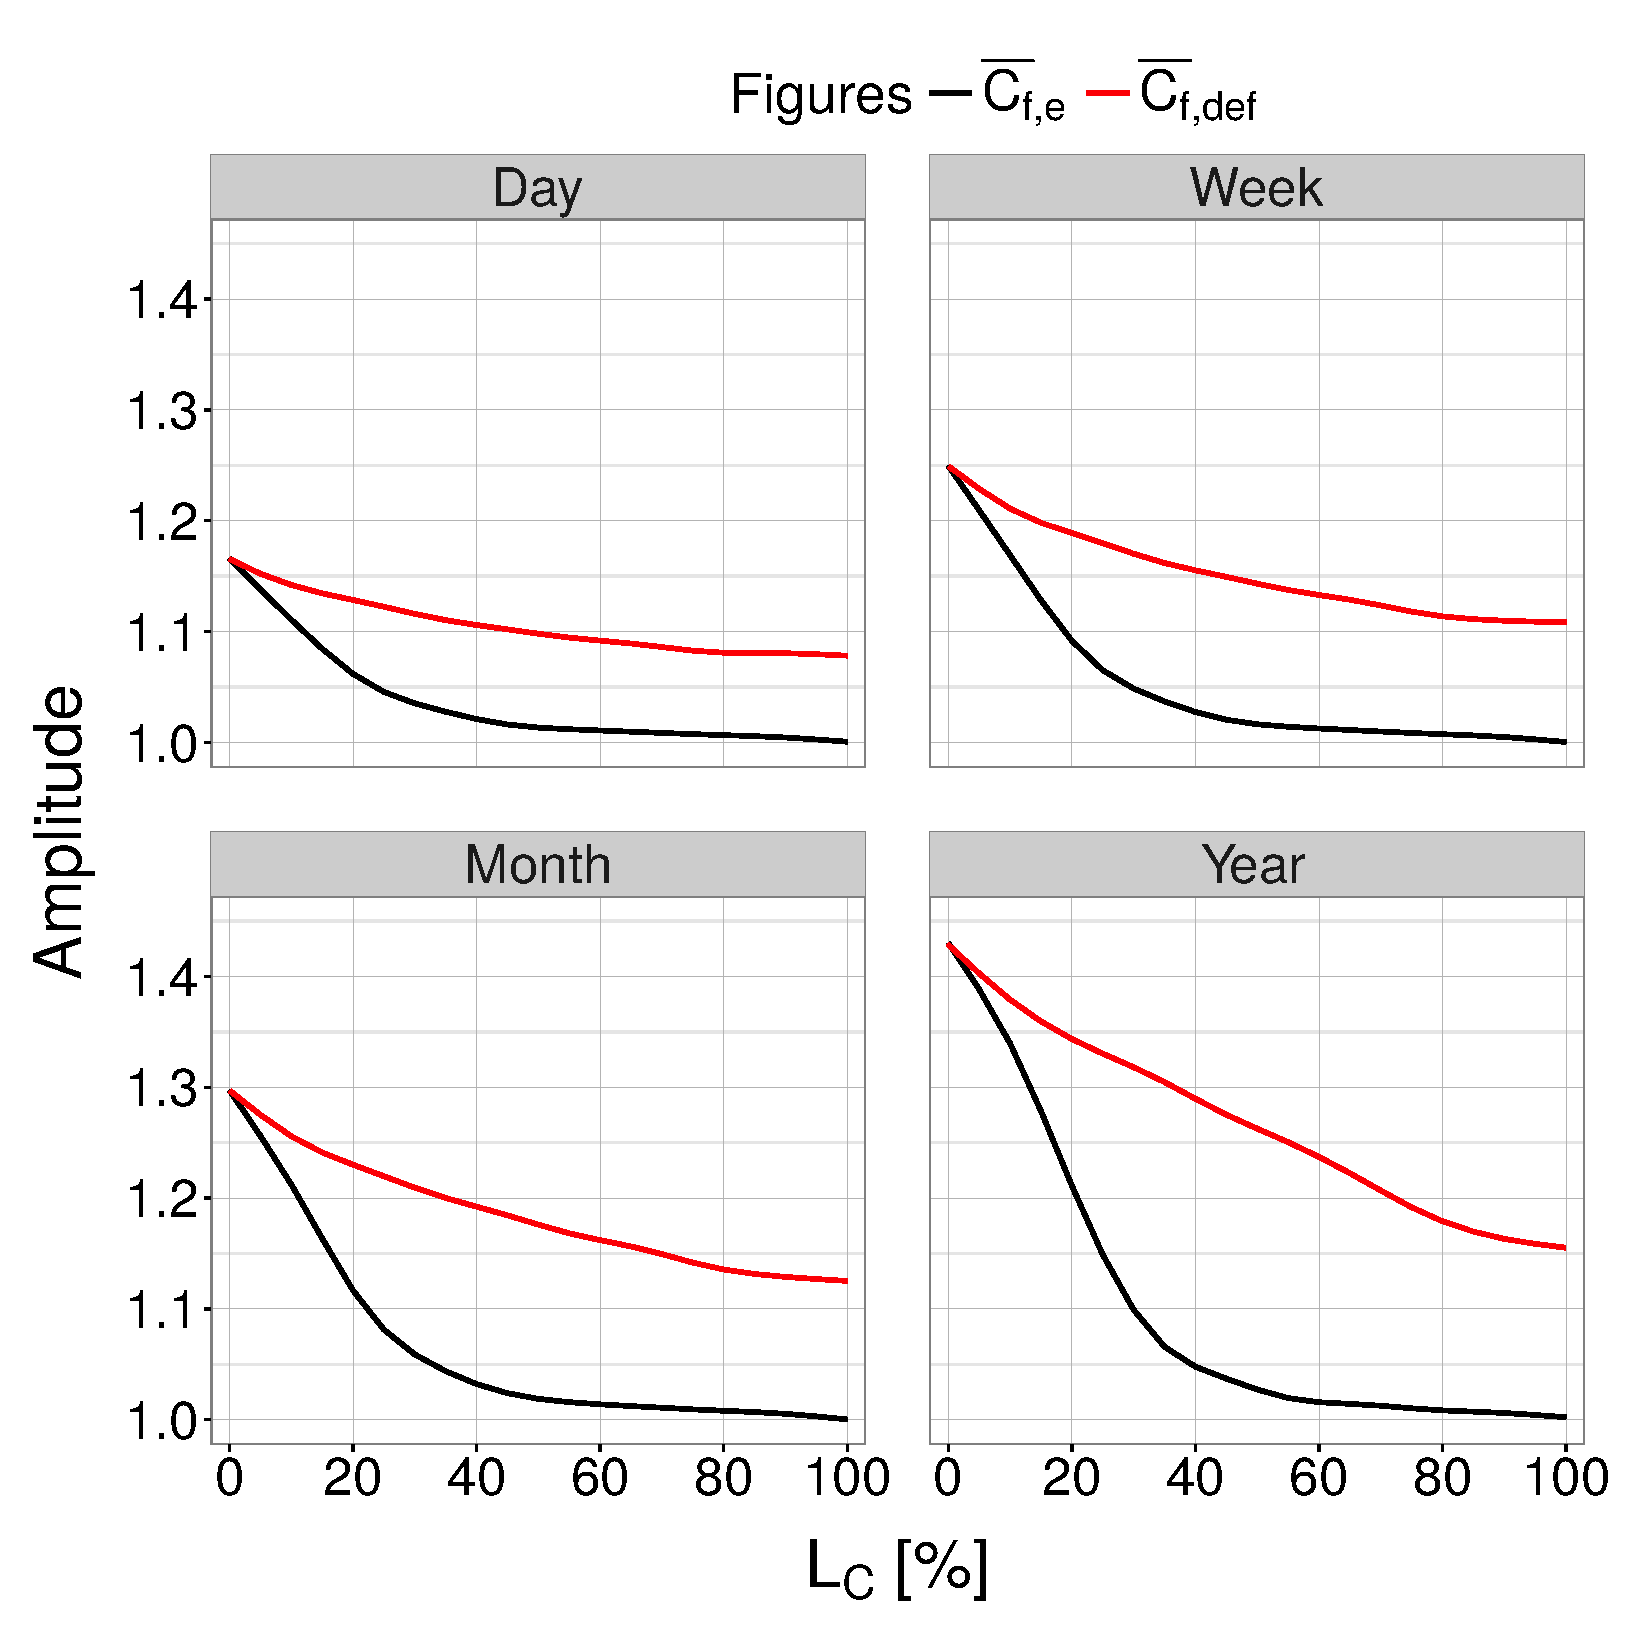
\includegraphics[width=7.25cm]{evalNCrt.eps} 
    %\column{2.5cm}
    %\textcolor{red}{---} No-DSM\\
    %\textcolor{black}{---} DSM
  %\end{columns}
%\end{frame}

%%------------%
%\begin{frame}
  %\frametitle{Evaluation: $C_f$}
  %\centering
  %\begin{columns}
    %\column{8cm}
	    %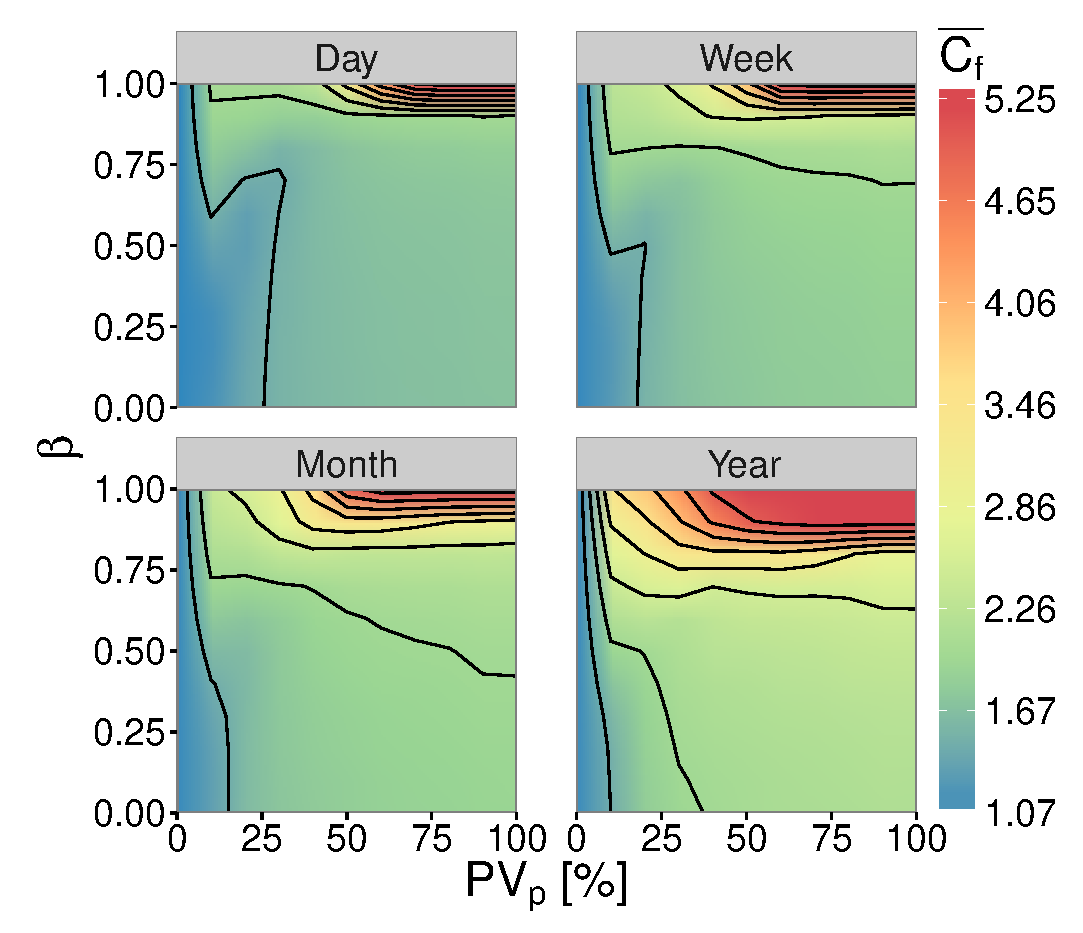
\includegraphics[width=8cm]{pvB.eps}
    %\column{2.5cm}
      %{$L_C=100\,\%$}\\
      %$\uparrow$ indiv. $\rightarrow$ $\uparrow C_f$\\
      %$\uparrow$ PV $\rightarrow$ $\uparrow C_f$
  %\end{columns}
%\end{frame}

%%------------%
%\begin{frame}
  %\frametitle{Evaluation: $\xi_L$}
  %\centering
  %\begin{columns}
    %\column{8cm}
	    %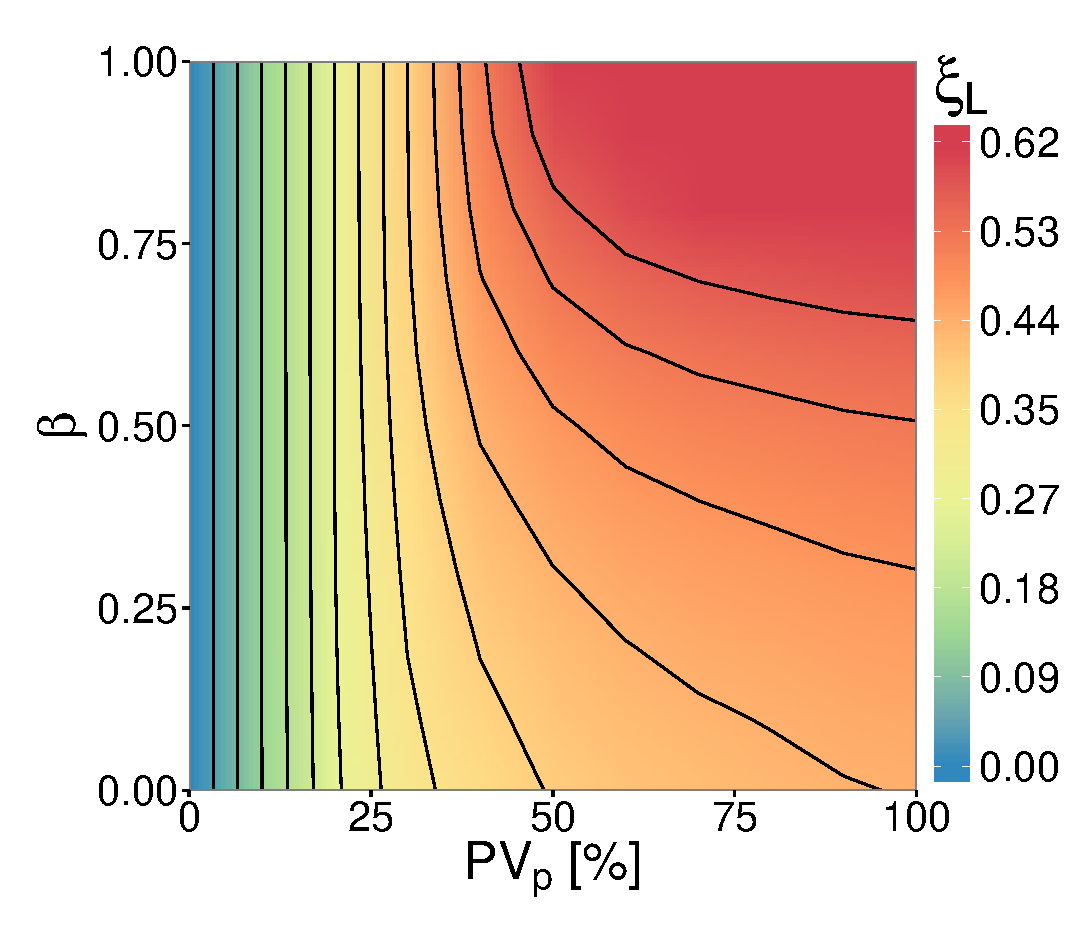
\includegraphics[width=8cm]{pvBEpsilon.eps}
    %\column{2.5cm}
      %{$L_C=100\,\%$}\\
      %$\uparrow$ PV $\rightarrow$ $\uparrow \xi_L$\\
      %$\uparrow$ indiv. $\rightarrow$ $\uparrow \xi_L$
  %\end{columns}
%\end{frame}

%%------------%
%\begin{frame}
  %\frametitle{Evaluation: $C_f$}
  %\centering
  %\begin{columns}
    %\column{8cm}
      %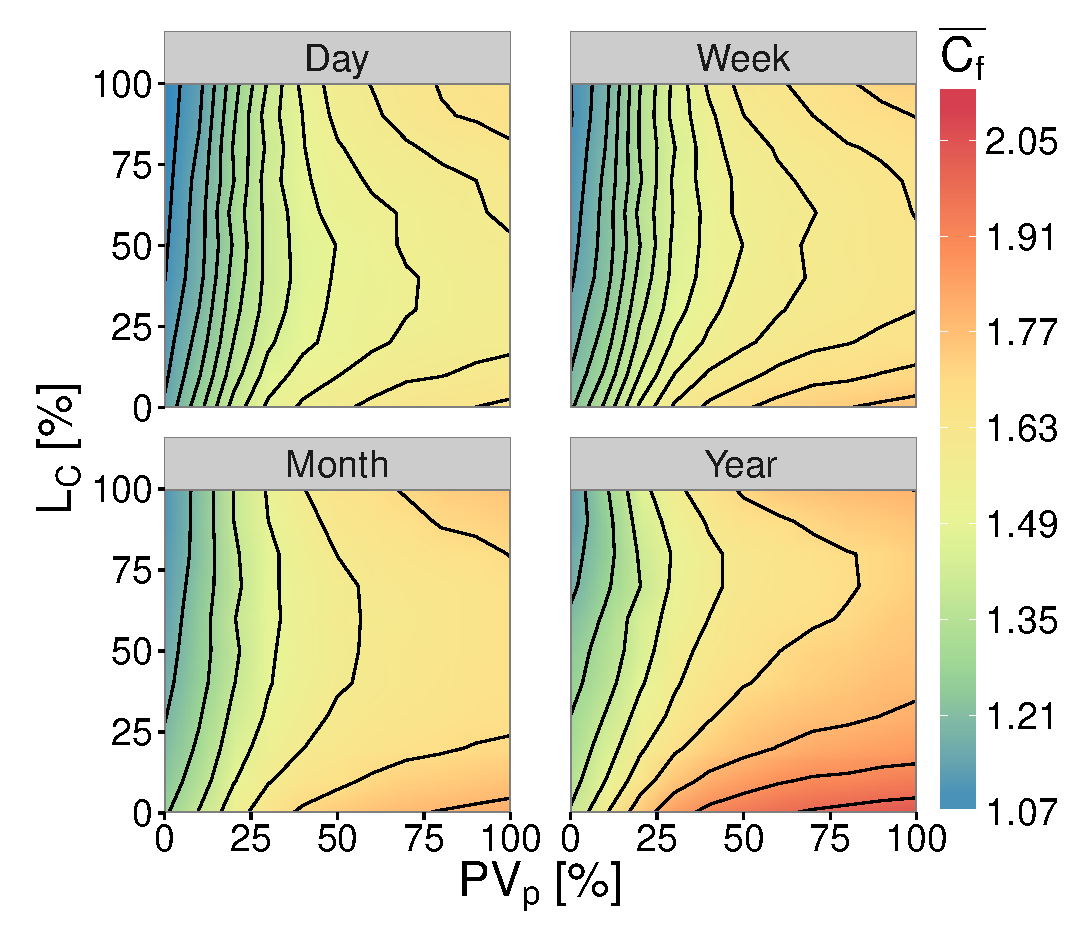
\includegraphics[width=8cm]{pvCtr.eps}
    %\column{2.5cm}
      %$\beta=0$\\
      %$\uparrow$ $L_c$ $\rightarrow$ $\downarrow C_f$\\
      %$\uparrow$ $PV$ $\rightarrow$ $\uparrow C_f$
  %\end{columns}
%\end{frame}

%------------%
%\begin{frame}
  %\frametitle{Evaluation: $\xi_L$}
  %\centering
  %\begin{columns}
    %\column{8cm}
      %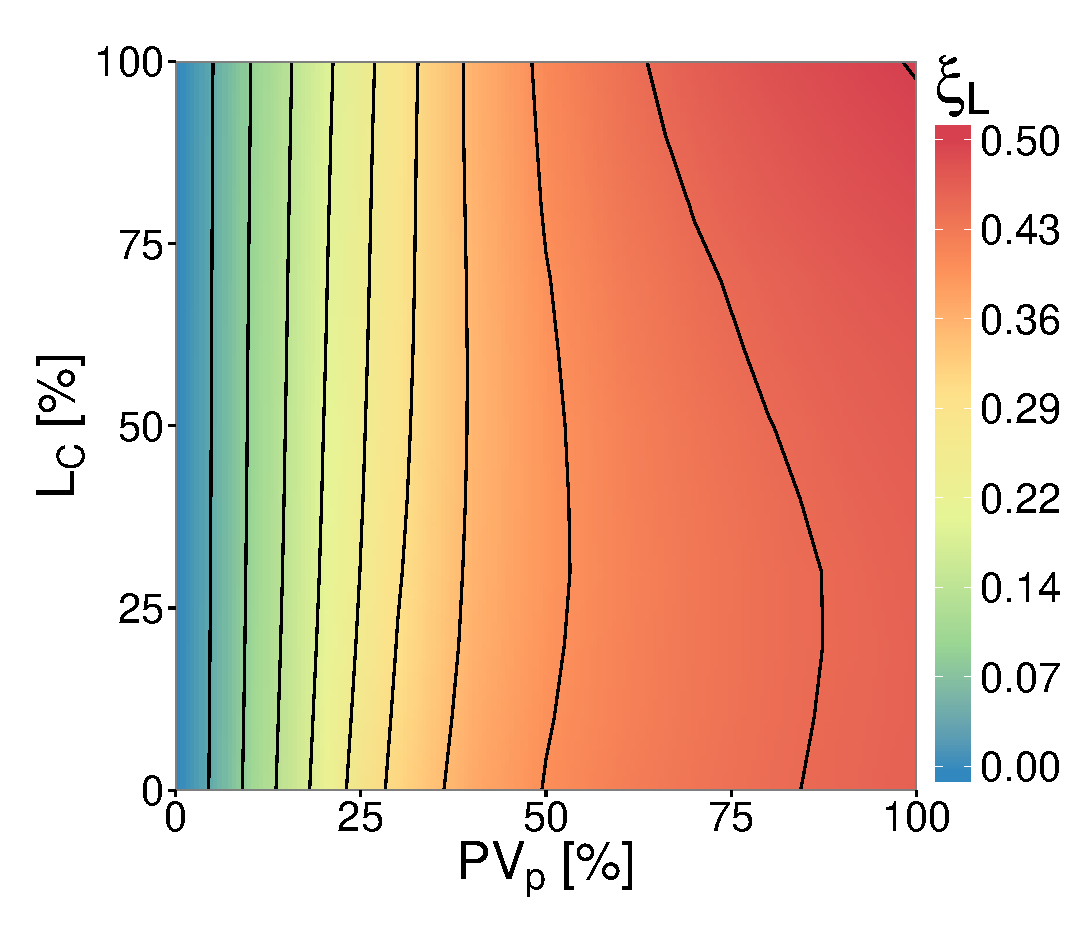
\includegraphics[width=8cm]{pvCtrEpsilon.eps}
    %\column{2.5cm}
      %\centering
      %$\beta=0$\\
      %$\uparrow$ $PV$ $\rightarrow$ $\uparrow \xi_L$\\
      %$\uparrow$ $L_c$ $\rightarrow$ $\approx \xi_L$
  %\end{columns}
%\end{frame}

%\begin{frame}
	%\frametitle{Summary }
	%{\bf Social Insects features:}
	%\begin{itemize}
	%\item{{\bf Adaptability}: }$P^{c}(t)$ adapts to $P^{nc}(t)$
	%\item{{\bf Self-organization}: }scheduling without central agent	
	%\item{{\bf Low information exchange}:} only aggregated consumption
	%\item{{\bf Local conditions}:} local PV generation and consumption
	%\end{itemize}
	%\visible<2->{
	%{\bf Effects on the aggregated consumption:}
	%\begin{itemize}
    %\item{Aggregated consumption is smoothed}
    %\item{Adapts to the PV generation}
    %\item Variability depends on the swarm objective 
    %\item Self-Consumption increases
	%\end{itemize}}
%\end{frame}



%------------%

\begin{frame}
	\frametitle{Resumen}
  \begin{center}
    \textbf{QUEDA MUCHO POR HACER}, \\
    tanto en investigación como en implementación\\
    \vspace{0.2cm}
    Mientras tanto\\
    \vspace{0.3cm}
    \textbf{Imagina un árbol resplandeciendo como si una luciérnaga \\
    reposara en cada hoja, todas destellando periódicamente, \\
    con oscuridad entre los destellos. Extiende esto a un \\
    grupo de árboles que pulsan en perfecta unisonancia, \\
    un ritmo sobrecogedor de luz viva.\\}
    \tiny{\textit{Adaptado de H. M. Smith, Science, 1935}}
  \end{center}

    %\begin{center}
      %\begin{tabular}{cc}
      %\iftoggle{video}
      %{
        %%\hspace{-1cm}
        %\animategraphics[autoplay,loop,width=5cm]{10}{mov/fireflies/}{1}{1148} &
        %\animategraphics[loop,width=5cm]{10}{mov/cities/}{1}{399}  \\
        %%Red Neuronal Biológica & Red Neuronal Artificial \\
      %}
      %{
        %%\hspace{-1cm}
        %\includegraphics[width=6cm]{mov/fireflies/400.eps} &
        %\includegraphics[width=6cm]{mov/cities/1.eps} \\
        %%Red Neuronal Biológica & Red Neuronal Artificial \\
      %}
      %\end{tabular}
    %\end{center}
    
    \begin{center}
      \begin{tabular}{cc}
        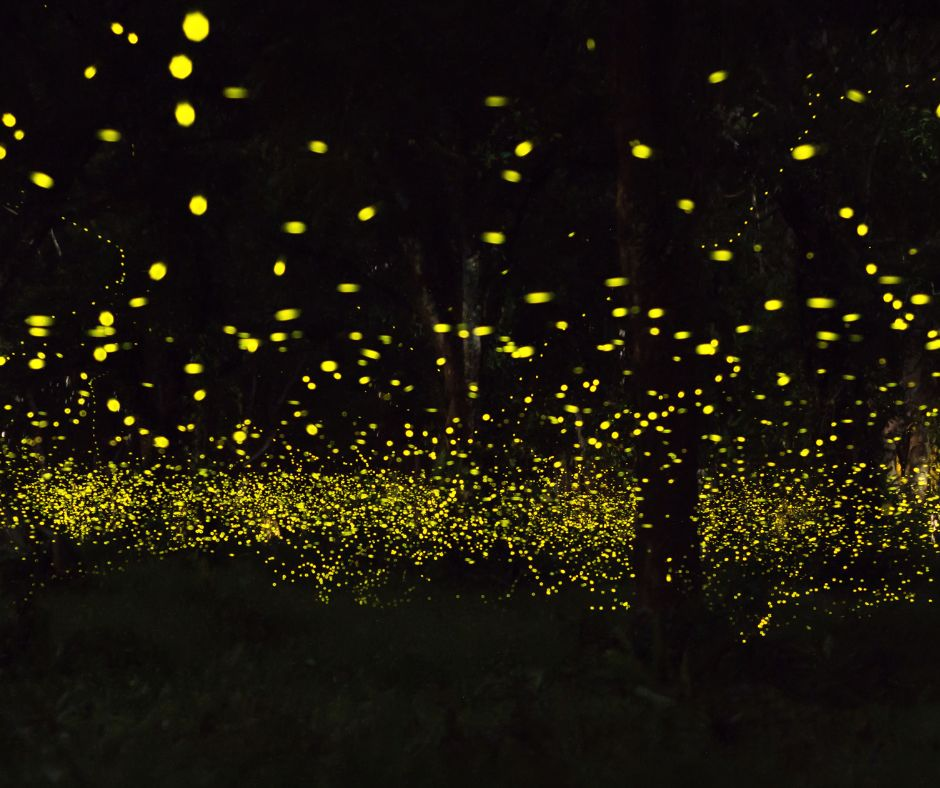
\includegraphics[width=3.5cm]{figs/firefliesV2.jpg} &
        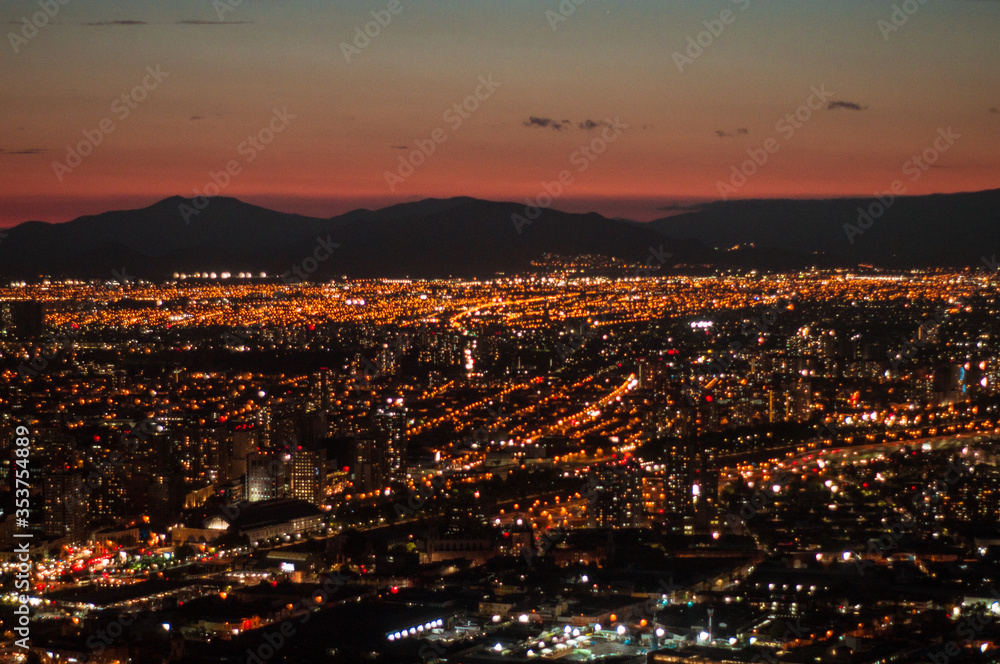
\includegraphics[width=4.5cm]{figs/ciudadNoche.jpg} \\
      \end{tabular}
    \end{center}
\end{frame}

\begin{frame}[plain]
  \titlepage
\end{frame}
\end{document}

%------------%
%\begin{frame}
	%\frametitle{Actual research}
  %\begin{itemize}
    %\item WOS Search (10/2025):
  %\footnotesize{
	%%\begin{itemize}
    %\item Swarm + Energy: 26652 matchs. (15341 >2020)
    %%\item Swarm intelligence + energy: 2334 matchs (all >2020)
    %%\item Swarm intelligence + energy management: 893 (all >2020)
    %%\item Swarm intelligence + demand management: 395 (all >2020)
    %%\item Swarm intelligence + energy demand management: 233 (all >2020)
    %%\item Swarm intelligence + demand side management: 57 (all >2020)
    %%\item Swarm intelligence + local energy: 426 (all >2020)
    %%\item Swarm intelligence + local energy comunities: 11 (all >2020)
    %\item Swarm + energy management: 8876 (5910) >2020)
    %\item Swarm + demand management: 4688 (2783 >2020)
    %\item Swarm + energy demand management: 2798 (1868 >2020)
    %\item Swarm + demand side management: 955 (581 >2020)
    %\item Swarm + local energy: 3351 (2145 >2020)
    %\item Swarm + local energy comunities: 78 (57 >2020)
	%%\end{itemize}
%}
	%\end{itemize}
  %\begin{center}
    %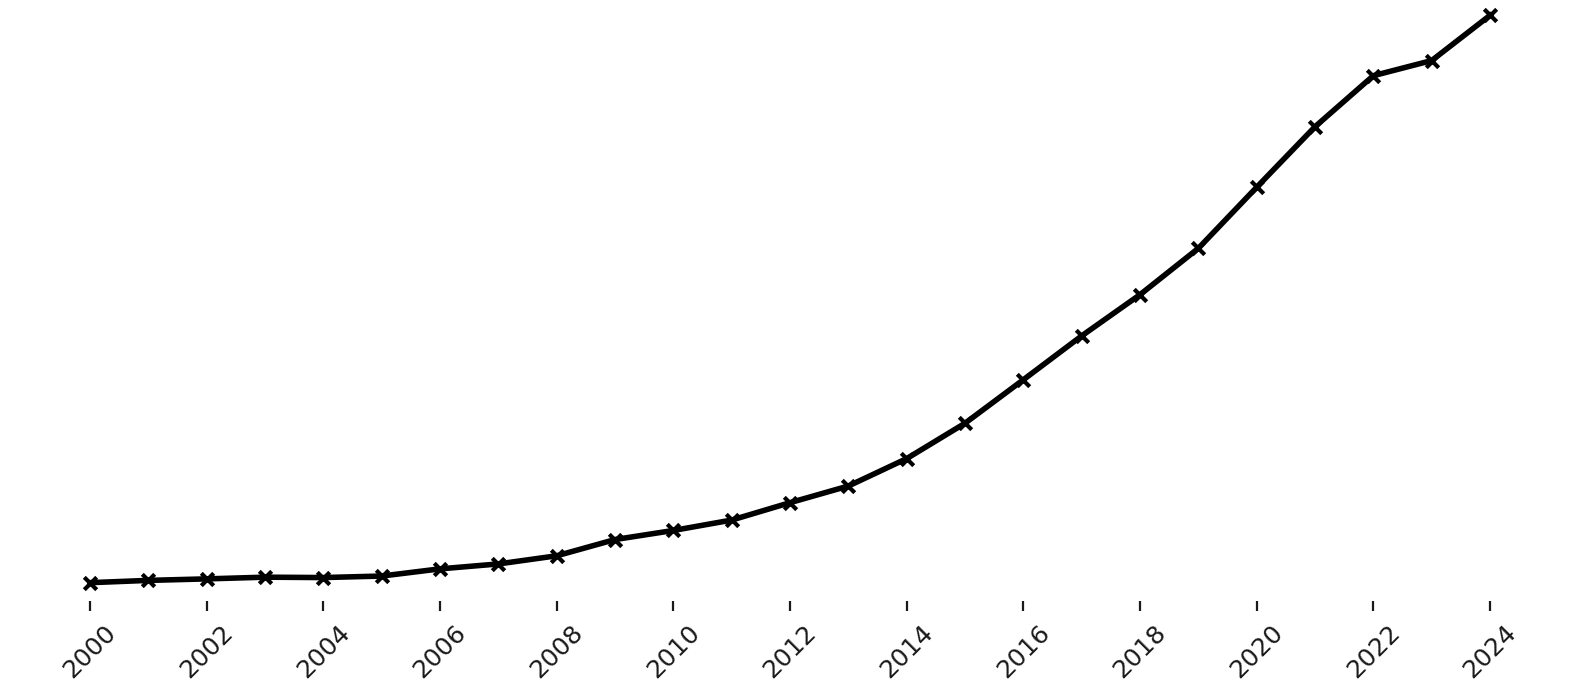
\includegraphics[width=8cm]{figs/publicationsChart}
  %\end{center}
%\end{frame}
